\begin{bt}%[2D4N1-4]
% nguon: Archive/2024/0. [LVH] BG - 12 New - 4in1-20240625T224301Z-001/0. [LVH] BG - 12 New - 4in1/2. [LVH] TEX SGK 12 NEW-20240418T074833Z-001/2. [LVH] TEX SGK 12 NEW/[LVH] SGK-12-KNTT/data/C4/12-c4-Bai11-nguyenham.tex #1156

	Trong mỗi trường hợp sau, hàm số $F(x)$ có là một nguyên hàm của hàm số $f(x)$ trên khoảng tương ứng không? Vì sao?
	\begin{enumerate}[a)]
		\item $F(x) = x\ln x$ và $f(x) = 1 + \ln x$ trên khoảng $(0;+\infty)$;
		\item $F(x) = e^{\sin x}$ và $f(x) = e^{\cos x}$ trên $\mathbb{R}$.
	\end{enumerate}
	\loigiai{
	\begin{enumerate}[a)]
		\item Vì $F'(x)=\ln x+x\cdot \left (\ln x \right )'=1+\ln x=f(x)$ nên $F(x)$ là một nguyên hàm của hàm số $f(x)$.
		\item Vì $F'(x)=(\sin x)'\mathrm{e}^{\sin x}=\cos x\mathrm{e}^{\sin x}\ne f(x)$ nên $F(x)$ không phải là một nguyên hàm của $f(x)$.
	\end{enumerate}
	}
\end{bt}

\begin{bt}%[2D4N1-2]
% nguon: Archive/2024/0. [LVH] BG - 12 New - 4in1-20240625T224301Z-001/0. [LVH] BG - 12 New - 4in1/2. [LVH] TEX SGK 12 NEW-20240418T074833Z-001/2. [LVH] TEX SGK 12 NEW/[LVH] SGK-12-KNTT/data/C4/12-c4-Bai11-nguyenham.tex #1157
 
	Tìm nguyên hàm của các hàm số sau:
	\begin{enumerate}[a)]
		\item $f(x) = 3x^2 + 2x - 1$;
		\item $f(x) = x^3-x$;
		\item $f(x) = (2x+1)^2$;
		\item $f(x) = \left (2x-\dfrac{1}{x}\right )^2$.
	\end{enumerate}
\loigiai{
	\begin{enumerate}[a)]
		\item $\displaystyle \int \left (3x^2 + 2x - 1\right ) \mathrm{\,d}x = x^3 + x^2 - x + C.$
		
		\item $\displaystyle \int \left (x^3 - x\right ) \mathrm{\,d}x = \frac{x^4}{4} - \frac{x^2}{2} + C.$
		
		\item $\displaystyle \int \left (2x+1\right )^2 \mathrm{\,d}x =\int (4x^2+4x+1) \mathrm{\,d}x= \frac{4x^3}{3} + 2x^2 + x + C.$
		
		\item $\displaystyle \int \left (2x-\frac{1}{x}\right )^2\mathrm{\,d}x =\int \left (4x^2-4+\frac{1}{x^2}\right )\mathrm{\,d}x = \frac{4x^3}{3} - 4x - \frac{1}{x} + C.$
	\end{enumerate}
}
\end{bt}

\begin{bt}%[2D4H1-2]
% nguon: Archive/2024/0. [LVH] BG - 12 New - 4in1-20240625T224301Z-001/0. [LVH] BG - 12 New - 4in1/2. [LVH] TEX SGK 12 NEW-20240418T074833Z-001/2. [LVH] TEX SGK 12 NEW/[LVH] SGK-12-KNTT/data/C4/12-c4-Bai11-nguyenham.tex #1158
 
	Tìm:
	\begin{enumerate}[a)]
		\item $\displaystyle\int\left (3\sqrt{x}+\dfrac{1}{\sqrt[3]{x}}\right )\mathrm{\,d}x$;
		\item $\displaystyle\int\sqrt{x}(7x^2-3)\mathrm{\,d}x$ ($x>0$);
		\item $\displaystyle\int \dfrac{(2x+1)^2}{x^2}\mathrm{\,d}x$;
		\item $\displaystyle\int \left (2^x + \dfrac{3}{x^2}\right )\mathrm{\,d}x$.
	\end{enumerate}
\loigiai{
\begin{enumerate}[a)]
	\item $\displaystyle\int\left (3\sqrt{x}+\dfrac{1}{\sqrt[3]{x}}\right )\mathrm{\,d}x = \int \left( 3x^{1/2} + x^{-1/3}\right)  \mathrm{\,d}x = \frac{6}{3}x^{3/2} + \dfrac{3}{2}x^{2/3} + C = 2x^{3/2} + \dfrac{3}{2}x^{2/3} + C.$
	
	\item $\displaystyle\int\sqrt{x}(7x^2-3)\mathrm{\,d}x = \int 7x^{5/2} - 3x^{1/2} \mathrm{\,d}x = \frac{14}{7}x^{7/2} - 2x^{3/2} + C = 2x^{7/2} - 2x^{3/2} + C.$
	
	\item $\displaystyle\int \dfrac{(2x+1)^2}{x^2}\mathrm{\,d}x = \int \frac{4x^2 + 4x + 1}{x^2} \mathrm{\,d}x = \int \left (4 + \frac{4}{x} + \frac{1}{x^2}\right ) \mathrm{\,d}x = 4x - 4\ln|x| - \frac{1}{x} + C.$
	
	\item $\displaystyle\int \left (2^x + \dfrac{3}{x^2}\right )\mathrm{\,d}x = \int 2^x \mathrm{\,d}x + \int \frac{3}{x^2} \mathrm{\,d}x = \frac{2^x}{\ln 2} - \frac{3}{x} + C.$
\end{enumerate}

}
\end{bt}

\begin{bt}%[2D4H1-3]
% nguon: Archive/2024/0. [LVH] BG - 12 New - 4in1-20240625T224301Z-001/0. [LVH] BG - 12 New - 4in1/2. [LVH] TEX SGK 12 NEW-20240418T074833Z-001/2. [LVH] TEX SGK 12 NEW/[LVH] SGK-12-KNTT/data/C4/12-c4-Bai11-nguyenham.tex #1159

	Tìm:
	\begin{enumerate}[a)]
		\item $\displaystyle\int (2\cos x - \dfrac{3}{\sin^2 x})\mathrm{\,d}x$;
		\item $\displaystyle\int 4\sin^2\dfrac{x}{2}\mathrm{\,d}x$;
		\item $\displaystyle\int (\sin \dfrac{x}{2} - \cos \dfrac{x}{2})^2\mathrm{\,d}x$;
		\item $\displaystyle\int (x+\tan^2 x)\mathrm{\,d}x$.
	\end{enumerate}
	\loigiai{
	\begin{enumerate}[a)]
		\item $\displaystyle\int \left (2\cos x - \dfrac{3}{\sin^2 x}\right )\mathrm{\,d}x = 2\sin x + 3\cot x + C$.
		
		\item $\displaystyle\int 4\sin^2\dfrac{x}{2}\mathrm{\,d}x = 2\int (1 - \cos x) \mathrm{\,d}x = 2(x - \sin x) + C$.
		
		\item $\displaystyle\int \left (\sin \dfrac{x}{2} - \cos \dfrac{x}{2}\right )^2\mathrm{\,d}x = \int \left (1-\sin x\right )\mathrm{\,d}x= x+\cos x + C.$
		
		\item $\displaystyle\int (x+\tan^2 x)\mathrm{\,d}x = \int (x-1)\mathrm{\,d}x + \int \left (1+\tan^2 x\right )\mathrm{\,d}x = \frac{x^2}{2} - x + \tan x + C$.
	\end{enumerate}
	
	}
\end{bt}

\begin{bt}%[2D4H1-2]
% nguon: Archive/2024/0. [LVH] BG - 12 New - 4in1-20240625T224301Z-001/0. [LVH] BG - 12 New - 4in1/2. [LVH] TEX SGK 12 NEW-20240418T074833Z-001/2. [LVH] TEX SGK 12 NEW/[LVH] SGK-12-KNTT/data/C4/12-c4-Bai11-nguyenham.tex #1160
 
	Cho hàm số $y = f(x)$ xác định trên khoảng $(0; +\infty)$. Biết rằng, $f'(x) = 2x + \dfrac{1}{x^2}$ với mọi $x \in (0; +\infty)$ và $f(1) = 1$. Tính giá trị $f(4)$.
	\loigiai{
	Ta có $\displaystyle f(x)=\int f'(x)\mathrm{\,d}x=\int \left (2x+\frac{1}{x^2}\right )\mathrm{\,d}x= x^2-\dfrac{1}{x}+C $.\\
	Mà $f(1)=1$ nên $C=1$. Vậy $f(4)=\dfrac{67}{4}$.
	}
\end{bt}

\begin{bt}%[2D4H1-2]
% nguon: Archive/2024/0. [LVH] BG - 12 New - 4in1-20240625T224301Z-001/0. [LVH] BG - 12 New - 4in1/2. [LVH] TEX SGK 12 NEW-20240418T074833Z-001/2. [LVH] TEX SGK 12 NEW/[LVH] SGK-12-KNTT/data/C4/12-c4-Bai11-nguyenham.tex #1161
 
	Cho hàm số $y = f(x)$ có đồ thị là $(C)$. Xét điểm $M(x; f(x))$ thay đổi trên $(C)$. Biết rằng, hệ số góc của tiếp tuyến của đồ thị $(C)$ tại $M$ là $k_M = (x - 1)^2$ và điểm $M$ trùng với gốc toạ độ khi nó nằm trên trục tung. Tìm biểu thức $f(x)$.
	\loigiai{
	Theo đề bài ta có $f'(x)=(x-1)^2$, suy ra 
	\[f(x)= \int (x-1)^2\mathrm{\,d}x=\int (x-1)^2\mathrm{\,d}(x-1)=\dfrac{(x-1)^3}{3}+C\]
	Vì $M$ trùng với gốc tọa độ khi nó nằm trên trục tung nên 
	$ f(0)=0\Leftrightarrow C=\dfrac{1}{3}.$\\
	Vậy $f(x)=\dfrac{(x-1)^3}{3}+\dfrac{1}{3}$.
	}
\end{bt}

\begin{bt}%[2D4V1-6]
% nguon: Archive/2024/0. [LVH] BG - 12 New - 4in1-20240625T224301Z-001/0. [LVH] BG - 12 New - 4in1/2. [LVH] TEX SGK 12 NEW-20240418T074833Z-001/2. [LVH] TEX SGK 12 NEW/[LVH] SGK-12-KNTT/data/C4/12-c4-Bai11-nguyenham.tex #1162

	Một viên đạn được bắn thẳng đứng lên trên từ mặt đất. Giả sử tại thời điểm $t$ giây (coi $t = 0$ là thời điểm viên đạn được bắn lên), vận tốc của nó được cho bởi $v(t) = 160-9{,}8t$ ($m/s$). Tìm độ cao của viên đạn (tính từ mặt đất):
	\begin{enumerate}[a)]
		\item Khi $t = 5$ giây;
		\item Khi nó đạt độ cao lớn nhất (làm tròn kết quả đến chữ số thập phân thứ nhất).
	\end{enumerate}
\loigiai{
Độ cao của viên đạn là một nguyên hàm của hàm vận tốc
\[ h(t)=\int (160-9{,}8t)\mathrm{\,d}t=160t-4{,}9t^2+C. \]
Với $ t=0 $ thì $ h(0)=0 $, suy ra $ C=0 $.
\begin{enumerate}[a)]
	\item Khi $ t=5 $ giây thì $ h(5)=160\cdot 5-4{,}9\cdot 5^2=677{,5} $ mét.
	\item Độ cao lớn nhất đạt được khi $ t=\dfrac{160}{9{,}8}=\dfrac{800}{49} $. Khi đó 
	\[ h_{\max}=160\cdot \dfrac{800}{49}-4{,}9\cdot \left( \dfrac{800}{49} \right) ^2\approx 1306{,}1 \text{ m}\]
\end{enumerate}
}
\end{bt}

\begin{bt}%[2D4H3-4]
% nguon: Archive/2024/0. [LVH] BG - 12 New - 4in1-20240625T224301Z-001/0. [LVH] BG - 12 New - 4in1/2. [LVH] TEX SGK 12 NEW-20240418T074833Z-001/2. [LVH] TEX SGK 12 NEW/[LVH] SGK-12-KNTT/data/C4/12-c4-bai13-ungdunghinhhoccuatichphan.tex #1163
%[TeX hóa SGK KNTT 12]%[Anh Hoàng Lê]
	Tính thể tích của khối lăng trụ có diện tích đáy bằng $S$ và chiều cao bằng $h$.
	\loigiai{
		\immini{
			Chọn trục $Ox$ song song với đường cao của khối lăng trụ và hai đáy nằm trên hai mặt phẳng vuông góc với $Ox$ tại $x=0$ và $x=h$.
			Mỗi mặt phẳng vuông góc với trục $Ox$ tại điểm có hoành độ bằng $x \,(0 \leq x \leq h)$ cắt khối lăng trụ theo mặt cắt có diện tích không đổi là $S(x)=S$.\\
			Do đó, thể tích của khối lăng trụ là
			$$
			V=\displaystyle\int_0^h S(x) \mathrm{\,d} x=\displaystyle\int_0^h S \mathrm{\,d}x=\left. Sx \bigg|_0^h \right.=Sh.
			$$}{
			\begin{tikzpicture}[line join = round, line cap = round,>=stealth,font=\footnotesize,scale=1]
				\def \h{4}
				\path
				(0,0) coordinate (A)
				(3,0) coordinate (B)
				(4,1) coordinate (C)
				($(A)+(C)-(B)$) coordinate (D)
				($(A)+(-.5,\h)$) coordinate (A')
				($(B)+(-.5,\h)$) coordinate (B')
				($(C)+(-.5,\h)$) coordinate (C')
				($(D)+(-.5,\h)$) coordinate (D')
				($(A)!0.4!(A')$) coordinate (E)
				($(B)!0.4!(B')$) coordinate (F)
				($(C)!0.4!(C')$) coordinate (G)
				($(D)!0.4!(D')$) coordinate (H)
				(1.5,0.5) coordinate (O)
				($(O)+(0,4.2)$) coordinate (h)
				($(O)+(0,6)$) coordinate (t)
				($(O)!0.4!(h)$) coordinate (x)
				;
				%\fill[cyan!50] (E) -- (F) -- (G) -- (H) -- cycle;
				\draw (A) -- (A') (B) -- (B') (C) -- (C') (A) -- (B) -- (C) (A') -- (B') -- (C') -- (D') -- (A') (E) -- (F) -- (G)	(O)--(1.5,-0.5);
				\draw[dashed] (A) -- (D) -- (C) (D) -- (D') (G)  -- (H) -- (E) (O) -- (h)	(A)--(O)	(A')--(h)	(E)--(x); 
				\foreach \x/\g in {A/-90,B/-90,C/0,D/180,A'/180,B'/0,C'/45,D'/90,h/0,x/0,O/0} \fill[black](\x) circle (1pt)+(\g:3mm) node{$\x$};
				\draw[-{Latex[length=3mm,width=2mm]}] (5,5) -- (3,2.5);
				\node[right] at (5,5) {$S(x)$};
				\draw[-{Latex[length=3mm,width=2mm]}] (h) -- (t) node[right] {$x$};
				\node[below] at (1.5,-0.5) {Hình $4.22$};
			\end{tikzpicture}
		}
	}
\end{bt}

\begin{bt}%[2D4H3-4]
% nguon: Archive/2024/0. [LVH] BG - 12 New - 4in1-20240625T224301Z-001/0. [LVH] BG - 12 New - 4in1/2. [LVH] TEX SGK 12 NEW-20240418T074833Z-001/2. [LVH] TEX SGK 12 NEW/[LVH] SGK-12-KNTT/data/C4/12-c4-bai13-ungdunghinhhoccuatichphan.tex #1164
%[TeX hóa SGK KNTT 12]%[Anh Hoàng Lê]
	Tính thể tích của khối chóp đều có đáy là hình vuông cạnh $L$ và chiều cao là $h$.
	\loigiai{
		\begin{center}
			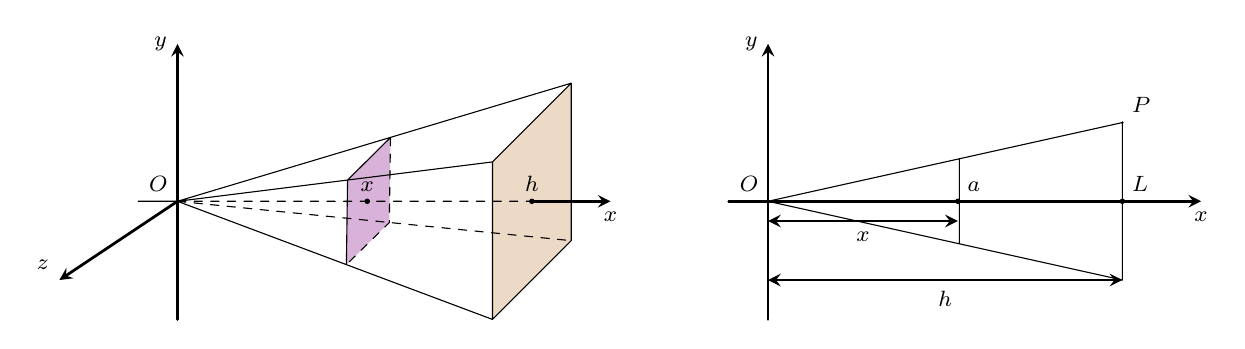
\begin{tikzpicture}[scale=.5, font=\footnotesize, line join=round, line cap=round, >=stealth]
				\begin{scope}[shift={(0,0)}]
					\fill[brown!30] (8,1)--(10,3)--(10,-1)--(8,-3)--cycle;
					\fill[violet!30] (5.41,1.62)--(5.38,-0.54)--(4.29,-1.61)--(4.32,0.54)--cycle;
					\draw[->,line width = 1pt] (9,0)--(11,0) node[below]{$x$};
					\draw[->,line width = 1pt] (0,-3)--(0,4) node[left]{$y$};
					\draw[->,line width = 1pt] (0,0)--(-3,-2) node[above left]{$z$};
					\draw (8,1)--(10,3)--(10,-1)--(8,-3)--cycle	(4.29,-1.61)--(4.32,0.54)--(5.41,1.62)	(0,0)--(8,-3)	(0,0)--(8,1)	(0,0)--(10,3)	(-1,0)--(0,0);	
					\draw[dashed] (5.41,1.62)--(5.38,-0.54)--(4.29,-1.61)	(0,0)--(10,-1)	(0,0)--(9,0);
					\fill (0,0) circle (1pt) node[above left]{$O$};
					\fill (4.82,0) circle (2pt) node[above]{$x$};
					\fill (9,0) circle (2pt) node[above]{$h$};
				\end{scope}
				\begin{scope}[shift={(15,0)}]
					\draw[->,line width = 1pt] (-1,0)--(11,0) node[below]{$x$};
					\draw[->,line width = 1pt] (0,-3)--(0,4) node[left]{$y$};
					\draw (0,0)--(9,2)--(9,-2)--cycle	(4.86,1.08)--(4.86,-1.08);
					\fill (4.82,0) circle (2pt) node[above right]{$a$};
					\fill (9,0) circle (2pt) node[above right]{$L$};
					\draw[<->,line width = 1pt] (0,-0.5)--(4.82,-0.5) node[pos=0.5,sloped,below]{$x$};
					\draw[<->,line width = 1pt] (0,-2)--(9,-2) node[pos=0.5,sloped,below]{$h$};
					\fill (0,0) circle (1pt) node[above left]{$O$};
					\fill (9,2) circle (1pt) node[above right]{$P$};
				\end{scope}
			\end{tikzpicture}
		\end{center}
		\begin{center}
			Hình $4.23$
		\end{center}
		Chọn trục $Ox$ sao cho gốc $O$ trùng với đỉnh của khối chóp và trục đi qua tâm của đáy. Khi đó, đáy của khối chóp nằm trên mặt phẳng vuông góc với $Ox$ tại $x=h$.\\
		Mỗi mặt phẳng vuông góc với trục $Ox$ tại điểm có hoành độ bằng $x(0 \leq x \leq h)$, cắt khối chóp theo mặt cắt là hình vuông có cạnh là $a$.\\
		Theo định lí Tha-les, ta có $\dfrac{x}{h}=\dfrac{\frac{a}{2}}{\frac{L}{2}}$, suy ra $a=\dfrac{L}{h} x$.\\
		Do đó, diện tích của mặt cắt này là $S(x)=\dfrac{L^2}{h^2} x^2$.\\
		Vậy thể tích của khối chóp này là $V=\displaystyle\int_0^h S(x) \mathrm{\,d} x=\displaystyle\int_0^h \dfrac{L^2}{h^2} x^2 \mathrm{~d}x=\left.\dfrac{L^2}{h^2} \dfrac{x^3}{3}\Bigg|_0^h \right. =\dfrac{1}{3} L^2h$.
	}
\end{bt}

\begin{bt}%[2D4H3-3]
% nguon: Archive/2024/0. [LVH] BG - 12 New - 4in1-20240625T224301Z-001/0. [LVH] BG - 12 New - 4in1/2. [LVH] TEX SGK 12 NEW-20240418T074833Z-001/2. [LVH] TEX SGK 12 NEW/[LVH] SGK-12-KNTT/data/C4/12-c4-bai13-ungdunghinhhoccuatichphan.tex #1165
%[TeX hóa SGK KNTT 12]%[Anh Hoàng Lê]
	Tính thể tích khối tròn xoay sinh ra khi quay quanh trục $Ox$ hình phẳng giới hạn bởi đồ thị hàm số $y=\sqrt{x}$, trục hoành và hai đường thẳng $x=0$, $x=1$ (Hình $4.26$).
	\begin{center}
		\begin{tikzpicture}[scale=1.5, font=\footnotesize, line join=round, line cap=round, >=stealth]
			% Scope 1
			\begin{scope}[shift={(0,0)}]
				\fill[blue!20, domain=0:2, variable=\x]
				(0,0) -- plot ({\x},{sqrt(\x)}) -- (2,0) -- cycle;
				\draw[->] (-0.5,0) -- (2.5,0) node[right] {$x$};
				\foreach \x/\xtext in {1/x,2/1}
				\draw (\x cm,1pt) -- (\x cm,-1pt) node[anchor=north] {$\xtext$};
				\draw[->] (0,-0.5) -- (0,1.5) node[above] {$y$};
				\foreach \y/\ytext in {}
				\draw (1pt,\y cm) -- (-1pt,\y cm) node[anchor=east] {$\ytext$};
				\draw[domain=0:2,smooth,variable=\x,blue] plot ({\x},{sqrt(\x)});
				\draw[red] (1,1)--(1,0) ;
				\draw[-{Stealth[length=3mm,width=3mm]}] (3,0.5) -- (4.5,0.5);
				\fill (0,0) circle (1pt) node[below left]{$O$};
			\end{scope}
			% Scope 2
			\begin{scope}[shift={(6,0)}]
				\fill[blue!20, domain=0:2, variable=\x]
				(0,0) -- plot ({\x},{sqrt(\x)}) -- (2,0) -- cycle;
				\fill[blue!20,domain=0:2,variable=\x]
				(0,0) -- plot ({\x},{-sqrt(\x)}) -- (2,0) -- cycle;
				\fill[yellow!20] (1,0) ellipse (0.15cm and 1cm);
				\draw[->] (2,0) -- (2.5,0) node[right] {$x$};
				\foreach \x/\xtext in {1/,2/}
				\draw (\x cm,1pt) -- (\x cm,-1pt) node[anchor=north] {$\xtext$};
				\draw[->] (0,-1.5) -- (0,1.5) node[above] {$y$};
				\foreach \y/\ytext in {}
				\draw (1pt,\y cm) -- (-1pt,\y cm) node[anchor=east] {$\ytext$};
				\draw[domain=0:2,smooth,variable=\x,blue] plot ({\x},{sqrt(\x)});
				\draw[domain=0:2,smooth,variable=\x,blue] plot ({\x},{-sqrt(\x)});
				\fill (2,0) circle (0pt) node[below right]{$1$};
				\draw (2,0) ellipse (0.35cm and 1.41cm);
				\draw (2,1.41)--(2,-1.41)	(-0.5,0)--(0,0);
				\draw[dashed] (0,0)--(2,0);
				\fill (0,0) circle (1pt) node[below left]{$O$};
				\draw[dashed,rotate=-90] (1,1) arc (0:180:1cm and 0.15cm); 
				\draw[rotate=90] (1,-1) arc (0:180:1cm and 0.15cm); 
			\end{scope}
		\end{tikzpicture}
	\end{center}
	\begin{center}
		Hình $4.26$
	\end{center}
	\loigiai{
		Thể tích khối tròn xoay cần tính là
		$$
		V=\pi \displaystyle\int_0^1f^2(x) \mathrm{\,d} x=\pi \displaystyle\int_0^1(\sqrt{x})^2 \mathrm{~d}x=\pi \displaystyle\int_0^1x \mathrm{~d}x=\left.\dfrac{\pi x^2}{2}\right|_0^1=\dfrac{\pi}{2}.
		$$
	}
\end{bt}

\begin{bt}%[2D4H3-3]
% nguon: Archive/2024/0. [LVH] BG - 12 New - 4in1-20240625T224301Z-001/0. [LVH] BG - 12 New - 4in1/2. [LVH] TEX SGK 12 NEW-20240418T074833Z-001/2. [LVH] TEX SGK 12 NEW/[LVH] SGK-12-KNTT/data/C4/12-c4-bai13-ungdunghinhhoccuatichphan.tex #1166
%[TeX hóa SGK KNTT 12]%[Anh Hoàng Lê]
	Tính thể tích của khối cầu bán kính $R$.
	\loigiai{
		\immini{Khối cầu bán kính $R$ có thể xem là vật thể sinh ra khi quay quanh trục hoành nửa hình tròn giới hạn bởi đồ thị hàm số $y=\sqrt{R^2-x^2}\,(-R \leq x \leq R)$, trục hoành và hai đường thẳng $x=-R$, $x=R$ (Hình $4.27$).\\
			Do đó, thể tích của khối cầu bán kính $R$ là
			\begin{eqnarray*}
				V & = & \pi \displaystyle\int_{-R}^R\left(\sqrt{R^2-x^2}\right)^2 \mathrm{~d}x=\pi \displaystyle\int_{-R}^R\left(R^2-x^2\right) \mathrm{\,d} x \\
				&=& \left.\pi\left(R^2x-\dfrac{x^3}{3}\right)\right|_{-R}^R=\dfrac{4}{3} \pi R^3.
		\end{eqnarray*}}
		{\begin{tikzpicture}[scale=0.8, font=\footnotesize, line join=round, line cap=round, >=stealth]
				\path (0.5,-4)node[below]{Hình $4.27$};
				\filldraw[blue!20] (3,0) arc [start angle=0, end angle=180, radius=3];
				\draw (0,0)circle(1pt) node[below left]{$O$};
				\draw[->] (-4,0) -- (4.6,0) node[below]{$x$};
				\draw[->] (0,-4) -- (0,4) node[left]{$y$};
				\draw (3,0) arc [start angle =0, end angle =180, radius=3];
				\draw[dashed] (-3,0) arc [start angle =180, end angle =360, radius=3];
				\draw[dashed] (0,0) ellipse [x radius =0.7, y radius=3];
				\fill[ fill=black,pattern=north east lines,pattern color=black] (2,0) ellipse [x radius=0.45, y radius=2.2];
				\draw[dashed] (2,0) ellipse [x radius=0.45, y radius=2.2];
				%\draw (2,0)circle(1pt)node[below]{$x$}--(2,2.2)node[above right]{$y=\sqrt{R^2-x^2}$};
				\draw[->,>=Stealth] ($(3.9,0.3)+(0:0)$)node[below]{} arc (90:370:{0.1} and {0.5});
				\path (-3,0)node[below left]{$-R$} (3,0)node[below right]{$R$};
		\end{tikzpicture}}
	}
\end{bt}

\begin{bt}%[2D4H3-3]
% nguon: Archive/2024/0. [LVH] BG - 12 New - 4in1-20240625T224301Z-001/0. [LVH] BG - 12 New - 4in1/2. [LVH] TEX SGK 12 NEW-20240418T074833Z-001/2. [LVH] TEX SGK 12 NEW/[LVH] SGK-12-KNTT/data/C4/12-c4-bai13-ungdunghinhhoccuatichphan.tex #1167
%[TeX hóa SGK KNTT 12]%[Anh Hoàng Lê]
	Tính thể tích của khối tròn xoay sinh ra khi quay hình phẳng giới hạn bởi các đường sau xung quanh truc $Ox\colon$$y=2x-x^2$, $y=0$, $x=0$, $x=2$.
	\loigiai{
		Thể tích của khối tròn xoay là
		$$V=\pi \displaystyle\int_0^2 \left(2x-x^2 \right)^2 \mathrm{\,d} x
		= \pi \displaystyle\int_0^2 \left(x^4-4x^3+4x^2\right) \mathrm{\,d} x
		=\left.\pi\left(\dfrac{x^5}{5}-x^4+\dfrac{4}{3}x^3\right)\right|_0^2
		=\dfrac{16}{15}\pi.$$
	}
\end{bt}

\begin{bt}%[2D4H3-3]
% nguon: Archive/2024/0. [LVH] BG - 12 New - 4in1-20240625T224301Z-001/0. [LVH] BG - 12 New - 4in1/2. [LVH] TEX SGK 12 NEW-20240418T074833Z-001/2. [LVH] TEX SGK 12 NEW/[LVH] SGK-12-KNTT/data/C4/12-c4-bai13-ungdunghinhhoccuatichphan.tex #1168
%[TeX hóa SGK KNTT 12]%[Anh Hoàng Lê]
	Khối chỏm cầu có bán kính $R$ và chiều cao $h(0<h \leq R)$ sinh ra khi quay hình phẳng giới hạn bởi cung tròn có phương trình $y=\sqrt{R^2-x^2}$, trục hoành và hai đường thẳng $x=R-h$, $x=R$ xung quanh trục $Ox$ (Hình $4.30$). Tính thể tích của khối chỏm cầu này.
	\begin{center}
		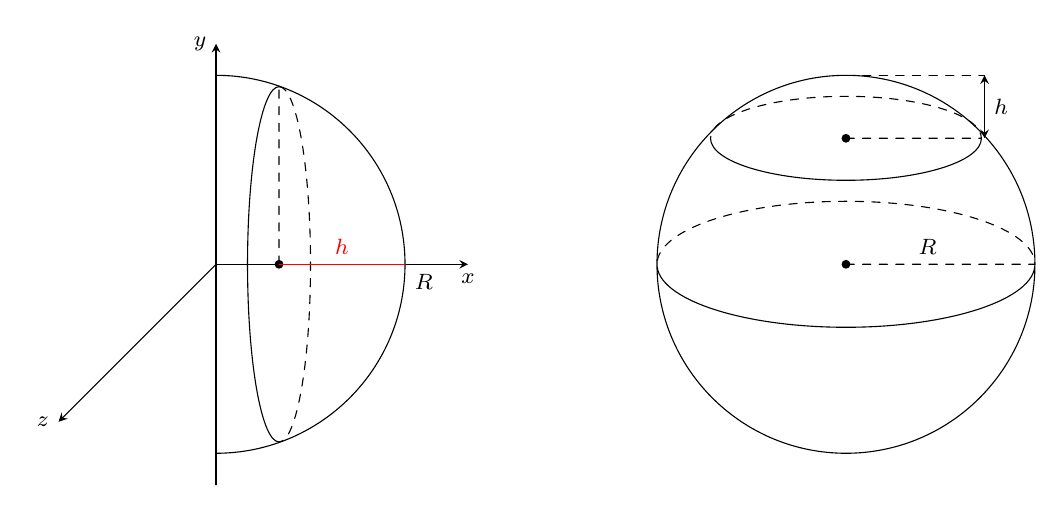
\begin{tikzpicture}[scale=.8, font=\footnotesize, line join=round, line cap=round, >=stealth]
			% Vẽ hình thứ nhất
			\begin{scope}[shift={(0,0)}]
				\draw[->] (0,0) -- (4,0) node[below] {$x$};
				\draw[->] (0,-3.5) -- (0,3.5) node[left] {$y$};
				\draw[->] (0,0) -- (-2.5,-2.5) node[left] {$z$};
				\draw (0,-3) arc (-90:90:3cm and 3cm);
				\draw[dashed] (1,2.82) arc (90:-90:0.5cm and 2.82cm)	(1,0)--(1,2.82);
				\draw (1,2.82) arc (90:270:0.5cm and 2.82cm);
				\fill (3,0) circle (0pt) node[below right]{$R$};
				\fill (1,0) circle (2pt) ;
				\draw[red]	(1,0)--(3,0) node[pos=0.5,sloped,above]{$h$};
				
			\end{scope}
			% Vẽ hình thứ hai
			\begin{scope}[shift={(10,0)}] 
				\def\R{3} % Bán kính
				\coordinate (O) at (0,0);
				\coordinate (O') at (0,2);
				\coordinate (A) at (\R,0);
				\draw (O) circle (\R) (A) arc (0:-180: {\R} and {\R/3});
				\draw[dashed] (O)--(A) arc (0:180: {\R} and {\R/3});
				\draw  (2.15,2) arc (0:-180: {2.15} and {2/3});
				\draw[dashed] (0,2)--(2.15,2) arc (0:180: {2.15} and {2/3});
				\draw[dashed] (0,3)--(2.2,3) ;
				\draw[<->] 	(2.2,2)--(2.2,3) node[pos=0.5,right]{$h$};
				\foreach \diem in {O,O'}	\fill (\diem)circle(2pt);
				\fill (1,0) circle (0pt) node[above right]{$R$};	
			\end{scope}
		\end{tikzpicture}
	\end{center}
	\begin{center}
		Hình $4.30$
	\end{center}
	\loigiai{
		Thể tích khối chỏm cầu là
		\begin{eqnarray*}
			V &=&\pi \displaystyle\int_{R-h}^{R} y^2(x) \mathrm{\,d}x=\pi \displaystyle\int_{R-h}^{R}\left(R^2-x^2\right) \mathrm{\,d}x \\
			& = &\left.\pi\left(R^2 x-\dfrac{x^3}{3}\right)\right|_{R-h}^{R} \\
			& =&\pi\left[R^3-\dfrac{R^3}{3}-R^2(R-h)+\dfrac{(R-h)^3}{3}\right] \\
			& =&\pi h^2\left(R-\dfrac{h}{3}\right).
		\end{eqnarray*}
	}
\end{bt}

\begin{bt}%[2D4V3-3]
% nguon: Archive/2024/0. [LVH] BG - 12 New - 4in1-20240625T224301Z-001/0. [LVH] BG - 12 New - 4in1/2. [LVH] TEX SGK 12 NEW-20240418T074833Z-001/2. [LVH] TEX SGK 12 NEW/[LVH] SGK-12-KNTT/data/C4/12-c4-bai13-ungdunghinhhoccuatichphan.tex #1169
%[TeX hóa SGK KNTT 12]%[Anh Hoàng Lê]
	Cho tam giác vuông $OAB$ có cạnh $OA=$ a nằm trên trục $Ox$ và $\widehat{AOB}=\alpha\left(0<\alpha \leq \dfrac{\pi}{4}\right)$. Gọi $\mathcal{B}$ là khối tròn xoay sinh ra khi quay miền tam giác $OAB$ xung quanh trục $Ox$ (Hình $4.31$).
	\begin{enumerate}
		\item  Tính thể tích $V$ của $\mathcal{B}$ theo $a$ và $\alpha$.
		\item  Tìm $\alpha$ sao cho thể tích $V$ lớn nhất.
	\end{enumerate}
	\begin{center}
		\begin{tikzpicture}[scale=1, font=\footnotesize, line join=round, line cap=round, >=stealth]
			\fill[yellow!30]	(0,0)--(4,2)--(4,0)--cycle;
			\draw[->] (4,0) -- (5.5,0) node[right] {$x$};
			\draw[->] (0,-2.5) -- (0,2.5) node[above] {$y$};
			\draw[->] (0,0) -- (-1.5,-1.5) node[below left] {$z$};
			\draw (0,0)--(4,2)	(0,0)--(4,-2)	(4,2)--(4,0)	(-0.5,0)--(0,0);
			\draw[dashed] (0,0)--(4,0)	;
			\draw (4,0) ellipse (0.5 and 2);
			\fill (0,0) circle (1pt) node[above left]{$O$};
			\fill (4,0) circle (1pt) node[below]{$A$};
			\fill (4,2) circle (1pt) node[above]{$B$};
			\clip (4,0) -- (0,0) -- (4,2);
			\draw (0,0) circle (1cm);
			\draw ($(0,0)+(1,0)$) node[above right]{$\alpha$};
			\node[below] at (2.5,-2.5) {Hình $4.31$};
		\end{tikzpicture}
	\end{center}
	\loigiai{
		\begin{enumerate}
			\item Phương trình đường thẳng $OB$ là $y=x \tan \alpha$.\\
			Thể tích $V$ của $\mathcal{B}$ là
			$$
			V=\pi \displaystyle\int_0^a y^2\mathrm{\,d} x=\pi \displaystyle\int_0^a x^2 \tan^2 \alpha \mathrm{\,d} x=\left.\pi \tan^2 \alpha \cdot \dfrac{x^3}{3}\right|_0^{a}=\pi \tan^2 \alpha \cdot \dfrac{a^3}{3}.
			$$
			\item 
			Đặt $OB=R \Rightarrow OA=a=R \cos \alpha $. Khi đó $V=\dfrac{\pi R^3}{3}\left(\cos \alpha-\cos^3 \alpha \right)$.\\
			Đặt $t=\cos \alpha \Rightarrow t \in\left[\dfrac{\sqrt{2}}{2};1\right)$ (vì $\alpha \in\left(0;\dfrac{\pi}{4}\right]$ ). Ta có $V=\dfrac{\pi R^3}{3}\left(t-t^3\right)$
			$$
			V'=\dfrac{\pi R^3}{3}\left(1-3t^2\right), V'=0 \Leftrightarrow \hoac{&
				t=\dfrac{1}{\sqrt{3}} \\
				& t=-\dfrac{1}{\sqrt{3}}} \text{(Loại)}
			$$
			Ta tính được $V\left( \dfrac{\sqrt{2}}{2} \right)=\dfrac{\sqrt{2}R^3}{12}; \,\,
			V\left( 1 \right)=0$.\\
			Vậy $\max _{\left(0;\dfrac{\pi}{4}\right]} V(\alpha)=\max _{\left[\dfrac{\sqrt{2}}{2};1\right)} V(t)=V\left(\dfrac{\sqrt{2}}{2}\right)=\dfrac{\sqrt{2}R^3}{12}$.\\(trong đó $\cos \alpha=\dfrac{\sqrt{2}}{2} \Rightarrow \alpha=45^{\circ}$).
		\end{enumerate}
	}
\end{bt}

\begin{bt}%[2D3H2-2]
% nguon: Archive/2024/TaiLieuGiangDay/3. K12 - 4in1 - Thongke/data/4. Bai2-Dang1-PhuongSai,Dolechchuan.tex #1918
[Mức độ 2-CTST]
Hãy tính phương sai của mẫu số liệu ghép nhóm sau
\begin{center}
\begin{tabular}{|c|c|c|c|c|c|}
\hline Chiều cao (cm) &{$[160;164)$} &{$[164;168)$} &{$[168;172)$} &{$[172;176)$} &{$[176;180)$} \\
\hline Số học sinh & $ 3 $ & $ 5 $ & $ 8 $ & $ 4 $ & $ 1 $ \\
\hline
\end{tabular}
\end{center}
\loigiai{
Ta có bảng sau
\begin{center}
\begin{tabular}{|c|c|c|c|c|c|}
\hline Chiều cao (cm) &{$[160;164)$} &{$[164;168)$} &{$[168;172)$} &{$[172;176)$} &{$[176;180)$} \\
\hline Giá trị đại diện & $ 162 $ & $ 166 $ & $ 170 $ & $ 174 $ & $ 178 $ \\
\hline Số học sinh & $ 3 $ & $ 5 $ & $ 8 $ & $ 4 $ & $ 1 $ \\
\hline
\end{tabular}
\end{center}
Ta có cỡ mẫu $ n=21 $.\\
Số trung bình của mẫu số liệu ghép nhóm là
$$ \overline{x}=\dfrac{3\cdot162+5\cdot166+8\cdot170+4\cdot174+1\cdot178}{21}=\dfrac{3550}{21}. $$
Phương sai của mẫu số liệu ghép nhóm là  $$ S^2=\dfrac{1}{21}(3\cdot162^2+5\cdot166^2+8\cdot170^2+4\cdot174^2+1\cdot178^2)-\left(\dfrac{3550}{21} \right)^2\approx18{,}14.  $$
}
\end{bt}

\begin{bt}%[2D3H2-2]
% nguon: Archive/2024/TaiLieuGiangDay/3. K12 - 4in1 - Thongke/data/4. Bai2-Dang1-PhuongSai,Dolechchuan.tex #1919
[Mức độ 2-CTST]
Cân nặng của một số quả mít trong một khu vườn được thống kê ở bảng sau
\begin{center}
\begin{tabular}{|c|c|c|c|c|c|}
\hline \begin{tabular}{c}
\textbf{Cân nặng (kg)}
\end{tabular} &{$[4; 6)$} &{$[6; 8)$} &{$[8; 10)$} &{$[10; 12)$} &{$[12; 14)$} \\
\hline \textbf{Số quả mít} & 6 & 12 & 19 & 9 & 4 \\
\hline
\end{tabular}
\end{center}
Hãy tính phương sai của mẫu số liệu ghép nhóm trên. (Kết quả các phép tính làm tròn đến hàng phần trăm).
\loigiai{
Ta có bảng thống kê cân nặng của các quả mít theo giá trị đại diện
\begin{center}
\begin{tabular}{|c|c|c|c|c|c|}
\hline \begin{tabular}{c}
\textbf{Cân nặng đại diện (kg)}
\end{tabular} &{$5$} &{$7$} &{$9$} &{$11$} &{$13$} \\
\hline \textbf{Số quả mít} & 6 & 12 & 19 & 9 & 4 \\
\hline
\end{tabular}
\end{center}
Cỡ mẫu $ n=6+12+19+9+4=50 $.\\
Số trung bình của mẫu số liệu ghép nhóm là
$$ \overline{x}=\dfrac{6\cdot 5+12\cdot7+19\cdot9+9\cdot11+4\cdot13}{50}=8{,}72. $$
Phương sai của mẫu số liệu ghép nhóm là
$$ S^2=\dfrac{1}{50}\left(6\cdot5^2+12\cdot 7^2+19\cdot9^2+9\cdot11^2+4\cdot13^2 \right)-8{,}72^2\approx4{,}80.  $$
}
\end{bt}

\begin{bt}%[2D4C3-5]
% nguon: Archive/2024/TaiLieuGiangDay/5.HH Oxyz/VDC_TDM.tex #3154
%[Anh Tuấn]
	Cho một bình ban đầu chưa đựng gì có dạng hình chóp cụt đều có đáy dưới nhỏ hơn là hình vuông có cạnh bằng $30\,\mathrm{cm}$, đáy trên có cạnh bằng $60\,\mathrm{cm}$, chiều cao bằng $100\,\mathrm{cm}$. 
	Dùng một vòi cho chảy nước vào bình này với lưu lượng không đổi $2000\,\text{cm$^3$/phút}$. 
	Trong bài toán, đơn vị thể tích tính theo $\mathrm{cm^3}$ và đơn vị dài tính theo $\mathrm{cm}$, đơn vị thời gian tính theo phút, các kết quả đều được làm tròn đến hàng phần mười.
	Hãy xây dựng hoặc tìm cách xác định hàm biểu diễn tốc độ dâng của chiều cao mực nước trong bình?
		\begin{center}
		\begin{tikzpicture}[scale=0.8,font=\footnotesize, line join=round, line cap=round, >=stealth]
			\def\a{3} \def\aa{5} 
			\def\b{2} \def\bb{3.5}
			\def\h{5}
			\path (0:0) coordinate (A)
			++(0:\a) coordinate (D)
			++(-150:\b) coordinate (C)
			($(A)+(C)-(D)$) coordinate (B)
			($(A)+(90:\h)$) coordinate (A')
			++(0:\aa) coordinate (D')
			++(-150:\bb) coordinate (C')
			($(A')+(C')-(D')$) coordinate (B')
			($(C)!0.5!(D)$) coordinate (M)
			($(C')!0.5!(D')$) coordinate (N)
			($(M)+(4.3,0)$) coordinate (M')
			($(N)+(3,0)$) coordinate (N')
			;
			\fill[gray!30] (A)--(B)--(C)--(D)--(A);
			\draw[dashed] 	(B)--(A)--(D)	(A)--(A') (M)--(M') (N)--(N');
			\draw 	(C)--(C') (D)--(D') 	(B)--(B')(C)--(C')(B)--(C)--(D) 
			(A')--(B')--(C')--(D')--cycle;
			\draw [<->] (N')--(M') node[midway, left]{$100$ cm} ;
%			\foreach \x/\g in {A/160,B/-135,C/-45,D/0,A'/90,B'/135,C'/90,D'/45}
%			\fill (\x) circle (1pt)
%			($(\g:3mm)+(\x)$) node {$\x$};
			\fill (A') -- (D') node[midway, above]{$60$ cm} (B) -- (C) node[midway, below]{$30$ cm};	
		\end{tikzpicture}
	\end{center}
	\loigiai{
	Gọi $h$ (cm) là chiều cao của mực nước tại thời điểm $t$ (phút).\\
	Vì hình chóp cụt đều có tiết diện là hình vuông, và cạnh của nó tăng đều từ $30$ cm lên $60$ cm theo chiều cao từ $0$ đến $100$ cm nên độ dài cạnh của tiết diện tại độ cao $h$ là
	\[
	a = 30 + \frac{60 - 30}{100} \cdot h = 30 + 0{,}3h~\text{(cm)}.
	\]
	Diện tích mặt cắt ngang tại độ cao $h$ là
	\[
	S(h) = a^2 = \left(30 + 0{,}3h\right)^2~\left(\text{cm$^2$} \right).
	\]
	Thể tích nước đến độ cao $h$ là
	\begin{eqnarray*}
		V(h) &=& \displaystyle\int_0^h S(x)\, dx = \int_0^h \left(30 + 0{,}3x\right)^2 dx\\
		&=& \displaystyle\int_0^h \left(900 + 18x + 0{,}09x^2\right) dx \\
		&=& 900h + 9h^2 + 0{,}03h^3~\left(\text{cm$^3$} \right).
	\end{eqnarray*}
	Vì vòi nước chảy vào bình này với lưu lượng không đổi $2000\,\text{cm$^3$/phút}$ nên tốc độ dâng của chiều cao mực nước trong bình là
	\[\dfrac{2000}{V'(h)}=\dfrac{2000}{900 + 18h + 0{,}09h^2}.\]
	}
	Vậy hàm biểu diễn tốc độ dâng của chiều cao mực nước trong bình là $f(h)=\dfrac{2000}{900 + 18h + 0{,}09h^2}$ (cm/phút).
\end{bt}

\begin{bt}%[2D4V3-1]
% nguon: Archive/2024/TaiLieuGiangDay/5.HH Oxyz/VDC_TDM.tex #3157

	Cho hai hình phẳng $\left(H_1\right)$ và $\left(H_2\right)$ được tô màu như hình vẽ bên dưới. Biết các điểm $A$, $B$, $C$, $D$, $E$ đều là các đỉnh của các đường parabol. Hãy tính diện tích các hình phẳng $\left(H_1\right)$ và $\left(H_2\right)$?	
	\begin{center}
		\begin{tikzpicture}[scale=.45, font=\footnotesize, line join=round, line cap=round, >=stealth]		
			\def\xmin{-8}\def\xmax{8}\def\ymin{-4.5}\def\ymax{13}						
			\begin{scope}
				[rotate=-90]		
				\clip (\xmin,\ymin) rectangle (7,\ymax);
				\fill[gray!30] plot[shift={(-5,0)},smooth,samples=200,domain=-2:0] (\x,{-1*((\x)^2)+0*\x+4})
				--plot[shift={(-2.5,4)},smooth,samples=200,domain=-2.5:0] (\x,{-.64*((\x)^2)+0*\x+4})
				-- plot[shift={(0,8)},smooth,samples=200,domain=-2.5:2.5] (\x,{-.64*((\x)^2)+0*\x+4})
				--plot[shift={(2.5,4)},smooth,samples=200,domain=0:2.5] (\x,{-.64*((\x)^2)+0*\x+4})	
				--plot[shift={(5,0)},smooth,samples=200,domain=0:2] (\x,{-1*((\x)^2)+0*\x+4});
				\draw[shift={(5,0)},smooth,samples=200,domain=-2:2] plot (\x,{-1*((\x)^2)+0*\x+4});	%1
				
				\draw[name path=a2,shift={(-5,0)},smooth,samples=200,domain=-2:2] plot (\x,{-1*((\x)^2)+0*\x+4});	%2
				
				\draw[name path=a3,smooth,samples=200,domain=-3:3] plot (\x,{-4/9*((\x)^2)+0*\x+4});	%3
				
				\draw[name path=a4,shift={(2.5,4)},smooth,samples=200,domain=-2.5:2.5] plot (\x,{-.64*((\x)^2)+0*\x+4});	
				%4
				\draw[name path=a5,shift={(-2.5,4)},smooth,samples=200,domain=-2.5:2.5] plot (\x,{-.64*((\x)^2)+0*\x+4});	 %5
				\draw[name path=a6,shift={(0,8)},smooth,samples=200,domain=-2.5:2.5] plot (\x,{-.64*((\x)^2)+0*\x+4});
				
				\draw (-7,0)rectangle (7,12);			
				
				\foreach \x in {-5,-3,...,5}
				\draw[dashed] (\x,0)--(\x,12);				
				\foreach \x in {4,8}
				\draw[dashed] (-7,\x)--(7,\x);			
				
				\fill (-5,4) node[above right]{$A$} circle (1.5pt)
				(0,4) node[left]{$B$} circle (1.5pt)
				(5,4) node[below right]{$C$} circle (1.5pt)
				(-2.5,8) node[left]{$D$} circle (1.5pt)
				(2.5,8) node[left]{$E$} circle (1.5pt)
				; 
				
				\draw[|<->|,blue] (-7,-.75)--node[black,midway,sloped,fill=white]{$2$}(-5,-.75);
				
				\draw[|<->|,blue] (-7.65,0)--node[black,midway,sloped,fill=white]{$4$}(-7.65,4);	
				
				
				\draw (-2.5,3.5) node[]{$(H_1)$};		
			\end{scope}				
			\end{tikzpicture}			
			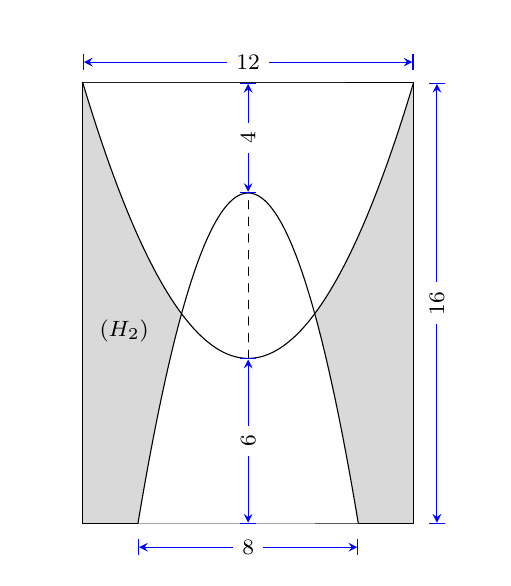
\begin{tikzpicture}[scale=.35, font=\footnotesize, line join=round, line cap=round, >=stealth]			
				\def\xmin{-8}\def\xmax{9.5}\def\ymin{-1.25}\def\ymax{18}
				\clip (\xmin,\ymin) rectangle (8.5,\ymax);					
				\draw[fill=gray!30] (-6,0)rectangle (6,16);				
				\fill[smooth,samples=200,domain=-4:4, white] plot (\x,{-.75*((\x)^2)+0*\x+12});	
				\fill[smooth,samples=200,domain=-6:6,white] plot (\x,{5/18*((\x)^2)+0*\x+6});	
				\draw[smooth,samples=200,domain=-4:4] plot (\x,{-.75*((\x)^2)+0*\x+12});	
				\draw[smooth,samples=200,domain=-6:6] plot (\x,{5/18*((\x)^2)+0*\x+6});		
				\draw[|<->|,blue] (-6,16.75)--node[black,midway,sloped,fill=white]{$12$}(6,16.75);
				\draw[|<->|,blue] (6.85,0)--node[black,midway,sloped,fill=white]{$16$}(6.85,16);	
				\draw[|<->|,blue] (-4,-.85)--node[black,midway,sloped,fill=white]{$8$}(4,-.85);				
				\draw[|<->|,blue] (0,0)--node[black,midway,sloped,fill=white]{$6$}(0,6);
				\draw[|<->|,blue] (0,12)--node[black,midway,sloped,fill=white]{$4$}(0,16);				
				\draw[dashed] (0,6)--(0,12);
				\draw (-4.5,7) node[]{$(H_2)$};
			\end{tikzpicture}
	\end{center}
	\loigiai{Không mất tỉnh tổng quát, vẽ lại hình $(H_1)$ như bên dưới. 
	\begin{center}
		\begin{tikzpicture}[scale=.45, font=\footnotesize, line join=round, line cap=round, >=stealth]
			
			\def\xmin{-8}\def\xmax{10}\def\ymin{-2.5}\def\ymax{13}						
			\begin{scope}
				%[rotate=-90]		
				\clip (\xmin,-2) rectangle (8,\ymax);
				\fill[gray!30] plot[shift={(-5,0)},smooth,samples=200,domain=-2:0] (\x,{-1*((\x)^2)+0*\x+4})
				--plot[shift={(-2.5,4)},smooth,samples=200,domain=-2.5:0] (\x,{-.64*((\x)^2)+0*\x+4})
				-- plot[shift={(0,8)},smooth,samples=200,domain=-2.5:2.5] (\x,{-.64*((\x)^2)+0*\x+4})
				--plot[shift={(2.5,4)},smooth,samples=200,domain=0:2.5] (\x,{-.64*((\x)^2)+0*\x+4})	
				--plot[shift={(5,0)},smooth,samples=200,domain=0:2] (\x,{-1*((\x)^2)+0*\x+4});
				\draw[shift={(5,0)},smooth,samples=200,domain=-2:2] plot (\x,{-1*((\x)^2)+0*\x+4});	%1
				
				\draw[name path=a2,shift={(-5,0)},smooth,samples=200,domain=-2:2] plot (\x,{-1*((\x)^2)+0*\x+4});	%2
				
				\draw[name path=a3,smooth,samples=200,domain=-3:3] plot (\x,{-4/9*((\x)^2)+0*\x+4});	%3
				
				\draw[name path=a4,shift={(2.5,4)},smooth,samples=200,domain=-2.5:2.5] plot (\x,{-.64*((\x)^2)+0*\x+4});	
				%4
				\draw[name path=a5,shift={(-2.5,4)},smooth,samples=200,domain=-2.5:2.5] plot (\x,{-.64*((\x)^2)+0*\x+4});	 %5
				\draw[name path=a6,shift={(0,8)},smooth,samples=200,domain=-2.5:2.5] plot (\x,{-.64*((\x)^2)+0*\x+4});
				
				\draw (-7,0)rectangle (7,12);			
				
				\foreach \x in {-5,-3,...,5}
				\draw[dashed] (\x,0)--(\x,12);				
				\foreach \x in {4,8}
				\draw[dashed] (-7,\x)--(7,\x);			
				
				\fill (-5,4) node[above left]{$A$} circle (1.5pt)
				(0,4) node[below]{$B$} circle (1.5pt)
				(5,4) node[above right]{$C$} circle (1.5pt)
				(-2.5,8) node[below]{$D$} circle (1.5pt)
				(2.5,8) node[below]{$E$} circle (1.5pt)
				; 
				
				\draw[|<->|,blue] (-7,-1.25)--node[black,midway,sloped,fill=white]{$2$}(-5,-1.25);
				
				\draw[|<->|,blue] (-7.65,0)--node[black,midway,sloped,fill=white]{$4$}(-7.65,4);				
				
				\draw (-2.5,3.5) node[]{$(H_1)$};
				
				\fill (-7,0) node[below]{$M$} circle (1.5pt)
				(7,0) node[below]{$N$} circle (1.5pt)
				(7,4) node[above right]{$I$} circle (1.5pt)
				(-7,4) node[above left]{$K$} circle (1.5pt)
				
				(-5,8) node[above left]{$G$} circle (1.5pt)
				(5,8) node[above right]{$R$} circle (1.5pt)
				(5,0) node[below]{$O_1$} circle (1.5pt)
				(2.5,4) node[below]{$O_2$} circle (1.5pt)
				;						
			\end{scope}				
		\end{tikzpicture}			
	\end{center}
	
	\begin{itemize}
		\item Tính diện tích hình $(H_1)$.
		Từ hình vẽ ta thấy hai hình parabol ở dưới cùng bằng nhau. Do đó chọn hệ trục tọa độ $Oxy$ sao cho $Ox$ trùng với tia $O_1N$ và $Oy$ trùng với tia $OC$. Khi đó ta có $N(2,0)$ và $C(0,4)$.\\
		Parabol đi qua điểm $C$ và $N$ có phương trình là $y=-x^2+4$.\\
		Do đó diện tích phân tô đậm trong hình chữ nhật $MNIK$ là $$S_1=S_{MNIK}-2\displaystyle\int\limits_0^2[4-(-x^2+4)]\mathrm{\,d}x=4\cdot 14-2\cdot \dfrac{8}{3}=\dfrac{152}{3}.$$
		Từ dữ liệu hình vẽ ba hình parabol ở trên bằng nhau. Chọn hệ trục tọa độ $Oxy$ sao cho $O$ trùng với trung điểm $O_2$ của $BC$, trục $Ox$ trùng với tia $O_2C$ và trục $Oy$ trùng với tia $O_2E$. Khi đó ta có $C(2{,}5;0)$ và $E(0;4)$. \\
		Parabol đi qua điểm $E$ và $C$ có phương trình là $y=-\dfrac{16}{25}x^2+4$.\\		
		Do đó diện tích phân tô đậm trong hình chữ nhật $ACRG$ là\\ $$S_2=S_{ACRG}-2\displaystyle\int\limits_0^{2,5}\left[4-\left(-\dfrac{16}{25}x^2+4\right)\right]\mathrm{\,d}x=4\cdot 10-2\cdot\dfrac{10}{3} =\dfrac{100}{3}.$$	
		Diện tích phần tô tậm phía trên là $$S_3=2\cdot \displaystyle\int\limits_0^{2,5}\left(-\dfrac{16}{25}x^2+4\right)\mathrm{\,d}x=\dfrac{40}{3} .$$
		Vậy diện tích hình phẳng $(H_1)$ là $S_1+S_2+S_3=\dfrac{152}{3}+\dfrac{100}{3}+\dfrac{40}{3}=\dfrac{292}{3}$.
		\item Tính diện tích hình $(H_2)$.\\
		\begin{center}
			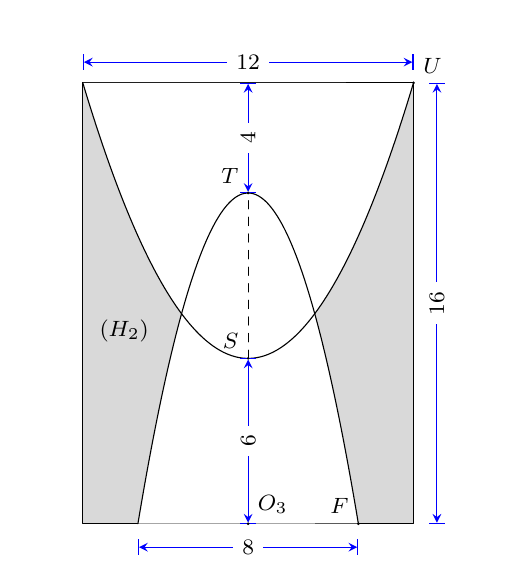
\begin{tikzpicture}[scale=.35, font=\footnotesize, line join=round, line cap=round, >=stealth]			
				\def\xmin{-8}\def\xmax{9.5}\def\ymin{-1.25}\def\ymax{18}
				\clip (\xmin,\ymin) rectangle (8.5,\ymax);					
				\draw[fill=gray!30] (-6,0)rectangle (6,16);				
				\fill[smooth,samples=200,domain=-4:4, white] plot (\x,{-.75*((\x)^2)+0*\x+12});	
				\fill[smooth,samples=200,domain=-6:6,white] plot (\x,{5/18*((\x)^2)+0*\x+6});	
				\draw[smooth,samples=200,domain=-4:4] plot (\x,{-.75*((\x)^2)+0*\x+12});	
				\draw[smooth,samples=200,domain=-6:6] plot (\x,{5/18*((\x)^2)+0*\x+6});		
				\draw[|<->|,blue] (-6,16.75)--node[black,midway,sloped,fill=white]{$12$}(6,16.75);
				\draw[|<->|,blue] (6.85,0)--node[black,midway,sloped,fill=white]{$16$}(6.85,16);	
				\draw[|<->|,blue] (-4,-.85)--node[black,midway,sloped,fill=white]{$8$}(4,-.85);				
				\draw[|<->|,blue] (0,0)--node[black,midway,sloped,fill=white]{$6$}(0,6);
				\draw[|<->|,blue] (0,12)--node[black,midway,sloped,fill=white]{$4$}(0,16);				
				\draw[dashed] (0,6)--(0,12);
				\draw (-4.5,7) node[]{$(H_2)$};
				
				\fill (4,0) node[above left]{$F$} circle (1.5pt)
				(0,12) node[above left]{$T$} circle (1.5pt)
				(0,6) node[above left]{$S$} circle (1.5pt)
				(6,16) node[above right]{$U$} circle (1.5pt)
				(0,0) node[above right]{$O_3$} circle (1.5pt)
				;
			\end{tikzpicture}
		\end{center}
		Chọn hệ trục tọa độ $Oxy$ sao cho gốc tọa độ trùng với $O_3$, tia $Ox$ và $Oy$ lần lượt trùng với tia $O_3F$ và $O_3T$ như hình vẽ.\\
		Khi đó parabol có đỉnh là $T(0,12)$ và đi qua điểm $F(4,0)$ có phương trình $$y=-\dfrac{3}{4}x^2+12.$$
		Khi đó diện tích giới hạn giữa $y=-\dfrac{3}{4}x^2+12$ là trục hoành là 
		$$S_4=2\displaystyle\int\limits_0^4\left(-\dfrac{3}{4}x^2+12\right)\mathrm{\,d}x=2\cdot 32=64.$$		
		Parabol có đỉnh $S(0,6)$ và đi qua điểm $U(6,16)$ có phương trình là $y=\dfrac{5}{18}x^2+6$.\\
		Diện tích giới hạn giữa $y=\dfrac{5}{18}x^2+6$ và đường thẳng $y=16$ là 		
		$$S_5=2\displaystyle\int\limits_0^{6}\left[16-\left(\dfrac{5}{18}x^2+6\right)\right]\mathrm{\,d}x =2\cdot 40=80.$$	
		Phương trình hoành độ giao điểm của $y=-\dfrac{3}{4}x^2+12$ và  $y=\dfrac{5}{18}x^2+6$ là
		$$\dfrac{5}{18}x^2+6= -\dfrac{3}{4}x^2+12\Leftrightarrow \dfrac{37}{36}x^2=6\Leftrightarrow \hoac{&x_1=-\dfrac{6\sqrt{222}}{37}\\&x_2=\dfrac{6\sqrt{222}}{37}.}$$
		Ta có diện tích giới hạn của $y=-\dfrac{3}{4}x^2+12$ và  $y=\dfrac{5}{18}x^2+6$ là		
		$$S_6=2\displaystyle\int\limits_0^{x_2}\left(-\dfrac{3}{4}x^2+12-\dfrac{5}{18}x^2-6\right)\mathrm{\,d}x=2\cdot\displaystyle\int\limits_0^{x_2}\left(-\dfrac{37}{36}x^2+6\right)\mathrm{\,d}x \approx 19{,}33.$$
		 Khi đó diện tích hình $(H_2)$ là $16\cdot 12- S_4-S_5+S_6\approx 67{,}33$.
	\end{itemize}
	}
\end{bt}

\begin{bt}%[2D4V3-2]
% nguon: Archive/2024/TaiLieuGiangDay/5.HH Oxyz/VDC_TDM.tex #3158

Hình phẳng $(H)$ tô màu bên dưới được tạo ra bởi một hình vuông $ABCD$ (có cạnh bằng $20$ cm và có tâm $O$) và một đường cong kín $(L)$ bao quanh hình vuông $ABCD$. Các điểm trên đường cong kín $(L)$ được tạo ra bằng cách cho một điểm $M$ chạy trên các cạnh của hình vuông $ABCD$, với mỗi điểm $M$ ta lấy trên tia đối của tia $MO$ một điểm $N$ sao cho $MN=8$ cm. Hãy tính diện tích hình phẳng $(H)$.
\begin{center}
	\begin{tikzpicture}[declare function={a=5;},scale=0.6]
		% Các điểm
		\path
		(0,0) coordinate (A)
		(a,0) coordinate (B)
		(0,-a) coordinate (D)
		($(B)+(D)$) coordinate (C)
		($(A)!0.5!(C)$) coordinate (O)
		(-2,2) coordinate (A')
		(a+2,2) coordinate (B')
		(-2,-a-2) coordinate (D')
		($(B')+(D')-(A')$) coordinate (C');
		\begin{scope}
			\path[fill=cyan!30, even odd rule]
			(A') to[bend left=30] (B') 
			to[bend left=30] (C') 
			to[bend left=30] (D') 
			to[bend left=30] (A') -- cycle
			(A)--(B)--(C)--(D)--cycle;
		\end{scope}
		\path (D)--(C)--([turn]-90:0.5) coordinate (xt)
		($(D)-(C)+(xt)$) coordinate (yt);
		\draw[dash pattern=on 2pt off 2pt] (D)--(yt) (C)--(xt);
		\draw[>=stealth,|<->|] (xt)--(yt) node[fill=white,inner sep=0pt,font=\scriptsize,pos=0.3,sloped]{$20$};
		\fill[brown!30] (A)--(B)--(C)--(D)--cycle;
		\draw[dashed,red] (A')--(B')--(C')--(D')--cycle;
		\draw (A)--(B)--(C)--(D)--cycle;
		\draw[thick] (A') to[bend left=30] (B');
		\draw[thick] (B') to[bend left=30] (C');
		\draw[thick] (C') to[bend left=30] (D');
		\draw[thick] (D') to[bend left=30] (A');
		\path ($(B)!.3!(C)$) coordinate (M);
		\path[name path=curveBC] (B') to[bend left=30] (C');
		\path[name path=rayOM] (O) -- ($(O)!3!(M)$);
		\path[name intersections={of=curveBC and rayOM, by=N}];
		\draw[dashed] 		(-4,-2.5)--(9,-2.5) (2.5,-9)--(2.5,4);
		\draw (O) -- ($(O)!1.3!(M)$);
		\draw (M) -- (N)node[above,pos=0.5]{$8$}	
		;
		\foreach \t/\g in {A/135,B/45,C/-45,D/225,O/220,M/-30,N/0} {
			\fill (\t) circle (1pt) node[shift={(\g:7pt)},font=\scriptsize] {$\t$};
		}
	\end{tikzpicture}
\end{center}
\loigiai{
	\begin{center}
		\begin{tikzpicture}[declare function={a=5;},scale=0.6]
			\path
			(0,0) coordinate (A)
			(a,0) coordinate (B)
			(0,-a) coordinate (D)
			($(B)+(D)$) coordinate (C)
			($(A)!0.5!(C)$) coordinate (O)
			(-2,2) coordinate (A')
			(a+2,2) coordinate (B')
			(-2,-a-2) coordinate (D')
			($(B')+(D')-(A')$) coordinate (C');
			\begin{scope}
				\path[fill=cyan!30, even odd rule]
				(A') to[bend left=30] (B') 
				to[bend left=30] (C') 
				to[bend left=30] (D') 
				to[bend left=30] (A') -- cycle
				(A)--(B)--(C)--(D)--cycle;
			\end{scope}
			\path (D)--(C)--([turn]-90:0.5) coordinate (xt)
			($(D)-(C)+(xt)$) coordinate (yt);
			\draw[dash pattern=on 2pt off 2pt] (D)--(yt) (C)--(xt);
			\draw[>=stealth,|<->|] (xt)--(yt) node[fill=white,inner sep=0pt,font=\scriptsize,pos=0.3,sloped]{$20$};
			\fill[brown!30] (A)--(B)--(C)--(D)--cycle;
			\draw[dashed,red] (A')--(B')--(C')--(D')--cycle;
			\draw (A)--(B)--(C)--(D)--cycle;
			\draw[thick] (A') to[bend left=30] (B');
			\draw[thick] (B') to[bend left=30] (C');
			\draw[thick] (C') to[bend left=30] (D');
			\draw[thick] (D') to[bend left=30] (A');
			\path ($(B)!.3!(C)$) coordinate (M)
			(5,-2.5)coordinate (H)node[below left]{$H$}
			(7,-2.5) node[below left]{$K$}
			(8.6,-2.5) node[below]{$E$}
			;
			\path pic["\scriptsize$\alpha$", angle eccentricity=2,draw,angle radius=12pt]{angle= H--O--M};
			\path[name path=curveBC] (B') to[bend left=30] (C');
			\path[name path=rayOM] (O) -- ($(O)!3!(M)$);
			\path[name intersections={of=curveBC and rayOM, by=N}];
			\draw[->] (-4,-2.5)--(10,-2.5)node[below]{$x$};
			\draw[->]  (2.5,-9)--(2.5,4) node[left]{$y$};
			\draw (O) -- ($(O)!1.3!(M)$) (O)--(B');
			\draw (M) -- (N)node[above,pos=0.5]{$8$}	
			;
			\foreach \t/\g in {A/135,B/120,C/-45,D/225,O/220,M/-30,N/0,B'/90} {
				\fill (\t) circle (1pt) node[shift={(\g:7pt)},font=\scriptsize] {$\t$};
			}
		\end{tikzpicture}
	\end{center}
	Ta có $OB=10\sqrt{2}$, $OH=10$, $OB'=OB+BB'=10\sqrt{2}+8$,
	 $OE=OH+HE=10+8=18=x_E$.\\
	 $\widehat{B'OK}=45^{\circ} \Rightarrow B'K=OB'\cdot \sin 45^{\circ}=\left(10\sqrt{2}+8\right)\dfrac{\sqrt{2}}{2}=10+\dfrac{5\sqrt{2}}{2}$,\\
	  $OK=OB'\cdot \cos 45^{\circ}=\left(10\sqrt{2}+8\right)\dfrac{\sqrt{2}}{2}=10+\dfrac{5\sqrt{2}}{2}=x_K$, $HK=OK-OH=10+\dfrac{5\sqrt{2}}{2}-10=\dfrac{5\sqrt{2}}{2}$.\\
	 Đặt $\widehat{MOH}=\alpha$ và gọi $S_1$ là diện tích phần giới hạn bởi $BH$, $HE$, cung $EB'$ và $BB'$.\\
	  Khi đó
	 $ON=OM+MN=\dfrac{OH}{\cos \alpha}+8=\dfrac{10}{\cos \alpha}+8$.\\
	 $\Rightarrow y_N=ON\cdot \sin \alpha=10 \tan \alpha+8\sin \alpha=10 \cdot \dfrac{y_N}{x_N}+8\cdot \dfrac{y_N}{\sqrt{x_N^2+y_N^2}}$.\\
	 $\Rightarrow 1=10 \cdot \dfrac{1}{x_N}+8\cdot \dfrac{1}{\sqrt{x_N^2+y_N^2}} \Rightarrow y_N=\sqrt{\dfrac{64}{\left(1-\dfrac{10}{x_N}\right)^2}-x_N^2}$.\\
	 Ta có 
	 $S_{\text {BHKB'}}=\dfrac{1}{2}(BH+B'K) \cdot HK=\dfrac{1}{2}\left(10+10+\dfrac{5\sqrt{2}}{2}\right) \cdot \dfrac{5\sqrt{2}}{2}=\dfrac{25+100\sqrt{2}}{4} $ (cm$^2$).\\
	 Suy ra $S_1=S_{BHKB'}+\displaystyle\int\limits_{x_K}^{x_E} \sqrt{\dfrac{64}{\left(1-\dfrac{10}{x}\right)^2}-x^2}\mathrm{\,d}x \approx 109{,}3$ (cm$^2$).\\
	 Vậy $S=8\cdot S_1 \approx 874{,}6$ (cm$^2$).
}
\end{bt}

\begin{bt}%[2D4C3-2]
% nguon: Archive/2024/TaiLieuGiangDay/5.HH Oxyz/VDC_TDM.tex #3159
%Câu 1
 Trong mặt phẳng $(\alpha)$ cho hai điểm $A, B$ cách nhau một đoạn bằng $120$, gọi $I$ là trung điểm của cạnh $AB$. Cho hình phẳng $(H)=\{M \in(\alpha) \mid MA+MI \leq 80, MI \geq 30\}$. Hãy phác hoạ và tính diện tích hình phẳng $(H)$ (làm tròn kết quả đến hàng đơn vị).
 \loigiai{
\begin{center}
\begin{tikzpicture}[line join=round, line cap=round,>=stealth]
\tikzset{every node/.style={scale=0.9}}
\coordinate (O) at (0,0);
\coordinate (A) at (-3,0);
\coordinate (I) at (3,0);
\coordinate (P) at ({4/3}, {sqrt(56)/3});
\coordinate (Q) at ({4/3}, -{sqrt(56)/3});
\draw[fill=gray!40]  (O) ellipse (4 cm and 2.6 cm);
\coordinate (M) at ($(O) + (120:4 and 2.6)$);
\draw[fill=white]  (I) circle (3 cm);
\draw  (I) circle (3 cm);
\draw (A)--(M)--(I);
\draw   (O) ellipse (4 cm and 2.6 cm);
\draw[->] (-5.1,0)--(7.1,0) node[below left] {$x$};
\draw[->] (0,-4.1)--(0,4.1) node[below left] {$y$};
\draw[->] (0.3,2) -- (1,3.5) node[right] {$S_2$};
\draw[->] (-2,1) -- (-4,3) node[left] {$S_1$};
\draw (0,0) node [below left] {$O$};
\foreach \i/\g in {A/-90,I/-90,M/120,P/90,Q/-90}{\fill[black](\i) circle (1.5pt) ($(\i)+(\g:3mm)$) node[scale=1]{$\i$};}
\end{tikzpicture}
\end{center} 
Gọi $O$ là trung điểm của $AI$, 
chọn hệ trục tọa độ như hình vẽ, đơn vị trên mỗi trục bằng $10$.\\
Tập hợp các điểm $M\in (\alpha)$ thỏa mãn $MA+MI\le 8$ là các điểm nằm bên trong  Elip $(E)$ có phương trình $\dfrac{x^2}{16}+\dfrac{y^2}{7}= 1$ (kể cả biên).\\
Tập hợp các điểm $M\in (\alpha)$ thỏa mãn $MI\ge 3$ là phần nằm bên ngoài hình tròn $(C)$ có tâm $I$, bán kính $R=3$ (kể cả những điểm nằm trên đường tròn).\\
Hình phẳng $(H)$ được tô đậm trên hình vẽ.\\
Elip $(E)$ và đường tròn $(C)$ cắt nhau tại hai điểm $P\left(\dfrac{4}{3}; \dfrac{\sqrt{56}}{3}\right)$ và $Q\left(\dfrac{4}{3}; -\dfrac{\sqrt{56}}{3}\right)$.\\
Gọi $S_1$ là diện tích của nửa Elip $(E)$, suy ra $S_1=2\pi\sqrt{7}$.\\
Gọi $S_2$ là diện tích hình phẳng nằm phía trên trục hoành, giới hạn bởi Elip $(E)$, đường tròn $(C)$ và trục tung.\\
Ta có 
\begin{eqnarray*}
S_{(H)}&=&S_1+2S_2\\
&=&2\pi\sqrt{7}+2\displaystyle\int\limits_{0}^{\tfrac{4}{3}}\left(\sqrt{7\left(1-\dfrac{x^2}{16}\right)}-\sqrt{9-(x-3)^2}\right)\mathrm{\, d}x \\
&\approx& 18{,}87.
\end{eqnarray*}
 Vậy diện tích hình $H$ bằng $1\,887$ (đ.v.d.t).

 }
\end{bt}

\begin{bt}%[2D4C3-3]
% nguon: Archive/2024/TaiLieuGiangDay/5.HH Oxyz/VDC_TDM.tex #3160

	Tính thể tích khối tròn xoay thu được khi cho hình phẳng giới hạn bởi các đường $y=x^2$, $y=2x$ quay quanh đường thẳng $d\colon y=2x$ (làm tròn kết quả đến hàng phần chục).
	\begin{center}
		\begin{tikzpicture}[scale=1, font=\footnotesize,line join=round, line cap=round, >=stealth]
			\def\a{sqrt(5)}
			\def\xmin{-5} \def\xmax{5}
			\def\ymin{-2} \def\ymax{6.5}
			\draw[->] (\xmin,0) -- (\xmax,0) node[below] {$x$};
			\draw[->] (0,\ymin) -- (0,\ymax) node[left] {$y$};
			\fill (0,0) circle (1pt) node[shift=(-145:0.25)]{$O$};
			\draw[name path = curv1,samples =100] plot[domain=-2.2:2.2] (\x,{(\x)^(2)}); 
			\draw[smooth,name path = curv2,dashed,samples =100] plot[variable =\x,domain=-2.2:2.2] ({(3/5)*\x - (-4/5)*(\x)^(2)},{(-4/5)*\x + (3/5)*(\x)^(2)}); 
			\path 
			(1,1) coordinate (A)
			(-1,-2) coordinate (X)
			(4,8) coordinate (Y)
			($(X)!(A)!(Y)$) coordinate (M)
			($(A)!2!(M)$) coordinate (B)
			;
			\draw 
			(-1,-2) -- (3,6) node [below right] {$y=2x$}
			(1.5,2.25) node [right] {$y=x^2$}
			;
			\draw[dashed]
			(A) to [out = -120, in = -120] (B) to [out = 60, in = 60] (A)
			;
			\fill [opacity = 0.2]
			(0,0) -- plot[domain=0:2.1] (\x,{(\x)^(2)}) -- (2,4) -- (0,0);
			\fill (2,4) circle (1pt) node [right] {$A$};
		\end{tikzpicture}
	\end{center}
	\loigiai{
		Chọn trục $Oh$ trùng với tia $OA$ như hình vẽ.
		\begin{center}
			\begin{tikzpicture}[scale=1, font=\footnotesize,line join=round, line cap=round, >=stealth]
				\def\a{sqrt(5)}
				\def\xmin{-5} \def\xmax{5}
				\def\ymin{-2} \def\ymax{6.5}
				\draw[->] (\xmin,0) -- (\xmax,0) node[below] {$x$};
				\draw[->] (0,\ymin) -- (0,\ymax) node[left] {$y$};
				\draw[name path = curv1,samples =100] plot[domain=-2.2:2.2] (\x,{(\x)^(2)}); 
				\draw[smooth,name path = curv2,dashed,samples =100] plot[variable =\x,domain=-2.2:2.2] ({(3/5)*\x - (-4/5)*(\x)^(2)},{(-4/5)*\x + (3/5)*(\x)^(2)}); 
				\path 
				(1,1) coordinate (A)
				(2,0) coordinate (x)
				(0,0) coordinate (O)
				(-1,-2) coordinate (X)
				(4,8) coordinate (Y)
				($(X)!(A)!(Y)$) coordinate (H)
				($(A)!2!(H)$) coordinate (B)
				($(B)!2!(H)$) coordinate (M)
				;
				\draw[->] (-1,-2) -- (3,6) node [below right] {$y=2x$};
				\node[above] at (3,6) {$h$};
				\draw (1.5,2.25) node[right] {$y=x^2$};
				\fill (O) circle (1pt) node[shift=(-145:0.25)]{$O$};
				\draw[dashed]
				(A) to [out = -120, in = -120] (B) to [out = 60, in = 60] (A)
				;
				\fill [opacity = 0.2]
				(0,0) -- plot[domain=0:2.1] (\x,{(\x)^(2)}) -- (2,4) -- (0,0);
				\draw[dashed] (M)--(H);
				\pic[draw,angle eccentricity=1.8,angle radius=3mm,"$\alpha$"]{angle=x--O--H};
				\fill (2,4) circle (1pt) node [right] {$A$};
				\foreach \x/\g in {H/150,M/-30}
				\fill (\x) circle (1pt)+(\g:2mm) node{$\x$};
			\end{tikzpicture}
		\end{center}
		Phương trình hoành độ giao điểm của parabol $y=x^2$ và đường thẳng $d\colon y=2x$ là 
		\allowdisplaybreaks
		\begin{align*}
			&x^2 = 2x \\
			\Leftrightarrow& \hoac{&x=0 \\ &x=2.}
		\end{align*}
		Suy ra $A(2;4)$. Do đó $OA = \sqrt{2^2+4^2} = 2\sqrt{5}$. \\
		Gọi $H$ là điểm thuộc đoạn $OA$. Đặt $OH=h$. \\
		Gọi $\alpha$ là góc tạo bởi tia $Ox$ và tia $OA$. \\
		Ta có $\tan\alpha = 2\Leftrightarrow \dfrac{\sin\alpha}{\cos\alpha}=2\Leftrightarrow \sin\alpha = 2\cos\alpha$. \\
		Mà $\sin^2\alpha + \cos^2\alpha = 1$ nên $4\cos^2\alpha + \cos^2\alpha = 1\Rightarrow \cos\alpha = \dfrac{\sqrt{5}}{5}$ ($\alpha$ là góc nhọn). \\
		Suy ra $\sin\alpha = \dfrac{2\sqrt{5}}{5}$. \\
		Khi đó $x_H = h\cos\alpha = \dfrac{\sqrt{5}}{5}h$, $y_H = h\sin\alpha = \dfrac{2\sqrt{5}}{5}h$. Do đó $H\left(\dfrac{\sqrt{5}}{5}h;\dfrac{2\sqrt{5}}{5}h\right)$.\\
		Đường thẳng $\Delta$ qua $H$ vuông góc với $d$ có dạng $y=-\dfrac{1}{2}x+b$. \\
		Mà $H\left(\dfrac{\sqrt{5}}{5}h;\dfrac{2\sqrt{5}}{5}h\right)\in\Delta$ nên 
		$\dfrac{2\sqrt{5}}{5}h = -\dfrac{1}{2}\cdot \dfrac{\sqrt{5}}{5}h + b\Leftrightarrow b = \dfrac{\sqrt{5}}{2}h$. \\
		Suy ra $\Delta\colon y = -\dfrac{1}{2}x + \dfrac{\sqrt{5}}{2}h$. \\
		Gọi $M$ là giao điểm của $\Delta$ và parabol $y=x^2$. \\
		Phương trình hoành độ giao điểm của $\Delta$ và parabol $y=x^2$ là
		\allowdisplaybreaks
		\begin{align*}
			&x^2 = -\dfrac{1}{2}x + \dfrac{\sqrt{5}}{2}h \\
			\Leftrightarrow&2x^2 + x - \sqrt{5}h = 0 \\
			\Leftrightarrow& \hoac{&x=\dfrac{-1-\sqrt{1+8\sqrt{5}h}}{4} \\ &x = \dfrac{-1+\sqrt{1+8\sqrt{5}h}}{4}.}
		\end{align*}
		Do $x_M>0$ nên $M\left(\dfrac{-1+\sqrt{1+8\sqrt{5}h}}{4};\dfrac{1-\sqrt{1+8\sqrt{5}h}}{8}+\dfrac{\sqrt{5}}{2}h\right)$. \\
		Khi đó $MH^2 = \left(\dfrac{-1+\sqrt{1+8\sqrt{5}h}}{4}-\dfrac{\sqrt{5}}{5}h\right)^2 + \left(\dfrac{1-\sqrt{1+8\sqrt{5}h}}{8}+\dfrac{\sqrt{5}}{10}h\right)^2$. \\
		Thể tích khối tròn xoay cần tính là
		\allowdisplaybreaks
		\begin{align*}
			V &= \displaystyle \pi\int\limits_{0}^{2\sqrt{5}}MH^2\mathrm{\,d}h \\
			&= \displaystyle \pi\int\limits_{0}^{2\sqrt{5}}\left(\dfrac{-1+\sqrt{1+8\sqrt{5}h}}{4}-\dfrac{\sqrt{5}}{5}h\right)^2 + \left(\dfrac{1-\sqrt{1+8\sqrt{5}h}}{8}+\dfrac{\sqrt{5}}{10}h\right)^2\mathrm{d}h \\
			&\approx 1{,}5.
		\end{align*}
	}
\end{bt}

\begin{bt}%[2D4H3-1]
% nguon: Archive/SP_KhoLatex/ID6_old/2-GHK2-17-THPTSo3BaoThang-LaoCai-22TN-TL.tex #3590
%[GHK2 THPT Số 3 Bảo Thắng - Lào Cai, 2022]%[Phan Quốc Trí, 12EX4-2022]
	Tính diện tích $S$ của hình phẳng giới hạn bởi đồ thị hai hàm số $y=x^3 +3x+3$ và $y=x^2+5x+3$.
	\loigiai{
		Ta có 	$x^3 +3x+3 = x^2+5x+3 \Leftrightarrow x^3 -x^2 -2x =0 \Leftrightarrow \hoac{&x=-1\\&x=0\\&x=2.}$\\
		Diện tích hình phẳng
\begin{eqnarray*}
			S&=& \displaystyle \int\limits_{-1}^{2} \left| x^3 -x^2 -2x \right| \mathrm{\,d}x\\
			& =& \displaystyle \int\limits_{-1}^{0} \left| x^3 -x^2 -2x \right| \mathrm{\,d}x + \displaystyle \int\limits_{0}^{2} \left| x^3 -x^2 -2x \right| \mathrm{\,d}x  \\
			&=& \left| \displaystyle \int\limits_{-1}^{0} \left(x^3 -x^2 -2x\right) \mathrm{\,d}x \right| + \left| \displaystyle \int\limits_{0}^{2} \left(x^3 -x^2 -2x\right) \mathrm{\,d}x \right| \\
			&=& \left| \left( \dfrac{x^4}{4}-\dfrac{x^3}{3}-x^2 \right) \Big|_{-1}^{0} \right| + \left| \left( \dfrac{x^4}{4}-\dfrac{x^3}{3}-x^2 \right) \Big|_{0}^{2} \right|\\
			&=& \dfrac{37}{12}.
\end{eqnarray*}
	}
\end{bt}

\begin{bt}%[2D4V2-5]
% nguon: Archive/SP_KhoLatex/ID6_old/2-GHK2-17-THPTSo3BaoThang-LaoCai-22TN-TL.tex #3593 
% KIEM_TRA: cần xem lại đáp số/dạng
%[GHK2 THPT Số 3 Bảo Thắng - Lào Cai, 2022]%[Phan Quốc Trí, 12EX4-2022] 
	Cho hàm số $f(x)$ liên tục trên $\mathbb{R}$ thỏa mãn $f(x)= 2x^2 -3 + \displaystyle \int\limits_{0}^{1} x f \left(\sqrt{1+3x^2 }\right) \mathrm{\,d}x$. Tính $\displaystyle \int\limits_{0}^{2} f(x) \mathrm{\,d}x$.
	\loigiai{
		Đặt $a= \displaystyle \int\limits_{0}^{1} x f \left(\sqrt{1+3x^2 }\right) \mathrm{\,d}x$. Suy ra $f(x)= 2x^2 -3 + a$. \\
		Ta có $f \left(\sqrt{1+3x^2 }\right) = 2(1+3x^2)-3+a=6x^2-1+a$. Khi đó
\begin{eqnarray*}
			& &	a = \displaystyle \int\limits_{0}^{1} x \left(6x^2-1+a \right) \mathrm{\,d}x = \displaystyle \int\limits_{0}^{1} \left( 6x^3 -x+ax \right)  \mathrm{\,d}x\\
			& \Leftrightarrow &	a= \displaystyle \int\limits_{0}^{1}  6x^3  \mathrm{\,d}x -\displaystyle \int\limits_{0}^{1}  x \mathrm{\,d}x +\displaystyle \int\limits_{0}^{1}  ax  \mathrm{\,d}x\\
			& \Leftrightarrow &	a= \dfrac{3}{2} -\dfrac{1}{2} +a \cdot\dfrac{1}{2} \Leftrightarrow a = 2.
\end{eqnarray*}	
		Suy ra $f(x)= 2x^2 -3 + 2 =2x^2 -1$. Do đó
\begin{eqnarray*}
			\displaystyle \int\limits_{0}^{2} f(x) \mathrm{\,d}x = \displaystyle \int\limits_{0}^{2} \left(2x^2 -1\right) \mathrm{\,d}x = \left(\dfrac{2}{3}x^3 -x \right) \Big|_{0}^{2} = \dfrac{10}{3}.
\end{eqnarray*}
	}
\end{bt}

\begin{bt}%[2D4V2-6]
% nguon: Archive/SP_KhoLatex/ID6_old/DeThamKhao-08.tex #3622
%[Dự án ĐGNL-ĐGTD-2022 GĐ1]%[Thành Đức Trung]
Nếu lực là một giá trị biến thiên (như kéo hay nén lò xo) và được xác định bởi hàm $F(x)$ thì công sinh ra theo trục $Ox$ từ $a$ đến $b$ là $A=\displaystyle\int\limits_{a}^{b} F(x)\mathrm{\,d}x$ (đơn vị là N). Một con lắc lò xo đang ở trạng thái tự nhiên có chiều dài $1$ mét và khi bị nén bởi một lực thì nó chỉ còn $0{,}65$ mét, biết độ cứng của lò xo là $16$ N/m. Hãy tìm công sinh ra lúc này, cho biết lực $F$ dùng để kéo hay nén lò xo đi một khoảng bằng $x$ đơn vị so với trạng thái ban đầu của lò xo thì $F$ có dạng $F=kx$ với $k$ là độ cứng của lò xo.
\loigiai
{
Một con lắc lò xo đang ở trạng thái tự nhiên có chiều dài $1$ mét và khi bị nén bởi một lực thì nó chỉ còn $0{,}65$ mét thì độ dài lò xo bị nén là $1-0{,}65=0{,}35$ (m). Với độ cứng của lò xo là $k=16$ N/m khi đó công sinh ra là
$$A=\displaystyle\int\limits_{0}^{0{,}35} 16x\mathrm{\,d}x=0{,}98 \ \text{(N).}$$
}
\end{bt}

\begin{bt}%[2D4H1-5]
% nguon: Archive/SP_KhoLatex/ID6_old/2-GHK2-24-HuongHoa-QuangTri-22.tex #3648
%[Đề thi GHK2 - THPT Hướng Hóa, Quảng Trị - 2022]%[Hoàng Thanh Phương - 12-EX4]
	Tìm họ nguyên hàm của hàm số $f(x)=\sin^{2022}x\cdot\cos x$.
\loigiai{
Xét $I=\displaystyle\int \sin^{2022}x\cdot\cos x\mathrm{\,d}x$. \\
Đặt $t=\sin x$, ta có $\mathrm{\,d}t=\cos x\mathrm{\,d}x$. \\
Khi đó $I=\displaystyle\int t^{2022}\mathrm{\,d}t=\dfrac{t^{2023}}{2023}+C=\dfrac{\sin^{2023} x}{2023}+C$.
}
\end{bt}

\begin{bt}%[2D4V2-5]
% nguon: Archive/SP_KhoLatex/ID6_old/2-GHK2-24-HuongHoa-QuangTri-22.tex #3650 
% KIEM_TRA: cần xem lại đáp số/dạng
%[Đề thi GHK2 - THPT Hướng Hóa, Quảng Trị - 2022]%[Hoàng Thanh Phương - 12-EX4]
	Cho hàm số $f(x)$ liên tục trên $\mathbb{R}$ và thỏa mãn $2022f(x)+f(-x)=\mathrm{e}^x,\,\forall x\in\mathbb{R}$. Tính tích phân $I=\displaystyle\int\limits_{-1}^1 f(x)\mathrm{\,d}x$.
\loigiai{
Đặt $x=-t$, ta có $\mathrm{\,d}x=-\mathrm{\,d}t$. \\
Đổi cận \begin{tabular}{|c|c|c|}
	\hline
	$x$& $-1$&$1$ \\
	\hline
	$t$&$1$&$-1$ \\
	\hline
\end{tabular} \\
Khi đó $I=\displaystyle\int\limits_1^{-1} -f(-t)\mathrm{\,d}t=\displaystyle\int\limits_{-1}^1 f(-t)\mathrm{\,d}t=\displaystyle\int\limits_{-1}^1 f(-x)\mathrm{\,d}x$. \\
Ta có 
\begin{eqnarray*}
	& &2022f(x)+f(-x)=\mathrm{e}^x \\
	&\Rightarrow &\displaystyle\int\limits_{-1}^1 (2022f(x)+f(-x))\mathrm{\,d}x=\displaystyle\int\limits_{-1}^1 \mathrm{e}^x\mathrm{\,d}x \\
	&\Leftrightarrow & 2023I=\mathrm{e}^x\bigg\vert_{-1}^1 =\mathrm{e}-\dfrac{1}{\mathrm{e}}
\end{eqnarray*}
Vậy $I=\dfrac{\mathrm{e}^2-1}{2023\mathrm{e}}$.
}
\end{bt}

\begin{bt}%[2D4V3-2]
% nguon: Archive/SP_KhoLatex/ID6_old/2-GHK2-24-HuongHoa-QuangTri-22.tex #3651
%[Đề thi GHK2 - THPT Hướng Hóa, Quảng Trị - 2022]%[Hoàng Thanh Phương - 12-EX4]
	\immini{
Một chiếc cổng có hình dạng là một Parabol có khoảng cách giữa hai chân cổng là $AB=8$ m. Người ta treo một tấm phông hình chữ nhật có hai đỉnh $M$, $N$ nằm trên parabol và hai đỉnh $P$, $Q$ nằm trên mặt đất (như hình vẽ). Ở phần phía ngoài phông (phần không tô đen) người ta mua hoa để trang trí với chi phí mua hoa là $150\,000$ đồng/m$^2$, biết $MN=4$ m, $MQ=6$ m. Hỏi số tiền dùng để mua hoa trang trí chiếc cổng là bao nhiêu?	
}
{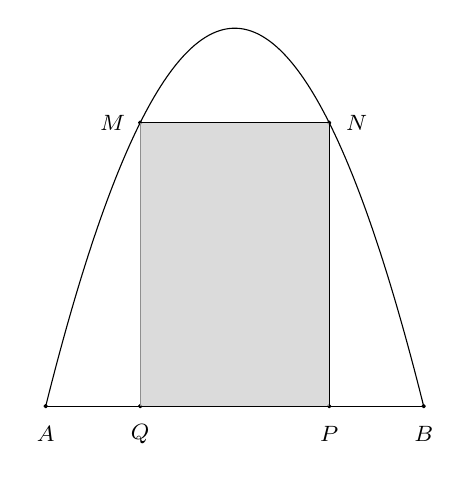
\begin{tikzpicture}[scale=0.6,>=stealth, font=\footnotesize, line join=round, line cap=round]
		\path
		(-4,0) coordinate (A)
		(-2,0)  coordinate (Q)
		(2,0) coordinate (P)
		(4,0) coordinate (B)
		(-2,6) coordinate (M)
		(2,6) coordinate (N);
\def\a{-0.5} \def\b{0} \def\c{8}
		\draw[smooth,samples=300,domain=-4:4] plot(\x,{\a*(\x)^2+\b*(\x)+\c});
		\draw (-4,0)--(4,0) (-2,0)--(-2,6)--(2,6)--(2,0);
		\foreach \x/\g in{A/-90,Q/-90,P/-90,B/-90,M/180,N/0}
		\draw[fill=black](\x)circle(1pt)node[shift={(\g:0.35)}]{$\x$};
		\fill[black!20,opacity=0.7] (Q) rectangle (N);
\end{tikzpicture}}
\loigiai{
\immini{
Chọn hệ trục tọa độ $Oxy$ như hình vẽ. \\
Parabol $(P)$ đối xứng qua $Oy$ nên phương trình parabol có dạng $y=ax^2+c$. \\
Vì parabol đi qua $B(4;0)$ và $N(2;6)$ nên $(P)\colon y=-\dfrac{1}{2}x^2+8$. \\
Diện tích hình phẳng giới hạn bởi $(P)$ và trục $Ox$ là 
$$S=2\displaystyle\int\limits_0^4 \left(-\dfrac{1}{2}x^2+8\right)\mathrm{\,d}x=\dfrac{128}{3} \,(\text{m}^2).$$  
}
{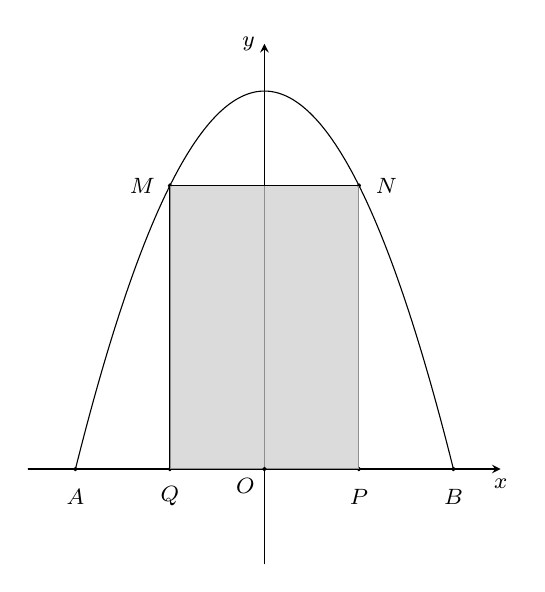
\begin{tikzpicture}[scale=0.6,>=stealth, font=\footnotesize, line join=round, line cap=round]
		\path
		(-4,0) coordinate (A)
		(-2,0)  coordinate (Q)
		(2,0) coordinate (P)
		(4,0) coordinate (B)
		(-2,6) coordinate (M)
		(2,6) coordinate (N);
		\draw[->] (-5,0)--(5,0)node[below]{$x$};
		\draw[->] (0,-2)--(0,9)node[left]{$y$};
\def\a{-0.5} \def\b{0} \def\c{8}
		\draw[smooth,samples=300,domain=-4:4] plot(\x,{\a*(\x)^2+\b*(\x)+\c});
		\draw (-2,0)--(-2,6)--(2,6)--(2,0);
		\foreach \x/\g in{A/-90,Q/-90,P/-90,B/-90,M/180,N/0}
		\draw[fill=black](\x)circle(1pt)node[shift={(\g:0.35)}]{$\x$};
		\fill[black!20,opacity=0.7] (Q) rectangle (N);
		\draw[fill=black] (0,0) circle (1pt)node[below left]{$O$};
\end{tikzpicture}}
\noindent Diện tích phần trồng hoa là 
$$S_1=S-S_{MNPQ}=\dfrac{128}{3}-24=\dfrac{56}{3} \,(\text{m}^2).$$
Vậy số tiền cần dùng để mua hoa là $\dfrac{56}{3}\cdot 150\,000=2\,8000\,000$ (đồng).
}
\end{bt}

\begin{bt}%[2D4H1-3]
% nguon: Archive/SP_KhoLatex/ID6_old/2-GHK2-25-TXQuangTri-QuangTri-22.tex #3730
%[Thi giữa học kỳ 2- THPT TX Quảng Trị- Quảng Trị - 22]%[Lê Văn Toàn - EX4]
		Biết $F(x)$ là một nguyên hàm của hàm số $f(x)=\sin 2 x$ và $F\left(\dfrac{\pi}{4}\right)=1$. Tính $F\left(\dfrac{\pi}{6}\right)$.
		\loigiai{
	Ta có $\displaystyle\int\limits_{\tfrac{\pi}{6}}^{\tfrac{\pi}{4}} \sin 2 x \mathrm{\,d} x=F\left(\dfrac{\pi}{4}\right)-F\left(\dfrac{\pi}{6}\right)=1-F\left(\dfrac{\pi}{6}\right)$.\\
	Mà $\displaystyle\int\limits_{\tfrac{\pi}{6}}^{\tfrac{\pi}{4}} \sin 2 x \mathrm{\,d} x=-\dfrac{1}{2} \cos 2 x\Big|_{\tfrac{\pi}{6}} ^{\tfrac{\pi}{4}}=-\dfrac{1}{2}\left(\cos \dfrac{\pi}{2}-\cos \dfrac{\pi}{3}\right)=\dfrac{1}{4}$.\\
	Do đó $F\left(\dfrac{\pi}{6}\right)=1-\dfrac{1}{4}=\dfrac{3}{4}$.
	}
	\end{bt}

\begin{bt}%[2D4V2-2]
% nguon: Archive/SP_KhoLatex/ID6_old/2-GHK2-25-TXQuangTri-QuangTri-22.tex #3731
%[Thi giữa học kỳ 2- THPT TX Quảng Trị- Quảng Trị - 22]%[Lê Văn Toàn - EX4]
	Cho hàm số $f(x)$ liên tục trên $\mathbb{R}$ thỏa $\displaystyle\int\limits_{0}^{1} f(x) \mathrm{\,d}x=2$ và $\displaystyle\int\limits_{0}^{2} f(3x+1) \mathrm{\,d}x=6$. Tính $I=\displaystyle\int\limits_{0}^{7} f(x) \mathrm{\,d} x$.
	\loigiai{
Ta có $A=\displaystyle\int\limits_{0}^{1} f(x) \mathrm{\,d}x=2, B=\displaystyle\int\limits_{0}^{2} f(3x+1) \mathrm{\,d}x=6$. Đặt $t=3x+1 \Rightarrow \mathrm{d}t=3 \mathrm{\,d} x$.\\
Đổi cận $x=0 \Rightarrow t=1$; $x=2 \Rightarrow t=7$.\\
Khi đó, $B=\dfrac{1}{3} \displaystyle\int\limits_{1}^{7} f(t) \mathrm{\,d}t=6 \Rightarrow \displaystyle\int\limits_{1}^{7} f(t) \mathrm{\,d}t=18 \Rightarrow \displaystyle\int\limits_{1}^{7} f(x) \mathrm{\,d}x=18$.\\
Vậy $I=\displaystyle\int\limits_{0}^{7} f(x) \mathrm{\,d}x=\displaystyle\int\limits_{0}^{1} f(x) \mathrm{\,d}x+\displaystyle\int\limits_{1}^{7} f(x) \mathrm{\,d}x=20$.
}
	\end{bt}

\begin{bt}%[2D4V3-1]
% nguon: Archive/SP_KhoLatex/ID6_old/2-GHK2-25-TXQuangTri-QuangTri-22.tex #3732
%[Thi giữa học kỳ 2- THPT TX Quảng Trị- Quảng Trị - 22]%[Lê Văn Toàn - EX4]
		\immini{
		Cho hàm số $y=f(x)$ liên tục trên $\mathbb{R}$ và hàm số $y=g(x)=x\cdot f\left(x^2\right)$ có đồ thị trên đoạn $[0;2]$ như hình vẽ.
		Biết diện tích miền tô màu là $S=\dfrac{5}{2}$, tính tích phân $I=\displaystyle\int\limits_{1}^{4} f(x) \mathrm{\,d}x$.
		}
	{
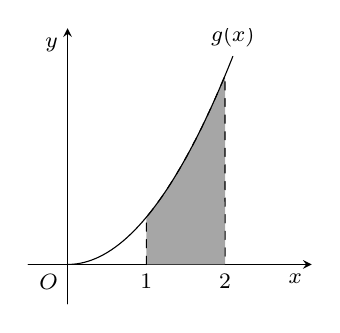
\begin{tikzpicture}[scale=1, font=\footnotesize, line join=round, line cap=round, >=stealth]
	\draw[->] (-0.5,0)--(3.1,0) node[below left] {$x$};
	\draw[->] (0,-0.5)--(0,3) node[below left] {$y$};
	\draw (0,0) node [below left] {$O$};
\begin{scope}
		\clip (-0.5,-0.5) rectangle (3,3);
		\draw[dashed,thin,fill=black!35](1,0) node[below] {$1$}--plot[samples=200,domain=1:2,smooth,variable=\x] (\x,{0.6*(\x)^2})--(2,0) node[below] {$2$};
		\draw plot[samples=200,domain=0:2.1,smooth,variable=\x] (\x,{0.6*(\x)^2}) node[above]{$g(x)$};
	\end{scope}
\end{tikzpicture}
}
\loigiai{
Ta có $S=\displaystyle\int\limits_{1}^{2} g(x) \mathrm{\,d} x=\dfrac{5}{2}=\displaystyle\int\limits_{1}^{2} x f\left(x^2\right) \mathrm{\,d} x$. Đặt $t=x^2 \Rightarrow \mathrm{\,d} t=2x \mathrm{\,d}x$.\\
Đổi cận $x=1 \Rightarrow t=1$; $x=2 \Rightarrow t=4$.\\
Khi đó, $S=\displaystyle\int\limits_{1}^{2} x f\left(x^{2}\right) \mathrm{\,d} x=\dfrac{1}{2} \displaystyle\int\limits_{1}^{4} f(t) \mathrm{\,d} t=\dfrac{5}{2} \Rightarrow \displaystyle\int\limits_{1}^{4} f(t) \mathrm{\,d} t=5 \Rightarrow \displaystyle\int\limits_{1}^{4} f(x) \mathrm{\,d} x=5$.

}
	\end{bt}

\begin{bt}%[2D4H2-3]
% nguon: Archive/SP_KhoLatex/ID6_old/2-GHK2-19-THPTTanBinh-HCM-22.tex #3752 
% KIEM_TRA: cần xem lại đáp số/dạng
%[2-GHK2-19-THPTTanBinh-HCM-22]%[Lương Như Quỳnh, 12-EX4-2022] 
	Tính $ \displaystyle \int \limits_0^{\frac{\pi}{2}} x\sin x\mathrm{\,d}x$.
	\loigiai{
	Ta có 
 $\displaystyle \int \limits_0^{\frac{\pi}{2}} x\sin x\mathrm{\,d}x 
 = - \displaystyle \int \limits_0^{\frac{\pi}{2}} x\mathrm{\,d}(\cos x)
 = (-x\cos x)\bigg|_0^{\frac{\pi}{2}}+\displaystyle \int \limits_0^{\frac{\pi}{2}} \cos x\mathrm{\,d}x
 =  (-x\cos x+\sin x)\bigg|_0^{\frac{\pi}{2}}
 = 1.$
	}	
\end{bt}

\begin{bt}%[2D4V2-5]
% nguon: Archive/SP_KhoLatex/ID6_old/2-GHK2-19-THPTTanBinh-HCM-22.tex #3754 
% KIEM_TRA: cần xem lại đáp số/dạng
%[2-GHK2-19-THPTTanBinh-HCM-22]%[Lương Như Quỳnh, 12-EX4-2022]
	Cho hàm số $ y=f(x) $ có đạo hàm liên tục trên đoạn $ [0;3] $ thỏa mãn $ \displaystyle \int \limits_0^3 f(x)\mathrm{\,d}x=10$ và $ f(3)=3 $. Tính $ \displaystyle \int \limits_0^9 f'\left(\sqrt{x}\right)\mathrm{\,d}x$.
	\loigiai{
	Xét  $ I=\displaystyle \int \limits_0^9 f'\left(\sqrt{x}\right)\mathrm{\,d}x$.\\
	Đặt $ t=\sqrt{x} \Rightarrow \mathrm{d}t=\dfrac{1}{2\sqrt{x}}\mathrm{\,d}x\Rightarrow \mathrm{d}x=2t\mathrm{\,d}t$.\\
	Đổi cận: $ \heva{&x=0\Rightarrow t=0\\&x=9\Rightarrow t=3.} $\\
	Ta có $ I= 2\displaystyle \int \limits_0^3 f'(t)t\mathrm{\,d}t=2\displaystyle \int \limits_0^3 t\mathrm{\,d}(f(t))=2tf(t)\bigg|_0^3-2\displaystyle \int \limits_0^3 f(t)\mathrm{\,d}t=6f(3)-2\cdot 10=-2$.
	}	
\end{bt}

\begin{bt}%[2D4V3-5]
% nguon: Archive/SP-4Phan-Dot3/Data/CD_2-OTHK2-De05.tex #4377
%[Dự án Đề thi 4 phần-Đợt 3]%[Đắc Vũ]
	Tại một nhà máy, gọi $C(x)$ là tổng chi phí (tính theo triệu đồng) để sản xuất $x$ tấn sản phẩm $\mathrm{A}$ trong một tháng. Khi đó, đạo hàm $\mathrm{C}'(x)$, gọi là chi phí cận biên, cho biết tốc độ tăng tổng chi phí theo lượng sản phẩm được sản xuất. Giả sử chi phí cận biên (tính theo triệu đồng trên tấn) của nhà máy được ước lượng bởi công thức
	$$
	\mathrm{C}'(x)=5-0{,}06 x+0{,}00072 x^2 \text{ với } 0 \leq x \leq 150.
	$$
	Biết rằng $\mathrm{C}(0)=30$ triệu đồng, gọi là chi phí cố định. Tính tổng chi phí (đơn vị triệu đồng) khi nhà máy sản xuất $100$ tấn sản phẩm A trong tháng.
	\loigiai{
		Ta có:
		$$
		\begin{aligned}
			\mathrm{C}(100)-\mathrm{C}(0) &=\displaystyle\int\limits_0^{100} \mathrm{C}'(x) \mathrm{\,d} x=\displaystyle\int\limits_0^{100}\left(5-0{,}06 x+0{,}00072 x^2\right) \mathrm{\,d} x \\
			&=5 \displaystyle\int\limits_0^{100} \mathrm{\,d} x-0{,}06 \displaystyle\int\limits_0^{100} x \mathrm{\,d} x+0{,}00072 \displaystyle\int\limits_0^{100} x^2 \mathrm{\,d} x \\
			&=5 x\bigg|_0 ^{100}-0{,}03 x^2\bigg|_0 ^{100}+0{,}00024 x^3\bigg|_0 ^{100}=440.
		\end{aligned}
		$$
		Suy ra $	\mathrm{C}(100)=	\mathrm{C}(0)+440=30+440=470$ (triệu đồng).\\
		Vậy khi nhà máy sản xuất $100$ tấn sản phẩm $A$ trong tháng thì tổng chi phí là $470$ triệu đồng.
	}
\end{bt}

\begin{bt}%[2D4V1-2]
% nguon: Archive/SP-4Phan-Dot3/Data/KNTT_2-OTGK2_De04.tex #4386

	Cho hàm số $y=F(x)$ là một nguyên hàm của hàm số $f(x) = 3x^2-1$ và $F(1) = 1$. Tính $F(2)$.
	\loigiai
	{
		Ta có $F(x) = \displaystyle \int  \left(3x^2-1\right) \mathrm{d}x = x^3 - x + C$.\\
		Mà $F(1) = 1 \Rightarrow C = 1$.\\
		$\Rightarrow F(x) = x^3 - x + 1$.\\
		$\Rightarrow F(2) = 7$.
	}
\end{bt}

\begin{bt}%[2D4N2-1]
% nguon: Archive/SP-4Phan-Dot3/Data/KNTT_2-OTGK2_De04.tex #4387

	Tính tích phân $\displaystyle\int\limits_{0}^{1} \left(3x^2 + 1\right) \mathrm{d}x$.
	\loigiai{
		Ta có $\displaystyle\int\limits_{0}^{1} \left(3x^2 + 1\right) \mathrm{d}x=(x^3+x)\Big|_0^1=2$.
	}	
\end{bt}

\begin{bt}%[2D4H3-1]
% nguon: Archive/SP-4Phan-Dot3/Data/KNTT_2-OTGK2_De04.tex #4388

	Tính diện tích của hình phẳng giới hạn bởi đồ thị hàm số $y=-x^2+4$ và $Ox$. 
	\loigiai{
		Phương trình hoành độ giao điểm của đồ thị hàm số $y=-x^2+4$ và $Ox$ là 
		$$-x^2+4=0\Leftrightarrow \hoac{&x=-2\\&x=2.}$$
		Diện tích hình phẳng $S = \displaystyle \int\limits_{-2}^{2} \left(-x^2+4\right) \mathrm{d}x = \dfrac{32}{3}$.
	}	
\end{bt}

\begin{bt}%[2D4V3-5]
% nguon: Archive/SP-4Phan-Dot3/Data/KNTT_2-OTGK2_De04.tex #4389

	\immini{
		Một chiếc chuông được đặt nằm ngang và gắn vào hệ tọa độ như hình vẽ. Vành của chuông là một đường cong parabol có dạng $y^2=2px$. Thể tích cái chuông là bao nhiêu (làm tròn kết quả đến hàng phần chục)?
	}{
		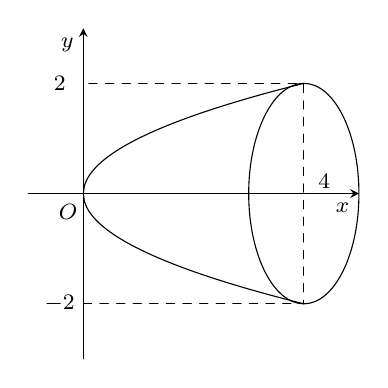
\begin{tikzpicture}[scale=0.7, font=\footnotesize, line join=round, line cap=round, >=stealth]
			
			\draw[->] (-1,0)--(5,0) node[below left] {$x$};
			\draw[->] (0,-3)--(0,3) node[below left] {$y$};
			\draw (0,0) node [shift={(-130:3mm)}] {$O$};
			\draw plot[smooth, samples=200, domain=0:4] (\x,{sqrt(\x)});
			\draw plot[smooth, samples=200, domain=0:4] (\x,-{sqrt(\x)});
			\draw[dashed]
			(0,-2)node[shift={(180:3mm)}]{$-2$}--
			(4,-2)--
			(4,0)node[shift={(30:3mm)}]{$4$}--
			(4,2)--
			(0,2)node[shift={(180:3mm)}]{$2$};
			\draw (4,0) ellipse (1 and 2);
		\end{tikzpicture}
	}
	\loigiai
	{
		Parabol đi qua điểm $(4;2)$ suy ra $p=1$.\\
		Suy ra parabol có phương trình là $y^2=x$.\\
		Thể tích của cái chuông là xoay đường cong $y=\sqrt{x}$ quanh trục hoành $Ox$ và bị giới hạn vởi hai mặt phẳng $x=0$ và $x=4$.\\
		$\Rightarrow V = \pi \displaystyle \int\limits_{0}^{4} \left(\sqrt{x}\right)^2 \mathrm{d}x = \pi \displaystyle \int\limits_{0}^{4} x \mathrm{d}x = 8\pi \approx 25{,}1$ (đvtt).
	}
\end{bt}

\begin{bt}%[2D4H1-2]
% nguon: Archive/SP-4Phan-Dot3/Data/KNTT_2-OTGK2_De03.tex #4397

	Cho $f(x)=1+|x|$. Gọi $F(x)$ là một nguyên hàm của $f(x)$ trên $\mathbb{R}$ và thỏa $F(1)=F(-1)=1$. Tính $F(-24)+F(25)$.
	\loigiai{
		Ta có $f(x)=1+|x|=\heva{&1+x \text{ khi } x \geq 0\\& 1-x \text{ khi } x < 0. }$\\
		Suy ra $F(x)=\heva{&x+\dfrac{x^2}{2}+C_1 & \text{ khi } x \geq 0\\ &x-\dfrac{x^2}{2}+C_2 & \text{ khi } x < 0.}$\\
		Theo đề $F(1)=1 \Rightarrow \dfrac{3}{2}+C_1=1 \Rightarrow C_1=\dfrac{1}{2}$.\\
		Và $F(-1)=1 \Rightarrow -\dfrac{3}{2}+C_2=1 \Rightarrow C_2=\dfrac{5}{2}$.\\
		Suy ra $F(x)=\heva{&x+\dfrac{x^2}{2}-\dfrac{1}{2} & \text{ khi } x \geq 0\\ &x-\dfrac{x^2}{2}+\dfrac{5}{2} & \text{ khi } x < 0.}$\\
		Vậy $F(-24)+F(25)=-\dfrac{619}{2}+337=\dfrac{55}{2}$.
	}
\end{bt}

\begin{bt}%[2D4N2-6]
% nguon: Archive/SP-4Phan-Dot3/Data/KNTT_2-OTGK2_De03.tex #4398

	Một vật chuyển động với vận tốc $v(t)=2t+25$ (m/s). Tìm quãng đường vật đó đi được trong $4$ giây.
	\loigiai{
	Quãng đường vật đi được trong $4$ giây là $$s=\displaystyle\int\limits_0^4\left(v(t)\right)\mathrm{\,d}t=\displaystyle\int\limits_0^4\left(2t+25\right)\mathrm{\,d}t=\left(t^2+25t\right) \Big|_0^4=116 \text{ (m) }.$$
	Vậy vật đó đi được $116$ m trong $4$ giây.
	}
\end{bt}

\begin{bt}%[2D4V3-2]
% nguon: Archive/SP-4Phan-Dot3/Data/KNTT_2-OTGK2_De03.tex #4399

	\immini{Một chiếc cổng có hình dạng là một Parabol có khoảng cách giữa hai chân cổng là $AB=8$ m. Người ta treo một tấm phông hình chữ nhật có hai đỉnh $M$, $N$ nằm trên Parabol và hai đỉnh $P$, $Q$ nằm trên mặt đất (như hình vẽ). Ở phần phía ngoài phông (phần không tô đen) người ta mua hoa để trang trí với chi phí $1$ m$^2$ cần số tiền mua hoa là $200\,000$ đồng, biết $MN=4$ m, $MQ=6$ m. Tính số tiền mua hoa trang trí chiếc cổng. (đơn vị: nghìn đồng, làm tròn đến hàng đơn vị).
	}{
		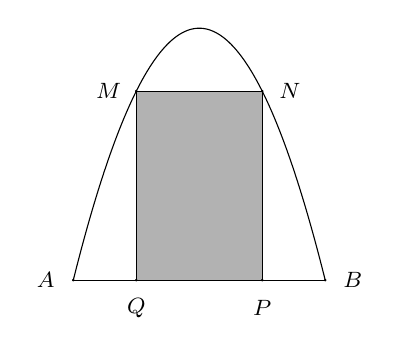
\begin{tikzpicture}[font=\footnotesize, line join=round, line cap=round, >=stealth,scale=0.4]
				\draw[samples=100,domain=-4:4]plot(\x,{-0.5*(\x)^2+8});
				\path (-2,6)coordinate(M)(2,6)coordinate(N)(-2,0)coordinate(Q)(2,0)coordinate(P)(-4,0)coordinate(A)(4,0)coordinate(B);
				\fill[gray!60,draw=black](M)--(N)--(P)--(Q)--cycle;
				\draw(A)--(B);
				\foreach \d/\g in{A/180,B/0,M/180,N/0,P/-90,Q/-90}
				\draw(\d)circle(0.7pt)node[shift={(\g:0.35)}]{$\d$};
		\end{tikzpicture}
	}
	\loigiai{
		\begin{center}
			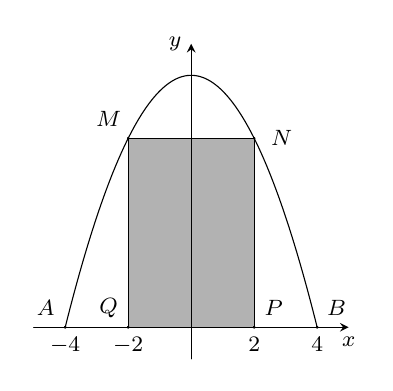
\begin{tikzpicture}[font=\footnotesize, line join=round, line cap=round, >=stealth,scale=0.4]
				\draw[samples=100,domain=-4:4]plot(\x,{-0.5*(\x)^2+8});
				\path (-2,6)coordinate(M)(2,6)coordinate(N)(-2,0)coordinate(Q)(2,0)coordinate(P)(-4,0)coordinate(A)(4,0)coordinate(B);
				\fill[gray!60,draw=black](M)--(N)--(P)--(Q)--cycle;
				\draw(A)--(B);
				\foreach \d/\g in{A/135,B/45,M/135,N/0,P/45,Q/135}
				\draw(\d)circle(0.7pt)node[shift={(\g:0.35)}]{$\d$};
				\draw [->](-5,0)--(5,0)node[below]{$x$};
				\draw [->](0,-1)--(0,9)node[left]{$y$};
				\foreach \x in{-4,-2,2,4}
				\draw(\x,0)circle(0.7pt)node[below]{$\x$};
			\end{tikzpicture}
		\end{center}
			Chọn hệ trục tọa độ như hình vẽ.\\
			Parabol đối xứng qua $Oy$ nên có dạng $(P)\colon y=ax^2+c$.\\
			Vì $(P)$ đi qua $B(4;0)$ và $N(2;6)$ nên ta có hệ $\heva{&16a+c=0\\&4a+c=6}\Leftrightarrow \heva{&a=-\dfrac{1}{2}\\&c=8.}$\\
			Suy ra $(P)\colon y=-\dfrac{1}{2}x^2+8$.\\
			Diện tích hình phẳng giới hạn bởi $(P)$ và $Ox$ là
			$$S_1=2\displaystyle\int\limits_{0}^{4} {\left(-\dfrac{1}{2}x^2+8\right)}\mathrm{\,d}x=\dfrac{128}{3} (\text{m}^2).$$
			Diện tích phần trồng hoa là $$S=S_1-S_{MNPQ}=\dfrac{128}{3}-24=\dfrac{56}{3}(\text{m}^2).$$
			Vậy số tiền dùng để mau hoa là $\dfrac{56}{3}\cdot 200\,000=3\,733\,300$ (đồng) $\approx 3\,733$ (nghìn đồng).
	}
\end{bt}

\begin{bt}%[2D4V3-2]
% nguon: Archive/SP-4Phan-Dot3/Data/KNTT_2-OTGK2_De03.tex #4400

	\immini{Một bể bơi hình elip, có độ dài trục lớn bằng $10$ m và trục nhỏ bằng $8$ m. Khu vực $A$ là chứa nước, khu vực $B$ là bậc thang lên xuống bể bơi, là nửa đường tròn có tâm là một tiêu điểm của elip, bán kính bằng $1$ m. Phần còn lại là khu vực $C$ (phần tô đậm) người ta sẽ lát gạch chống trơn. Nếu chi phí lát gạch cho mỗi mét vuông là $400$ nghìn đồng thì chi phí lát gạch cho khu vực $C$ là bao nhiêu? (đơn vị: nghìn đồng, làm tròn đến hàng đơn vị).}{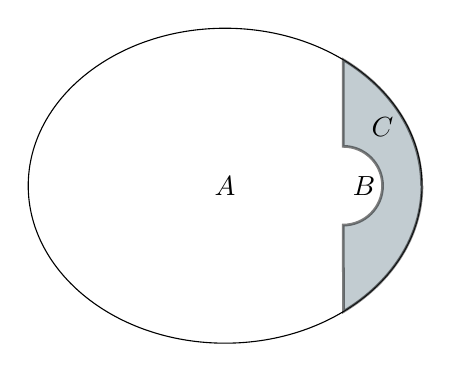
\begin{tikzpicture}[scale=0.5]
			\def\a{5}
			\def\b{4}
			\def\c{3}
			\draw (\a,0) arc(0:180:5cm and 4cm) (-\a,0) arc(180:360:5cm and 4cm);
			\coordinate (B) at (\c,0);
			\coordinate (A) at (0,0);
			\coordinate (C) at (4,1.5);
			\draw [opacity=0.5,fill=cyan!20!gray, line width=1pt](\a,0) arc(0:-53:5cm and 4cm)--(\c,-1) arc (-90:90:1cm) --(\c, 3.2) arc(53:0:5cm and 4cm);
			\path 
			node at (A){$A$}
			node at (B)[right]{$B$}
			node at (C){$C$};
	\end{tikzpicture}}
	\loigiai{
		\begin{center}
			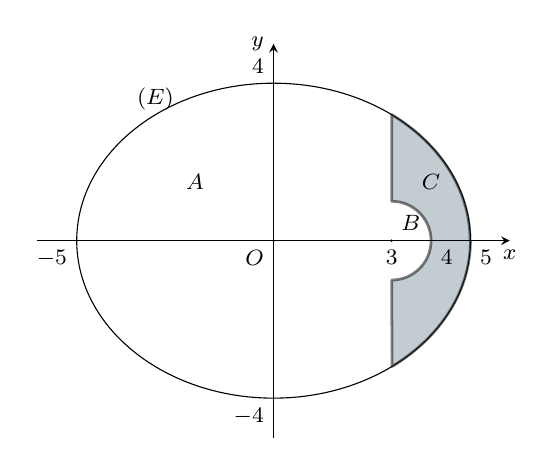
\begin{tikzpicture}[scale=0.5, font=\footnotesize, line join=round, line cap=round, >=stealth]
				\def\a{5}
				\def\b{4}
				\def\c{3}
				\draw (\a,0) arc(0:180:5cm and 4cm) (-\a,0) arc(180:360:5cm and 4cm);
				\coordinate (B) at (\c,0);
				\coordinate (A) at (0,0);
				\coordinate (C) at (4,1.5);
				\draw [opacity=0.5,fill=cyan!20!gray, line width=1pt](\a,0) arc(0:-53:5cm and 4cm)--(\c,-1) arc (-90:90:1cm) --(\c, 3.2) arc(53:0:5cm and 4cm);
				\draw[->] (-\a-1,0)--(\a+1,0)node[below]{$x$};
				\draw[->] (0,-\b-1)--(0,\b+1)node[left]{$y$};
				\path 
				node at (A)[below left]{$O$}
				node at (-2,1.5){$A$}
				node at (B)[above right]{$B$}
				node at (C){$C$}
				node at (B)[below]{$3$}
				node at (0,\b)[above left]{$4$}
				node at (\b,0)[below right]{$4$}
				node at (\a,0)[below right]{$5$}
				node at (0,-\b)[below left]{$-4$}
				node at (-\a,0) [below left]{$-5$}
				node at (-3,3.6){$(E)$};
				\foreach \x in{A,B}{
					\fill (\x) circle(1pt);
				}
			\end{tikzpicture}
		\end{center}
		Chọn hệ trục tọa độ như trên hình vẽ.\\
		Ta có phương trình chính tắc của elip $(E)\colon \dfrac{x^2}{25}+\dfrac{y^2}{16}=1$.\\
		Khi đó $y=4 \sqrt{1-\dfrac{x^2}{25}}$ là phương trình của đường elip nằm phía trên trục $Ox$.\\
		Diện tích lát gạch là 
		$$S=2\cdot \left[\displaystyle\int\limits_{3}^5 4 \sqrt{1-\dfrac{x^2}{25}}\mathrm{\,d}x - \dfrac{1}{4} \cdot \pi \cdot 1^2\right] = 8\displaystyle\int\limits_{3}^5  \sqrt{1-\dfrac{x^2}{25}}\mathrm{\,d}x - \dfrac{1}{2}\pi (\text{m}^2). $$
		Chi phí lát gạch cho khu vực $C$ là $S\cdot 400\approx 2\,950$ (nghìn đồng).
	}
\end{bt}

\begin{bt}%[2D4V3-5]
% nguon: Archive/SP-4Phan-Dot3/Data/KNTT_2-OTGK2_De02.tex #4407

	Một xe ô tô đang chuyển động đều thì người lái xe nhìn thấy chướng ngại vật trên đường. Sau $1$\,giây thì người lái xe bắt đầu đạp phanh. Kể từ lúc đạp phanh, ô tô chuyển động chậm dần đều với gia tốc $a = -5$\,m/s$^2$. Biết rằng kể từ lúc nhìn thấy chướng ngại vật đến khi dừng hẳn thì xe đi thêm được quãng đường $41{,}6$\,m. Vận tốc của xe khi người lái xe bắt đầu phanh là bao nhiêu m/s?
	\loigiai{
			Gia tốc của xe sau khi đạp phanh là $a=-5$ m/s$^2$ nên vận tốc của xe khi đó là $$v(t)=-5t+b\, (t\geq 0).$$
			Quãng đường xe đi từ lúc phanh cho đến khi dừng lại được xác định bởi công thức $$s(t)=\displaystyle\int v(t) \mathrm{\,d}t = \displaystyle\int (-5t+b) \mathrm{\,d}t = -\dfrac{5}{2}t^2+bt+c.$$
			Thời gian xe di chuyển từ lúc đạp phanh đến lúc dừng hẳn $-5t+b=0 \Leftrightarrow t=\dfrac{b}{5}$ giây.\\
			Trước khi phanh, ô tô chuyển động đều với vận tốc $v_0=v(0)=b$ m/s. Do đó trong $1$ giây xe đi được $b$ mét (điều kiện $b>0$).\\
			Quãng đường ô tô đi được từ khi bắt đầu phanh đến lúc dừng hẳn là $$s\left(\dfrac{b}{5}\right)-s(0) = -\dfrac{b^2}{10}+\dfrac{b^2}{5} = \dfrac{b^2}{10}.$$
			Theo bài ra, ta có phương trình $\dfrac{b^2}{10}+b=41{,}6 \Leftrightarrow b^2+10b-416=0 \Rightarrow b=16$.\\
			Vậy vận tốc của ô tô trước khi người lái bắt đầu phanh là $v_0=16$ m/s.
	}
\end{bt}

\begin{bt}%[2D4N2-1]
% nguon: Archive/SP-4Phan-Dot3/Data/KNTT_2-OTGK2_De02.tex #4408

	Cho hàm số $f(x)$ liên tục trên $\mathbb{R}$. Biết $\displaystyle\int \limits_0^3{f(x)\mathrm{\,d}x}=3$. Tính $\displaystyle \int \limits_0^3{2f(x)\mathrm{\,d}x}$.
	\loigiai{
		Ta có
			$\displaystyle \int \limits_0^3{2f(x)\mathrm{\,d}x}=2\displaystyle\int \limits_0^3{f(x)\mathrm{\,d}x}=2\cdot 3=6$.
	}
\end{bt}

\begin{bt}%[2D4H3-3]
% nguon: Archive/SP-4Phan-Dot3/Data/KNTT_2-OTGK2_De02.tex #4409

	Cho hình phẳng $(H)$ giới hạn bởi đồ thị hàm số $y=\dfrac{x+1}{x}$, trục hoành và hai đường thẳng $x=2$, $x=6$. Tính diện tích hình phẳng $(H)$.
	\loigiai{
		Diện tích hình phẳng $(H)$ là\\
			$$S=\displaystyle \int\limits_2^6{\left|\dfrac{x+1}{x}\right|\mathrm{d}x}=\displaystyle \int\limits_2^6{\left(1+\dfrac{1}{x}\right)\mathrm{d}x}=\left(x+\ln x\right)\Big|_2^6=4+\ln 3.$$
	}
\end{bt}

\begin{bt}%[2D4V3-3]
% nguon: Archive/SP-4Phan-Dot3/Data/KNTT_2-OTGK2_De02.tex #4410

	\immini[thm]{Một chậu nước có hình dạng như hình bên bằng mặt phẳng song song và cách mặt đáy $x$ cm $(0\le x\le 16)$ thì mặt cắt hình tròn có bán kính $\left(10+\sqrt x\right)$ cm. Tìm $x$ (đơn vị cm, làm tròn kết quả đến hàng phần trăm) để dung tích nước trong chậu bằng nửa thể tích của chậu.
	}{
		\begin{tikzpicture}[font=\footnotesize, line join=round, line cap=round,scale=.7]
			\def\l{4}
			\pgfmathsetmacro{\m}{\l*sin(45)}
			\pgfmathsetmacro{\n}{\l*sin(75)}
			\coordinate (O) at ($ (0,0) $);
			\coordinate (A) at ($(O)+ (0:\l cm )$);
			\coordinate (A') at ($(O)+(180:\l cm )$);%
			\coordinate (a) at ($(A)+ (0.5,0)$);%
			\coordinate (a') at ($(A')+ (0.5,0)$);%
			\coordinate (B) at ($(O)+ (-45:\l cm )$);
			\coordinate (B') at ($(O)+ (-135:\l cm )$);
			\coordinate (C) at ($(O)+ (-15:\l cm )$);
			\coordinate (C') at ($(O)+ (-165:\l cm )$);
			\coordinate (I) at ($(C)!1/2!(C')$);
			\coordinate (J) at ($(B)!1/2!(B')$); 
			\fill[color=cyan!20](C)arc(0:180:{\n} and {0.2*\n})--(C) arc (-15:-45:{\n})--(B)arc(0:-180:{\m} and {0.2*\m})--(B') arc (-135:-165:{\n}); 
			\draw (A) arc(0:360:{\l} and {0.2*\l});
			\draw (A)arc(0:-45:{\l});
			\draw (A') arc(-180:-135:{\l});
			\draw (B)arc(0:-180:{\m} and {0.2*\m});
			\draw[dashed] (B)arc(0:180:{\m} and {0.2*\m});
			\draw (C)arc(0:-180:{\n} and {0.2*\n});
			\draw[dashed] (C)arc(0:180:{\n} and {0.2*\n});
			\draw (1.5,-0.9) node[below]{$10+\sqrt x$};
			\draw[<->, thick](J)--(I) node[midway, right]{$x$ cm};
			\draw[<->, thick](J)--(O) node[midway, left]{$16$ cm}; 
		\end{tikzpicture}
	}
	\loigiai{
		Diện tích của mặt cắt là $S(x)=\pi\left(10+\sqrt x\right)^2 = \pi \left(100+20\sqrt{x}+x\right)$.\\
		Dung tích của chậu là
		\allowdisplaybreaks
		\begin{align*}
			V=\displaystyle\int\limits_0^{16} S(x)\mathrm{\,d}x =
			\pi \displaystyle\int\limits_{0}^{16} \left(100+20\sqrt{x}+x\right)\mathrm{d}x  = \pi \left(100x+ \dfrac{x^2}{2} + \dfrac{40}{3} x^{\tfrac{3}{2}}\right)\bigg|_0^{16} = \dfrac{7\,744}{3}\pi.
		\end{align*}
		Gọi $h$ là chiều cao của phần nước trong chậu. Lượng nước chứa trong chậu có thể tích là
		\allowdisplaybreaks
		\begin{align*}
			V_h =&\, \displaystyle\int\limits_0^h S(x)\mathrm{\,d}x =\pi \displaystyle\int\limits_0^h \left(100+20\sqrt{x}+x\right)\mathrm{d}x\\
			=&\, \pi\left(100x +\dfrac{x^2}{2} +\dfrac{40}{3}x^{\tfrac{3}{2}}\right)\bigg|_0^h=\pi\left(100h + \dfrac{h^2}{2} + \dfrac{40}{3}h\sqrt{h}\right).
		\end{align*}
		Theo bài ra ta có phương trình
		\[100h + \dfrac{h^2}{2} + \dfrac{40}{3}h\sqrt{h}=\dfrac{1}{2} \cdot\dfrac{7\,744}{3} \Leftrightarrow 3h^2+80h\sqrt{h}+600h-7\,744=0\]
		Đặt $k = \sqrt{h}>0$, do đó $h = k^2$. Phương trình trở thành $$3k^4 +80k^3+ 600k^2 - 7\,744 = 0\Rightarrow k\approx2{,}99\Rightarrow h\approx 8{,}94 \,\mathrm{cm}.$$
	}
\end{bt}

\begin{bt}%[2D4V2-6]
% nguon: Archive/SP-4Phan-Dot3/Data/CD_2-OTHK2-De01.tex #4418
%[Dự án đè thi 4 phần đợt 3]%[Trần Xuân Hòa]
	Một chất điểm $A$ xuất phát từ $O$ chuyển động thẳng với vận tốc biến thiên theo thời gian bởi quy luật $v(t)=\dfrac{1}{150}t^2+\dfrac{59}{75}t$ (m/s), trong đó $t$ (giây) là khoảng thời gian tính từ lúc $A$ bắt đầu chuyển động. Từ trạng thái nghỉ, một chất điểm $B$ cũng xuất phát từ $O$, chuyển động thẳng cùng hướng với $A$ nhưng chậm hơn $3$ giây so với $A$ và có gia tốc bằng $a$ (m/s$^2$) ($a$	là hằng số). Sau khi $B$ xuất phát được $12$ giây thì đuổi kịp $A$. Tính vận tốc của $B$ tại thời điểm đuổi kịp $A$. 
	\loigiai{
			Quãng đường chất điểm $A$ đi từ đầu đến khi $B$ đuổi kịp là \\
				 $$S_1=\displaystyle\int\limits_0^{15} \left (\dfrac{1}{150}t^2+\dfrac{59}{75}t\right ) \mathrm{\,d}t=96~(\text{m}).$$
			Vận tốc của chất điểm $B$ là $v_B(t) =\displaystyle\int a \mathrm{\,d}t=at+C$.\\
			Tại thời điểm $t=3$ vật $B$ bắt đầu từ trạng thái nghỉ nên $v_B(3)=0\Leftrightarrow C=-3a$. \\
			Lại có quãng đường chất điểm $B$ đi được đến khi gặp $A$ là  $S_2 =\displaystyle\int\limits_3^{15}  (at-3a ) \mathrm{\,d}t=72a~(\text{m})$. \\
		Vậy  $ 72a=96\Leftrightarrow a=\dfrac{4}{3}$ (m/s$^2$). \\
		Tại thời điểm đuổi kịp $A$ thì vận tốc của $B$ là $v_B(15)=16$ (m/s).
		}
\end{bt}

\begin{bt}%[2D4H1-6]
% nguon: Archive/SP-4Phan-Dot3/Data/KNTT_2-OTGK2_De01.tex #4429

	Cây cà chua khi trồng có chiều cao $5$ cm . Tốc độ tăng chiều cao của cây cà chua sau khi trồng được cho bởi hàm số $v(t)=-0{,}1t^3+t^2$, trong đó $t$ tính theo tuần, $v(t)$ tính bằng centimét/tuần. Gọi $h(t)$ (tính bằng centimét) là độ cao của cây cà chua ở tuần thứ $t$. Vào thời điểm cây cà chua đó phát triển nhanh nhất thì chiều cao cây cà chua đạt $54{,}4$ cm. (Kết quả được làm tròn đến hàng phần mười)
	\loigiai{
		Ta có $\displaystyle\int\left(-0{,}1t^3+t^2\right)\mathrm{\,d}t=\displaystyle\int  -0{,}1t^3\mathrm{~d}t+\int  t^2\mathrm{~d}t=\dfrac{-t^4}{40}+\frac{t^3}{3}+C$. \\
		Do $h(t)$ là một nguyên hàm của $v(t)$ nên $h(t)=\dfrac{-t^4}{40}+\dfrac{t^3}{3}+C$\\
		Cây cà chua khi trồng có chiều cao 5 cm nên $h(0)=5$, suy ra $C=5$.\\
		Vậy $h(t)=\dfrac{-t^4}{40}+\dfrac{t^3}{3}+5,\,\,t\geq0$.\\
		Ta cần tìm giá trị lớn nhất của hàm số $v(t)=-0{,}1t^3+t^2$ với $t\in[0;10]$. \\
		Ta có $v'(t)=-0{,}3t^2+2t=-0{,}3t\left(t-\dfrac{20}{3}\right)$, suy ra $v'(t)=0$ khi $t$ bằng 0 hoặc $\dfrac{20}{3}$. \\
		Ta thấy $v(0)=0$, $v\left(\dfrac{20}{3}\right)=\dfrac{400}{27}$, $v(10)=0$.\\
		Khi đó $v(t)$ đạt giá trị lớn nhất bằng $\dfrac{400}{27}$ trên đoạn $[0;10]$ tại $t=\dfrac{20}{3}$.\\ Ta có $h\left(\dfrac{20}{3}\right)=\dfrac{4\,405}{81}\approx54{,}4$.
	}
\end{bt}

\begin{bt}%[2D4H3-1]
% nguon: Archive/SP-4Phan-Dot3/Data/KNTT_2-OTGK2_De01.tex #4430

	Cho hình $(H)$ giới hạn bởi các đường $y=\dfrac{2}{x}$, $y=0$, $x=1$ và $x=4$. Gọi $x=k$ là đường thẳng chia hình $(H)$ thành $2$ phần có diện tích bằng nhau. Khi đó $k=1$.
	\loigiai{
		\begin{center}
			\begin{tikzpicture}[scale=1, font=\footnotesize, line join=round, line cap=round, >=stealth]
				\draw[->] (-1,0)--(4.5,0) node[below] {$x$} ;
				\draw[->] (0,-0.6)--(0,2.5) node[right] {$y$} ;
				\draw[fill=black] (0,0) node[below left] {$O$};
				\draw[domain=0.8:4.4] plot(\x,{2/(\x)}) ;
				\draw[color=black,fill=black,pattern=north east lines,pattern color=black] {[smooth,samples=100,domain=1:4] plot(\x,{2/(\x)})} -- (4, 0)-- (1,0) -- cycle;
				\draw[dashed] (2,-.61)--(2,2) node[below right] {$x=k$};
				\draw (1,0) node[below] {$1$};
				\draw(4,0) node[below]{$4$};
				\fill (1,0) circle (1pt) (0,0) circle (1pt) (4,0) circle (1pt);
			\end{tikzpicture}
		\end{center}
		Diện tích hình $(H)$ bằng $S=\displaystyle\int\limits_1^4\dfrac{2}{x}\mathrm{\,d}x=4\ln 2$.\\
		Đường thẳng $x=k$ chia hình $(H)$ thành $2$ phần có diện tích bằng nhau nên $$\displaystyle\int\limits_1^k\dfrac{2}{x}\mathrm{\,d}x=2\ln 2\Leftrightarrow\left(2\ln x\right)\bigg|_1^k=2\ln 2\Leftrightarrow 2\ln k=2\ln 2\Leftrightarrow k=2.$$
	}
\end{bt}

\begin{bt}%[2D4V1-6]
% nguon: Archive/SP-4Phan-Dot3/Data/KNTT_2-OTGK2_De01.tex #4431

	Một viên đạn được bắn thẳng đứng lên trên từ mặt đất. Giả sử tại thời điểm $t$ giây (coi $t=0$ là thời điểm viên đạn được bắn lên), vận tốc của nó được cho bởi $v(t)=25-9{,}8t\,(\mathrm{m/s})$. Độ cao của viên đạn (tính từ mặt đất) đạt giá trị lớn nhất bằng bao nhiêu? (Kết quả tính bằng đơn vị mét và làm tròn đến hàng phần chục)
	\loigiai{
		Gọi $h(t)$ là độ cao của viên đạn bắn lên từ mặt đất sau $t$ giây kể từ thời điểm đạn được bắn lên.\\
		Khi đó $h(t)=\displaystyle\int  v(t)\mathrm{\,d}t=\int  (25-9{,}8t)\mathrm{\,d}t=25t-4{,}9t^2+C$ (m).\\
		Do $h(0)=0$ nên $C=0\Rightarrow h(t)=-4{,}9t^2+25t$ (m).\\
		Vậy viên đạn đạt độ cao lớn nhất là $h=-\dfrac{\Delta}{4a}=\dfrac{3\,125}{98}\approx31{,}9$ (m) khi $t=-\dfrac{b}{2a}=\dfrac{125}{49}$ giây.}
\end{bt}

\begin{bt}%[2D4V2-6]
% nguon: Archive/SP-4Phan-Dot3/Data/KNTT_2-OTGK2_De01.tex #4432

	Gia tốc tại thời điểm $t$ của một vật chuyển động thẳng được cho bởi công thức $a(t)=4\pi\cos t\,\left(\mathrm{cm/s^2}\right)$. Nếu vận tốc của vật bằng $0$ tại thời điểm $t=0$ thì vận tốc trung bình (cm/s) của vật trong khoảng thời gian $0\leq t\leq \pi$ là bao nhiêu?
	\loigiai{
		Ta có $v(t)=\displaystyle\int  a(t)\mathrm{\,d}t=\displaystyle\int  4\pi\cos t\mathrm{~d}t=4\pi\sin t+C$.\\
		Do $v(0)=0$ suy ra $C=0$. Vậy $v(t)=4\pi\sin t$.\\
		Vận tốc trung bình của vật trong khoảng thời gian $0\leq t\leq \pi$ là		
		$$
		\frac{1}{\pi }\displaystyle\int\limits_0^\pi v(t)\mathrm{\,d}t=\dfrac{1}{\pi }\displaystyle\int\limits_0^\pi 4\pi\sin t\mathrm{~d}t=-4\cos t\bigg|_0^\pi =8\,\,(\mathrm{cm}/\mathrm{s}).
		$$
	}
\end{bt}

\begin{bt}%[2D4N2-2]
% nguon: Archive/SP-4Phan-Dot3/Data/CD_2-OTGK2-De04.tex #4440
%[Dự án đề 4 phần]%[Đoàn Hùng]
	Tính diện tích hình phẳng giới hạn bởi đồ thị hàm số $y=\ln x$, trục $Ox$ và đường thẳng $x=\mathrm{e}$.
	\loigiai{
		Ta có $\ln x=0\Leftrightarrow x=1$. Vậy $S=\displaystyle\int\limits_0^{\mathrm{e}}|\ln x|\mathrm{\,d}x=1$.}
\end{bt}

\begin{bt}%[2D4V3-1]
% nguon: Archive/SP-4Phan-Dot3/Data/CD_2-OTGK2-De04.tex #4441
%[Dự án đề 4 phần]%[Đoàn Hùng]
	Tính diện tích hình phẳng giới hạn bởi đồ thị của hai hàm số $y=x^2$, $y=2-x$ và hai đường thẳng $x=0$, $x=2$.
	\loigiai{
		\immini{
			Diện tích cần tìm là $$S=\displaystyle\int\limits_{0}^{2} |x^2-(2-x)|
			\mathrm{\,d}x=\displaystyle\int\limits_{0}^{2} |x^2+x-2|
			\mathrm{\,d}x$$
			Ta có $x^2+x-2=0\Leftrightarrow x=1$ hoặc $x=-2$.
			\begin{align*}
				\text{Vậy } S&=\displaystyle\int\limits_{0}^{1} |x^2+x-2|
				\mathrm{\,d}x+\displaystyle\int\limits_{1}^{2} |x^2+x-2|
				\mathrm{\,d}x\\
				&=\left|\displaystyle\int\limits_{0}^{1} (x^2+x-2)
				\mathrm{\,d}x\right|+\left|\displaystyle\int\limits_{1}^{2} (x^2+x-2)
				\mathrm{\,d}x\right|\\
				&=\left|\left(\dfrac{x^3}{3}+\dfrac{x^2}{2}-2x\right)\bigg|_0^1\right|+\left|\left(\dfrac{x^3}{3}+\dfrac{x^2}{2}-2x\right)\bigg|_1^2\right|\\
				&=\left|-\dfrac{7}{6}\right|+\left|\dfrac{11}{6}\right|\\
				&=3.
		\end{align*}}
		{\begin{tikzpicture}				
				\fill[fill=black,pattern=north east lines,pattern color=black](0,0)--plot[domain=0:1](\x,{\x*(\x)})--
				plot[domain=1:0](\x,{2-\x})--(0,2)--cycle;
				\fill[fill=black,pattern=north east lines,pattern color=black](1,1)--plot[domain=1:2](\x,{\x*(\x)})--(2,4)--(2,0)--
				plot[domain=2:1](\x,{2-\x})--cycle;
				\draw[dashed](1,0)--(1,1);
				\draw(2,-2)--(2,5); \path (2,2)node[right]{$x=2$}; 
				\draw[thick,samples=150,smooth,domain=-2.5:3.3] plot(\x,{2-\x})node[below ]{$y=2-x$};
				\draw[thick,samples=150,smooth,domain=-2.2:2.2]          
				plot(\x,{\x*(\x)})node[ right]{$y=x^2$};
				\foreach \d in {1,2}{\path (\d,0)node[below left]{$\d$};}
				\foreach \d in {2,4}{\path (0,\d)node[below left]{$\d$};}
				\foreach \i in{-1,1,3}{\draw(\i,-.1)--(\i, .1);}
				\foreach \i in{-1,1,2,3,4}{\draw(-.1,\i)--( .1,\i);}
				
				\path (0,0)node[below left]{$O$};
				\draw[->] (-2,0)--(4,0)node[below]{$x$};
				\draw[->] (0,-2)--(0,5)node[left]{$y$};
			\end{tikzpicture}
			%	\caption{ }
			%\end{figure}
		}
	}
\end{bt}

\begin{bt}%[2D4V3-2]
% nguon: Archive/SP-4Phan-Dot3/Data/CD_2-OTGK2-De01.tex #4453

	Trong chương trình nông thôn mới, tại một xã Y có xây một đoạn đường hầm bằng bê tông như hình vẽ. Tính thể tích khối bê tông để đổ đủ đoạn đường hầm. (Đường cong trong hình vẽ là các đường Parabol).
	\begin{center}
		\begin{tikzpicture}[scale=1, font=\footnotesize, line join=round, line cap=round, >=stealth]
			\path 
			(0,0) coordinate (O)
			(0,1) coordinate (B)
			(-1,0) coordinate (A)
			(1,0) coordinate (C)
			($(B)+(0,0.5)$) coordinate (E)
			($(A)+(-0.5,0)$) coordinate (D)
			($(C)+(0.5,0)$) coordinate (F)
			;
			\foreach \i in {O,A,B,C,D,E,F}
			\path ($(\i)+(-6,-2)$) coordinate (\i');
			\draw (E)--(E') (F)--(F')
			(D')--(F') node[midway,below]{$19$};
			\draw[dashed] %(O)--(O')
			(A)--(A') (B)--(B') (D)--(D') (C)--(C')
			(D)--(F) 
			;
			\draw[<->] ($(A')-(0,0.2)$)--($(D')-(0,0.2)$) node[midway,below]{$0{,}5$};
			\draw[<->] ($(F')-(0,0.2)$)--($(C')-(0,0.2)$) node[midway,below]{$0{,}5$};
			
			\draw[<->] ($(O)+(0.1,0)$)--($(B)+(0.1,0)$) node[midway,right]{$2$};
			\draw[<->] (B)--(E) node[midway,right]{$0{,}5$};
			\begin{scope}
				\draw[samples=350,domain=-1.5:1.5,smooth,variable=\x] plot (\x,{(-2/3)*(\x)^2+1.5});
				\draw[samples=350,domain=-1:1,smooth,variable=\x] plot (\x,{-(\x)^2+1});
				\draw[samples=350,domain=-7.5:-4.5,smooth,variable=\x] plot (\x,{(-2/3)*(\x+6)^2-0.5});
				\draw[samples=350,domain=-7:-5,smooth,variable=\x] plot (\x,{-(\x+6)^2-1});
			\end{scope}
		\end{tikzpicture}
	\end{center}
	\loigiai{
		Chọn hệ trục $Oxy$ như hình vẽ.\\
		\begin{center}
			\begin{tikzpicture}[scale=1, font=\footnotesize, line join=round, line cap=round, >=stealth]
				\draw[->] (0,0)--(1.5,0) node[below]{$x$};
				\draw[->] (0,0)--(0,2) node[left]{$y$};
				\draw[fill=black] (0,0) circle(1pt) node[below left]{$O$};
				\path 
				(0,0) coordinate (O)
				(0,1) coordinate (B)
				(-1,0) coordinate (A) node[above right]{$B$}
				(1,0) coordinate (C) node[above right]{$A$}
				($(B)+(0,0.5)$) coordinate (E)
				($(A)+(-0.5,0)$) coordinate (D)
				($(C)+(0.5,0)$) coordinate (F)
				;
				\foreach \i in {O,A,B,C,D,E,F}
				\path ($(\i)+(-6,-2)$) coordinate (\i');
				\draw (E)--(E') (F)--(F')
				(D')--(F');
				\draw[dashed] %(O)--(O')
				(A)--(A') (B)--(B') (D)--(D') (C)--(C')
				(D)--(F) 
				;
				\draw[<->] ($(A')-(0,0.2)$)--($(D')-(0,0.2)$) node[midway,below]{$0{,}5$};
				\draw[<->] ($(F')-(0,0.2)$)--($(C')-(0,0.2)$) node[midway,below]{$0{,}5$};
				%\draw[<->] ($(O)+(0.1,0)$)--($(B)+(0.1,0)$) node[midway,right]{$2$};
				%	\draw[<->] (B)--(E) node[midway,right]{$0{,}5$};
				\begin{scope}
					\draw[samples=350,domain=-1.5:1.5,smooth,variable=\x] plot (\x,{(-2/3)*(\x)^2+1.5});
					\draw[samples=350,domain=-1:1,smooth,variable=\x] plot (\x,{-(\x)^2+1});
					\draw[samples=350,domain=-7.5:-4.5,smooth,variable=\x] plot (\x,{(-2/3)*(\x+6)^2-0.5});
					\draw[samples=350,domain=-7:-5,smooth,variable=\x] plot (\x,{-(\x+6)^2-1});
				\end{scope}
			\end{tikzpicture}
		\end{center}
		Gọi $(P_1)\colon y=a_1 x^2+b_1$ là Parabol đi qua hai điểm $A\left( \dfrac{19}{2};0 \right)$, $B(0;2)$.\\
		Nên ta có hệ phương trình sau: 
		$$\heva{&0=a\left( \dfrac{19}{2} \right)^2+2\\&2=b}
		\Leftrightarrow \heva{&a_1=-\dfrac{8}{361}\\&b_1=2}
		\Rightarrow (P_1)\colon y=-\dfrac{8}{361}{x^2}+2.$$
		Gọi $(P_2)\colon y=a_2x^2+b_2$ là Parabol đi qua hai điểm $C\left( 10;0 \right)$, $D\left( 0;\dfrac{5}{2} \right)$.\\
		Nên ta có hệ phương trình sau: 
		$$\heva{&0=a_2\left( 10 \right)^2+\dfrac{5}{2}\\&\dfrac{5}{2}=b_2}
		\Leftrightarrow \heva{&a_2=-\dfrac{1}{40}\\&b_2=\dfrac{5}{2}}
		\Rightarrow (P_2)\colon y=-\dfrac{1}{40} x^2+\dfrac{5}{2}.$$
		Ta có thể tích của bê tông là 
		$$ V=5\cdot 2\left[ \int_0^{10} \left( -\dfrac{1}{40}{x^2}+\dfrac{5}{2} \right)\mathrm{\,d}x- \int_0^{\tfrac{19}{2}} \left( -\dfrac{8}{361}{x^2}+2 \right)\mathrm{\,d}x \right]
		=40~\text{m}^3.$$
	}
\end{bt}

\begin{bt}%[2D4C2-2]
% nguon: Archive/SP-4Phan-Dot3/Data/CD_2-OTGK2-De01.tex #4456

	Cho hai đường tròn $(O_1;10)$ và $(O_2;6)$ cắt nhau tại hai điểm $A$, $B$ sao cho $AB$ là một đường kính của đường tròn $(O_2;6)$. Gọi $(D)$ là hình phẳng được giới hạn bởi hai đường tròn (ở ngoài đường tròn lớn, phần được gạch chéo như hình vẽ). Quay $(D)$ quanh trục $O_1 O_2$ ta được một khối tròn xoay. Tính thể tích $V$ của khối tròn xoay được tạo thành.
\begin{center}
\begin{tikzpicture}[scale=0.75, font=\footnotesize, line join=round, line cap=round, >=stealth]
	\draw (-{sqrt(13)},0)--(5,0); % Vẽ trục hoành
	% Vẽ tâm O1 và O2
	\fill[black] (0,0) circle (1pt) node[below] {$O_1$};
	\fill[black] (3,0) circle (1pt) node[below left] {$O_2$};
	% Vẽ đường tròn c1 và c2
	\draw[name path=c1] (0,0) circle[radius=sqrt(13)];
	\draw[name path=c2] (3,0) circle (2);
	% Tìm và nối giao điểm A và B
	\path [name intersections={of=c1 and c2, by={A, B}}];
	\draw (A)--(B);
	% Vẽ các điểm A và B
	\foreach \x/\g in {A/70,B/-70}
	\fill[black] (\x) circle (1pt) ($(\g:3mm)+(\x)$) node {$\x$};
	% Vẽ điểm C
	\draw (5,0) node[right] {$C$};
	\fill[black] (5,0) circle (1pt);
	% Tô màu miền giới hạn bởi hai cung AB của O1 và O2
	\fill[opacity=.8,pattern=north west lines] 
	(B) arc ({-asin(2/sqrt(13))}:{asin(2/sqrt(13))}:{sqrt(13)}) % Cung tròn từ B đến A trên O1
	arc (90:-90:{2});  % Cung tròn từ A đến B trên O2
\end{tikzpicture}
\end{center}
	
	\loigiai
	{
		Chọn hệ tọa độ $Oxy$ với $O_2 \equiv O$, $O_2 C \equiv Ox$, $O_2 A \equiv Oy$.\\
		Cạnh $O_1 O_2=\sqrt{O_1 A^2-O_2 A^2}=\sqrt{10^2-6^2}=8 \Rightarrow(O_1)\colon (x+8)^2+y^2=100$.\\
		Phương trình đường tròn $(O_2)\colon x^2+y^2=36$.\\
		Kí hiệu $(H_1)$ là hình phẳng giới hạn bởi các đường $y=\sqrt{100-(x+8)^2}$, trục $Ox$, $x=0$, $x=2$.\\	
		Kí hiệu $(H_2)$ là hình phẳng giới hạn bởi các đường $y=\sqrt{36-x^2}$, trục $Ox$, $x=0$, $x=6$.\\
		Khi đó thể tích $V$ cần tính chính bằng thể tích $V_2$ của khối tròn xoay thu được khi quay hình $(H_2)$ xung quanh trục $Ox$ trừ đi thể tích $V_1$ của khối tròn xoay thu được khi quay hình $(H_1)$ xung quanh trục $Ox$.\\
		Ta có $V_2=\dfrac{1}{2} \cdot \dfrac{4}{3} \pi r^3=\dfrac{2}{3} \pi \cdot 6^3=144 \pi$.\\
		Lại có $V_1=\pi \displaystyle\int_0^2 y^2 \mathrm{\,d}x=\pi \displaystyle\int_0^2 [100-(x+8)^2] \mathrm{\,d}x=\dfrac{112 \pi}{3}$.\\
		Do đó $V=V_2-V_1=144 \pi-\dfrac{112 \pi}{3}=\dfrac{320 \pi}{3}$.
	}
\end{bt}

\begin{bt}%[2D4H1-4]
% nguon: Archive/SP-4Phan-Dot3/Data/CD_2-OTGK2-De03.tex #4470

	Gọi $ F(x)$ là một nguyên hàm của hàm số $ f(x)=\dfrac{\mathrm{e}^{2 x}-6}{\mathrm{e}^x}$, biết $ F(0)=7$. Tính tổng các nghiệm của
	phương trình $ F(x)=5$.
	\loigiai{
		Ta có $F(x)=\displaystyle \int \dfrac{\mathrm{e}^{2x}-6}{\mathrm{e}^x} \mathrm{d} x
		= \displaystyle \int \left( \mathrm{e}^x -6 \mathrm{e}^{-x} \right) \mathrm{d} x
		=\mathrm{e}^x+6 \mathrm{e}^{-x} + C.$\\
		Với $F(0)=7 \Leftrightarrow 1+6+C=7 \Leftrightarrow C=0$. Suy ta $F(x)=\mathrm{e}^{x}+6\mathrm{e}^{-x}$.\\
		Xét
		\begin{eqnarray*}
			F(x)=5
			&\Leftrightarrow & \mathrm{e}^x+6 \mathrm{e}^{-x} + 0=5\\
			&\Leftrightarrow & \mathrm{e}^{2x}-5 \mathrm{e}^x+6=0\\
			&\Leftrightarrow & \hoac{ \mathrm{e}^x=2 \\ \mathrm{e}^x =3} \Leftrightarrow \hoac{ x=\ln 2 \\ x=\ln 3.}
		\end{eqnarray*}
		Vậy tổng các nghiệm là $\ln 2+ \ln 3 = \ln 6$.
	}
\end{bt}

\begin{bt}%[2D4V3-1]
% nguon: Archive/SP-4Phan-Dot3/Data/CD_2-OTGK2-De03.tex #4471

	Cho parabol $( P )\colon y=x^2$ và hai điểm $A$, $B$ thuộc $( P )$ sao cho $AB=2$. Tìm giá trị lớn nhất của diện tích hình phẳng giới hạn bởi parabol $( P )$ và đường thẳng $AB$.
	\loigiai{
		\begin{center}
			\begin{tikzpicture}[line join=round, line cap = round, >=stealth, scale=.8,font=\footnotesize,transform shape]
				\draw[line width=0.5pt,gray!50] ; % Hiển thị lưới đồ thị.
				\draw[->] (-3,0)--(3,0) node[below]{\footnotesize $x$};
				\draw[->] (0,-2)--(0,5) node[right]{\footnotesize $y$};
				\clip (-3,-2) rectangle (3,4.5);
				\draw (0,0) node[below left]{\footnotesize $O$};
				%\draw (0,0) node[below right]{\footnotesize $O$};
				%\draw (-\d/\c-\m,\a/\c)--(-\d/\c+\m,\a/\c) (-\d/\c,\a/\c-\m)--(-\d/\c,\a/\c+\m);
				\draw[samples=500, ] plot (\x,{(\x)^2});
				\node[below] at (-1,4) {$y=x^2$};
				\node[below] at (1,0) {$1$};
				\path
				(-1,1) coordinate (A)
				(1.5,2.25) coordinate (B)
				;
				\draw[-] (A)--(B);
				\foreach \x/\g in {A/-135,B/-45}
				\fill[black] (\x) circle(1pt) ($(\x)+(\g:3mm)$) node{$\x$};
				\fill[pattern=north east lines]plot[domain=-1:1.5](\x,{(\x)^2})--plot[domain=1.5:-1](\x,{1/2*(\x)+3/2})--cycle;
			\end{tikzpicture}
		\end{center}
		Gọi $A( a;a^2 )$ và $B( b;b^2 )$ là hai điểm thuộc $( P )$ sao cho $AB=2$.\\
		Không mất tính tổng quát giả sử $a<b$.\\
		Theo giả thiết ta có $AB=2$ nên
		$$( b-a )^2+\left(b^2-a^2\right)^2=4\Leftrightarrow ( b-a )^2[ ( b+a )^2+1 ]=4.$$
		Do $( b+a )^2+1\ge 1$ nên $(b-a)^2 \le 4$ hay $|b-a|\ge 2$.\\
		Phương trình đường thẳng đi qua hai điểm $A$ và $B$ là $y=( b+a )x-ab$.\\
		Gọi $S$ là diện tích hình phẳng giới hạn bởi parabol $( P )$ và đường thẳng $AB$ ta có\\ \indent
		$S=\displaystyle \int\limits_{a}^{b}{[ ( a+b )x-ab-x^2 ] \mathrm{\, d}x}
		=\left [ ( a+b )\dfrac{x^2}{2}-abx-\dfrac{x^3}{3} \right] \bigg|_{a}^{b}
		=\dfrac{{{( b-a )}^3}}{6}$.\\
		Mặt khác $|b-a|\ge 2$ nên $ S=\dfrac{( b-a )^3}{6}\le \dfrac{2^3}{6}$. \\
		Vậy $S_{\max }=\dfrac{4}{3}$, dấu bằng xảy ra khi và chỉ khi $a=-b=\pm 1$.
	}
\end{bt}

\begin{bt}%[2D4V3-2]
% nguon: Archive/SP-4Phan-Dot3/Data/CD_2-OTGK2-De02.tex #4478
%[Câu 1] 
	Thành phố định xây cây cầu bắc ngang con sông dài $500$ m, biết rằng người ta định xây cầu có $10$ nhịp cầu hình dạng parabol, mỗi nhịp cách nhau $40$ m, biết hai bên đầu cầu và giữa mối nhịp nối người ta xây một chân trụ rộng $5$ m. Bề dày nhịp cầu không đổi là $20$ cm. Biết một nhịp cầu như hình vẽ. Hỏi lượng bê tông để xây các nhịp cầu là bao nhiêu mét khối (bỏ qua diện tích cốt sắt trong mỗi nhịp cầu)?
	\begin{center}
	\begin{tikzpicture}[declare function={Cngoai=3;Ctrong=2;De=1.4;c=0.7;},>=stealth,font=\footnotesize]
			\path (0,0) coordinate (O)
			(180:Cngoai) coordinate (A)			% Chân cầu ngoài trái
			(180:Ctrong) coordinate (B)			% Chân cầu trong trái
			(0:Ctrong) coordinate (C)			% Chân cầu trong phải
			(0:Cngoai) coordinate (D)			% Chân cầu ngoài phải
			(180:De) coordinate (B')			% Bệ đỡ cầu trong trái
			($(A)+(-90:c)$) coordinate (D')		
			($(B')+(D')-(A)$) coordinate (C')
			(0:De) coordinate (G)				% Bệ đỡ cầu trong phải
			($(D)+(-90:c)$) coordinate (E)
			($(E)+(G)-(D)$) coordinate (F)
			($(A)!0.5!(D)+(90:1.53)$) coordinate (I)
			($(A)!0.75!90:(O)$) coordinate (Ay)
			($(D)!-8mm!(O)$) coordinate (Dx)
			($(O)!0.65!-40:(A)$) coordinate (a)
			($(O)!0.65!-30:(B)$) coordinate (b)
			($(a)!0.5!(b)$) coordinate (ab)
			(150:2.5) coordinate (t) node[above=-1mm,sloped]{$20$ cm}
			;
			%%% Vẽ hình
			\fill[draw=black, pattern color=red,pattern=bricks] (A) to [bend left=60] (D)--(C) to [bend right=50] (B)--cycle;
			\fill[draw=black, pattern=north west lines] (A)--(B')--(C')--(D')--cycle;
			\fill[draw=black, pattern=north east lines] (D)--(E)--(F)--(G)--cycle;
			%%% Ghi chú
			\draw[<->] (O)--(I)node[above=-1mm,sloped,pos=0.35]{$2$ m};
			\draw[<->] (O)--(B')node[above=-1mm,sloped,pos=0.5]{$20$ m};
			\draw[<->] (O)--(G)node[above=-1mm,sloped,pos=0.5]{$20$ m};
			\path (C')--(D')--([turn]90:0.35) coordinate (xt)
			($(C')-(D')+(xt)$) coordinate (yt);
			\draw[dash pattern=on 2pt off 2pt] (C')--(yt) (D')--(xt);
			\draw[>=stealth,|<->|] (xt)--(yt) node[fill=white,inner sep=0pt,midway,sloped]{$5\ \mathrm{m}$};
			\path (E)--(F)--([turn]90:0.35) coordinate (xt)
			($(E)-(F)+(xt)$) coordinate (yt);
			\draw[>=stealth,|<->|] (xt)--(yt) node[fill=white,inner sep=0pt,midway,sloped]{$5\ \mathrm{m}$};
			\draw[<->] (a)--(b);
			\draw[->] (t)to[out=-40,in=-140](ab);
			%			\draw[->] (A)--(Ay)node[above]{$y$};
			%			\draw[->] (D)--(Dx)node[right]{$x$};
			%			\foreach \t/\g/\x in {A/180/O,D/50/A,I/90/I}{
				%				\fill (\t) circle (1pt) node[shift={(\g:7pt)},font=\scriptsize]{$ \x $};}
		\end{tikzpicture}
			\end{center}
	\loigiai{
		\immini{Chọn hệ trục tọa độ như hình vẽ với gốc $O(0;0)$ là chân cầu (điểm tiếp xúc Parabol trên), đỉnh $I(25; 2)$, điểm $A(50;0)$ (điểm tiếp xúc Parabol trên với chân đế).\\
			Gọi đường cong Parabol trên có phương trình\\
			$(P_1):y_1=ax^2+bx$ vì $(O\in (P_1))$.\\
			Khi đó ta suy ra $y_2=ax^2+bx-\dfrac{20}{100}=ax^2+bx-\dfrac{1}{5}$\\ 
			là phương trình parabol dưới.	
		}{			\begin{tikzpicture}[declare function={Cngoai=3;Ctrong=2;De=1.4;c=0.7;},>=stealth,font=\footnotesize]
				\path (0,0) coordinate (O)
				(180:Cngoai) coordinate (A)			% Chân cầu ngoài trái
				(180:Ctrong) coordinate (B)			% Chân cầu trong trái
				(0:Ctrong) coordinate (C)			% Chân cầu trong phải
				(0:Cngoai) coordinate (D)			% Chân cầu ngoài phải
				(180:De) coordinate (B')			% Bệ đỡ cầu trong trái
				($(A)+(-90:c)$) coordinate (D')		
				($(B')+(D')-(A)$) coordinate (C')
				(0:De) coordinate (G)				% Bệ đỡ cầu trong phải
				($(D)+(-90:c)$) coordinate (E)
				($(E)+(G)-(D)$) coordinate (F)
				($(A)!0.5!(D)+(90:1.53)$) coordinate (I)
				($(A)!0.75!90:(O)$) coordinate (Ay)
				($(D)!-8mm!(O)$) coordinate (Dx)
				($(O)!0.65!-40:(A)$) coordinate (a)
				($(O)!0.65!-30:(B)$) coordinate (b)
				($(a)!0.5!(b)$) coordinate (ab)
				(150:2.5) coordinate (t) node[above=-1mm,sloped]{$20$ cm}
				;
				%%% Vẽ hình
				\fill[draw=black, pattern color=red,pattern=bricks] (A) to [bend left=60] (D)--(C) to [bend right=50] (B)--cycle;
				\fill[draw=black, pattern=north west lines] (A)--(B')--(C')--(D')--cycle;
				\fill[draw=black, pattern=north east lines] (D)--(E)--(F)--(G)--cycle;
				%%% Ghi chú
				\draw[<->] (O)--(I)node[above=-1mm,sloped,pos=0.35]{$2$ m};
				\draw[<->] (O)--(B')node[above=-1mm,sloped,pos=0.5]{$20$ m};
				\draw[<->] (O)--(G)node[above=-1mm,sloped,pos=0.5]{$20$ m};
				\path (C')--(D')--([turn]90:0.35) coordinate (xt)
				($(C')-(D')+(xt)$) coordinate (yt);
				\draw[dash pattern=on 2pt off 2pt] (C')--(yt) (D')--(xt);
				\draw[>=stealth,|<->|] (xt)--(yt) node[fill=white,inner sep=0pt,midway,sloped]{$5\ \mathrm{m}$};
				\path (E)--(F)--([turn]90:0.35) coordinate (xt)
				($(E)-(F)+(xt)$) coordinate (yt);
				\draw[>=stealth,|<->|] (xt)--(yt) node[fill=white,inner sep=0pt,midway,sloped]{$5\ \mathrm{m}$};
				\draw[<->] (a)--(b);
				\draw[->] (t)to[out=-40,in=-140](ab);
				\draw[->] (A)--(Ay)node[above]{$y$};
				\draw[->] (D)--(Dx)node[right]{$x$};
				\foreach \t/\g/\x in {A/180/O,D/50/A,I/90/I}{
					\fill (\t) circle (1pt) node[shift={(\g:7pt)},font=\scriptsize]{$ \x $};	
				}
			\end{tikzpicture}
		}\noindent
		Ta có $I$, $A\in (P_1)\Rightarrow y_1=-\dfrac{2}{625}x^2+\dfrac{4}{25}x\Rightarrow y_2=-\dfrac{2}{625}x^2+\dfrac{4}{25}x-\dfrac{1}{5}$.\\
		Khi đó diện tích mỗi nhịp cầu là $S=S_1$ với $S_1$ là phần giới hạn bởi $y_1$, $y_2$ trong khoảng $(0;25)$.
		$$S=2\left[\int\limits_0^{0{,}2}\left(-\dfrac{2}{625}x^2+\dfrac{4}{25}x\right)\mathrm{\,d}x+\int\limits_{0{,}2}^{15}\dfrac{1}{5}\mathrm{\,d}x\right]\approx 0{,}9.$$
		Vì bề dày nhịp cầu không đổi nên coi thể tích là tích diện tích và bề dày $V=S\cdot 0{,}2\approx 1{,}98$ m$^3$.\\
		Suy ra số lượng bê tông cần cho mỗi nhip cầu là $2$ m$^3$.\\ Vậy mười nhịp cầu hai bên cần $40$ m$^3$ bê tông.
	}
\end{bt}

\begin{bt}%[2D4V2-6]
% nguon: Archive/SP-4Phan-Dot3/Data/CD_2-OTGK2-De02.tex #4479
%[Câu 2] 
	Hai ô tô xuất phát tại cùng một thời điểm trên cùng đoạn đường thẳng $A B$, ô tô thứ nhất bắt đầu xuất phát từ $A$ và đi theo hướng từ $A$ đến $B$ với vận tốc $v_a(t)=2 t+1$ (km/h); ô tô thứ hai xuất phát từ $O$ cách $A$ một khoảng $22$ km và đi theo hướng từ $A$ đến $B$ với vận tốc $10$ km/h, sau một khoảng thời gian người lái đạp phanh; từ thời điểm đó, ô tô thứ hai chuyển động chậm dần đều với vận tốc $v_o(t)=-5 t+20$ (km/h). Hỏi sau khoảng thời gian bao lâu kể từ khi xuất phát hai ô tô đó gặp nhau.
	\loigiai{
		Khoảng thời gian xe $2$ xuất phát đến lúc đạp phanh là $t=2$ h.\\
		Quãng đường các xe đi được trong khoảng thời gian trên
		\begin{description}
			\item [Xe 1.] Đi từ $A$ đến $C$ là $A C=\displaystyle\int_0^2(2 t+1) \mathrm{\,d}t=6$ (km).
			\item [Xe 2.] Đi từ $O$ đến $D$ là $O D=2\cdot 10=2$ (km).
		\end{description}
		Suy ra $CD=22+20-6=36$ (km).\\
		Chọn mốc thời gian tại vị trí xuất phát, sau thời gian $t_1$ hai xe gặp nhau. Hai xe đang ở các vị trí tức thời $C$, $D$.
		\begin{description}
			\item [Li độ xe 1] là $X_1=\displaystyle\int_2^{t_1}(2 t+1) \mathrm{\,d}t$ (km).
			\item [Li độ xe 2] là $X_2=\displaystyle\int_2^t(-5 t+20) \mathrm{\,d}t+CD$ (km).
		\end{description}
		Để $2$ xe gặp nhau thì: $X_1=X_2 \Leftrightarrow \int_2^{t_1}(2 t+1) \mathrm{\,d}t=\int_2^{t_1}(-5 t+20) \mathrm{\,d}t+36 \Leftrightarrow t_1=6$ (h).\\
		Vậy sau khoảng thời gian là $6$ h hai xe gặp nhau.}
\end{bt}

\begin{bt}%[2D4N2-6]
% nguon: Archive/SP-4Phan-Dot3/Data/CTST_2-OTGK2-De04.tex #4487

	Một ô tô đang chuyển động với vận tốc $24$ m/s thì người lái xe đạp phanh. Từ thời điểm đó, ô tô chuyển động thẳng, chậm dần đều với vận tốc biến thiền theo thời gian được xác định bởi quy luật $v(t)=-4t+24$ m/s trong đó $t$ là khoảng thời gian tính bằng giây kể từ lúc người lái xe bắt đầu đập phanh. Tính quãng đường ô tô đi được từ lúc người lái xe bắt đâu đạp phanh đến khi xe dừng hẳn.
	\loigiai{
		Khi xe dừng hẳn ta có $v(t)=0 \Leftrightarrow-4t+24=0 \Leftrightarrow t=6$ s.\\
		Ta có quãng đường ô tô đi được là $s(t)=\displaystyle\int\limits_0^6(-4 t+24) \mathrm{\,d} t=72$ m.}
\end{bt}

\begin{bt}%[2D4H3-1]
% nguon: Archive/SP-4Phan-Dot3/Data/CTST_2-OTGK2-De04.tex #4488

	\immini[thm]{Cho parabol $(P) \colon y=f(x)=2-x^2$ và các đường thẳng $d_1 \colon x=1$, $d_2 \colon x=-1$. Tính diện tích hình thang cong giới hạn bởi $(P)$, trục $Ox$ và hai đường thẳng $d_1$, $d_2$.}
	{\begin{tikzpicture}[font=\footnotesize, line join=round, line cap=round, >=stealth]
		\begin{scope}[scale=1]
			\draw[samples=100,domain=-1.7:1.7]plot(\x,{2-(\x)^2});
			\draw [->](-2,0)--(2.5,0)node[below]{$x$};
			\draw [->](0,-1)--(0,3)node[left]{$y$};
			\draw (0,0) node[shift=(-45:0.3)]{$O$};
			\filldraw [pattern=north west lines, opacity=0.5] 
			plot[domain=-1:1] (\x,{2-(\x)^2})--(1,1)--(1,0)--(-1,0)--cycle;
			\draw(0,2)circle(0.7pt)node[above left]{$2$};
			\draw(0,1)circle(0.7pt)node[left]{$1$};
		\end{scope}
		\draw (-1,0)--(-1,1) (1,0)--(1,1);
		\draw[fill=black] (-1.41,0) circle (1pt) node[shift=(135:0.5)]{$-\sqrt{2}$};
		\draw[fill=black] (1.41,0) circle (1pt) node[shift=(45:0.5)]{$\sqrt{2}$};
		\draw (1,1.5) node[right]{$y=2-x^2$};
	\end{tikzpicture}}
	\loigiai{
		Diện tích hình thang cong giới hạn bởi $(P)$, $d_1$ và $d_2$ là $$S=\displaystyle\int\limits_{-1}^{1} (2-x^2)\mathrm{\,d}x=\left(2x-\dfrac{x^3}{3}\right)\Bigg|_{-1}^{1} =\dfrac{10}{3}.$$}
\end{bt}

\begin{bt}%[2D4V1-6]
% nguon: Archive/SP-4Phan-Dot3/Data/CTST_2-OTGK2-De04.tex #4489

	Một bác thợ xây bơm nước vào bể chứa nước. Gọi $h(t)$ là thể tích nước bơm được sau $t$ giây. Cho $h'(t)=3at^2+bt$ m$^3$/s và ban đầu bể không có nước. Sau $5$ giây thì thể tích nước trong bể là $150$ m$^3$. Sau $10$ giây thì thể tích nước trong bể là $1100$ m$^3$. Tính thể tích nước trong bể sau khi bơm được $20$ giây.
	\loigiai{
		Ta có $h'(t)=3at^2+bt \Rightarrow h(t)=\displaystyle\int\left(3at^2+bt\right) \mathrm{\,d}t =at^3+\dfrac{1}{2} bt^2+C$.\\
		$\Rightarrow h(t)=at^3+\dfrac{1}{2} bt^2+C$.\\
		Chọn $t=0 \Rightarrow h(0)=0 \Rightarrow C=0$
		$\Rightarrow h(t)=at^3+\dfrac{1}{2} bt^2$.\\
		Sau $5$ giây thì thể tích nước trong bể là $150$ m$^3$, ta có $h(5)=150 \Leftrightarrow 125 a+\dfrac{25}{2} b=150$.\\
		Sau $10$ giây thì thể tích nước trong bể là $1100$ m$^3$, ta có $$h(10)=1100 \Leftrightarrow 1000 a+50 b=1100.$$
		Ta có hệ $\heva{
			&125 a+\dfrac{25}{2} b=150\\
			&1000 a+50 b=1100}
			\Leftrightarrow\heva{
				&a=1\\
				&b=2.}$\\
		$\Rightarrow h(t)=t^3+t^2$.\\
		Do đó thể tích nước trong bể sau khi bơm được $20$ giây là $h(20)=20^3+20^2=8400$ m$^3$.}
\end{bt}

\begin{bt}%[2D4H3-4]
% nguon: Archive/SP-4Phan-Dot3/Data/CD_2-OTHK2_De04.tex #4498
%[Nguyễn Tuấn, sáng tác đề GHK2, HK2 lần 6]
	\immini{
		Một cái màn chụp có dạng như hình vẽ bên. Biết rằng mặt cắt của cái màn theo mặt phẳng song song với mặt phẳng đáy và cách mặt đáy một khoảng $x$ (m), $0 \le x \le 2$, là một hình vuông cạnh bằng $\sqrt{4-x^2}$ (m). Thể tích của cái màn là bao nhiêu mét khối (làm tròn kết quả đến hàng phần mười)?

	}{
		\begin{tikzpicture}[line join = round, line cap=round,>=stealth,font=\footnotesize,scale=0.7]
			\path 
			(0,0) coordinate (A)  ($(A)+(0.3,2.5)$) coordinate (A1)
			(4,0) coordinate (B) ($(B)+(-0.5,2.5)$) coordinate (B1)
			(-2,-2) coordinate (D) ($(D)+(0.5,2.5)$) coordinate (D1)
			($(B)+(D)-(A)$) coordinate (C) ($(B1)+(D1)-(A1)$) coordinate (C1)
			($(A)!1/2!(C)$) coordinate (O)($(A1)!1/2!(C1)$) coordinate (O1)
			($(O)+(0,4.5)$) coordinate (S)
			;	
			
			\fill[yellow!30] (D)..controls +(90:0.5) and +(-110:0.5) ..(D1)
			--(D1) ..controls +(70:3) and +(-170:0.1) ..(S)
			.. controls +(-10:0) and +(130:1.5) ..(B1) 
			.. controls +(-50:0.1) and +(90:2) ..(B) --(C)--(D)
			;
			
			\fill[yellow] (D1)--(A1)--(B1)--(C1)--(D1);
			\fill (O) circle(1.5pt)  (O1) circle(1.5pt) ;
			
			\draw[dashed] (D)--(A)--(B) (S)--(O);
			\draw (D)--(C)--(B)
			(C1)--(B1) node[pos=0.5,below,rotate=47,font=\scriptsize]{$\sqrt{4-x^2}$}
			($(D)!1/2!(C)+(0,-0.5)$)% node[scale=1.5]{Hình 3}
			;
			
			\draw 
			(D)..controls +(90:0.5) and +(-110:0.5) ..(D1)
			--(D1) ..controls +(70:3) and +(-170:0.1) ..(S)
			(C) ..controls +(95:2) and +(-80:0.) ..(C1)
			(C1)..controls+(100:3) and +(-70:0) ..(S)
			(B)..controls+(90:2) and +(-50:0.1) ..(B1)
			(B1)..controls+(130:1.5) and +(-10:0.) ..(S)
			(D1)--(C1)--(B1)
			;
			\draw pic[draw,angle radius=3mm] {right angle = A1--D1--C1}; 
			\draw[dashed] 	
			(A)..controls+(90:1.5) and +(-110:0.1) ..(A1)
			(A1)..controls+(70:0.75) and +(-130:0.1) ..(S)
			(D1)--(A1)--(B1)
			;
		\end{tikzpicture}
	}
	
	\loigiai{
		Diện tích mặt cắt $S(x) = \left(\sqrt{4-x^2}\right)^2 = 4 - x^2$.\\
		Thể tích cái màn $V = \displaystyle \int \limits^2_0 S(x)\mathrm{d\,} x = \displaystyle \int \limits^2_0 (4-x^2)\mathrm{d\,} x = \left(4x - \dfrac{x^3}{3}\right) \Big|^2_0 = \dfrac{16}{3} \approx 5{,}3$ (m$^3$).
	}
\end{bt}

\begin{bt}%[2D4N2-2]
% nguon: Archive/SP-4Phan-Dot3/Data/CTST_2-OTGK2-De05.tex #4506

Cho hàm số $f(x)$ có đạo hàm $f'(x)$ liên tục trên $\mathbb{R}$, $f(7) = 5$ và $\displaystyle\int\limits_{7}^{2} f'(x)\mathrm{d}x = 3$. Tính giá trị của $f(2)$.
\loigiai
{
Ta có $\displaystyle\int\limits_{7}^{2} f'(x)\mathrm{\,d}x=f(x)\Big|_{7}^{2}=f(2)-f(7) \Leftrightarrow 3=f(2)-5 \Leftrightarrow f(2)=8$.
}
\end{bt}

\begin{bt}%[2D4H3-2]
% nguon: Archive/SP-4Phan-Dot3/Data/CTST_2-OTGK2-De05.tex #4507

Để trang trí cho một lễ hội đầu xuân, từ một mảnh vườn hình Elip có chiều dài trục lớn là $10$ m, chiều dài trục nhỏ là $4$ m, Ban tổ chức vẽ một đường tròn có đường kính bằng độ dài trục nhỏ và có tâm trùng với tâm của elip như hình vẽ. Trên hình tròn người ta trồng hoa với giá $100.000$ đồng/m$^2$, phần 
\immini
{
còn lại của mảnh vườn người ta trồng cỏ với giá $60.000$ đồng/m$^2$ (biết giá trồng hoa và trồng cỏ bao gồm cả công và cây). Hỏi ban tổ chức cần bao nhiêu tiền để trồng hoa và cỏ (số tiền được làm tròn đến hàng nghìn).
}
{
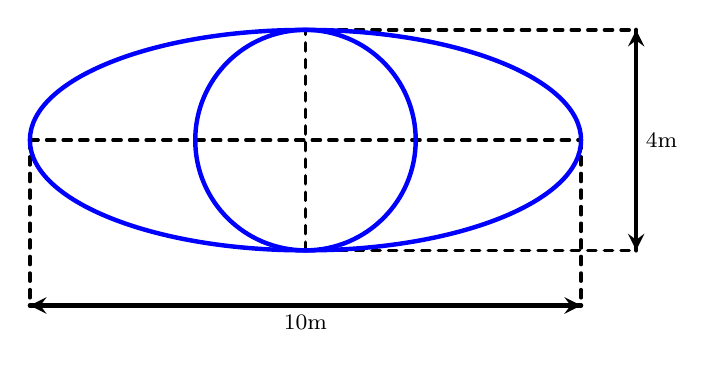
\begin{tikzpicture}[scale=0.7, font=\footnotesize, line join=round, line cap=round, >=stealth]
\draw[ultra thick, ->](6,-2)--(6,2);
\draw[ultra thick, ->](6,2)--(6,-2);
\draw[ultra thick, ->](-5,-3)--(5,-3);
\draw[ultra thick, ->](5,-3)--(-5,-3);
\draw[very thick, dashed](-5,0)--(5,0) (0,-2)--(0,2) (0,2)--(6,2) (0,-2)--(6,-2) (-5,0)--(-5,-3) (5,0)--(5,-3);
\draw(6,0)node[right]{$4$m} (0,-3)node[below]{$10$m};
\draw[ultra thick, blue](2,0)arc[x radius=2, y radius=2, start angle=0, end angle=360];
\draw[ultra thick, blue](5,0)arc[x radius=5, y radius=2, start angle=0, end angle=360];
\end{tikzpicture}
}
\loigiai
{
\begin{center}
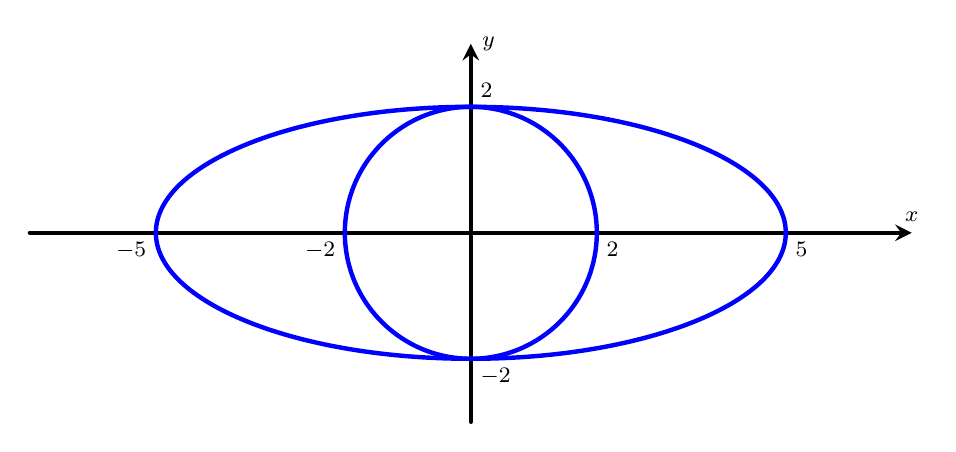
\begin{tikzpicture}[scale=0.8, font=\footnotesize, line join=round, line cap=round, >=stealth]
\draw(5,0)node[below right]{$5$} (-5,0)node[below left]{$-5$} (-2,0)node[below left]{$-2$} (2,0)node[below right]{$2$} (0,2)node[above right]{$2$} (0,-2)node[below right]{$-2$};
\draw[ultra thick, ->](-7,0)--(7,0)node[above]{$x$};
\draw[ultra thick, ->](0,-3)--(0,3)node[right]{$y$};
\draw[ultra thick, blue](2,0)arc[x radius=2, y radius=2, start angle=0, end angle=360];
\draw[ultra thick, blue](5,0)arc[x radius=5, y radius=2, start angle=0, end angle=360];
\end{tikzpicture}
\end{center}
Chọn hệ trục tọa độ $Oxy$ với gốc $O$ là tâm elip và tâm đường tròn. \\
Khi đó $(E)$ là elip chính tắc với $\heva{&a=5\\&b=2.}$ \\
Khi đó diện tích của $(E)$ là $S_{(E)}=\pi ab=10\pi$. \\
Diện tích vùng trồng hoa là $S_{(C)}=\pi R^2=\pi\cdot2^2=4\pi$. \\
Suy ra chi phí trồng hoa là $T_1=4\pi\cdot100\,000=400\,000\pi$. \\
Diện tích vùng trồng cỏ là $S=S_{(E)}-S_{(C)}=10\pi-4\pi=6\pi$. \\
Suy ra chi phí trồng cỏ là $T_2=6\pi\cdot60\,000=360\,000\pi$. \\
Vậy tổng chi phí mà ban tổ chức cần dùng là
\[T=T_1+T_2=400\,000\pi+360\,000\pi=760\,000\pi\approx2\,388\,000\,\text{đồng}\]. \\
}
\end{bt}

\begin{bt}%[2D4V1-6]
% nguon: Archive/SP-4Phan-Dot3/Data/CTST_2-OTGK2-De05.tex #4508

Cây cà chua khi trồng có chiều cao $5$ cm. Tốc độ tăng trưởng của cà chua sau khi trồng được cho bởi hàm số $v(t)=-0{,}1t^3+t^2$, trong đó $t$ tính theo tuần, $v(t)$ tính bằng centimét/tuần. Gọi $h(t)$ (tính bằng centimét) là độ cao của cây cà chua ở tuần thứ $t$. Tính chiều cao của cây cà chua tại thời điểm cây cà chua phát triển nhanh nhất.
\loigiai
{
Ta có $h(t)$ là một nguyên hàm của hàm số $v(t)$. \\
Ta có $h(t)=\displaystyle\int v(t)\mathrm{\,d}t=\displaystyle\int \left(-0{,}1t^3+t^2\right)\mathrm{\,d}t=-\dfrac{0{,}1t^4}{4}+\dfrac{t^3}{3}+C$. \\
Vì cây cà chua khi trồng cao $5$ cm nên $h(0)=5 \Leftrightarrow C=5$.\\
Suy ra $h(t)=-\dfrac{0{,}1t^4}{4}+\dfrac{t^3}{3}+5$. \\
Ta xác định thời điểm mà $v(t)$ đạt giá trị lớn nhất. \\
Ta có $v'(t)=-0{,}3t^2+2t$. \\
Xét $v'(t)=0 \Leftrightarrow \hoac{ & t=0 \\ & t=\dfrac{20}{3}.}$ \\
Bảng biến thiên của $v(t)$
\begin{center}

\begin{tikzpicture}
\tkzTabInit[nocadre=true, lgt=1.2, espcl=2.5, deltacl=0.6]{$t$/0.7, $v'(t)$/0.7, $v(t)$/2}{$0$, $\tfrac{20}{3}$, $+\infty$}
\tkzTabLine{,+,0,-,}
\tkzTabVar{-/, +/$v\left(\tfrac{20}{3}\right)$,-/}
\end{tikzpicture}
\end{center}
Thời điểm cây phát triển nhanh nhất, tức là $v(t)$ đạt giá trị lớn nhất thì $t=\dfrac{20}{3}$.\\
Vào thời điểm $t=\dfrac{20}{3}$ tuần, chiều cao của cây cà chua là $h\left(\dfrac{20}{3}\right)=\dfrac{4\,405}{81}\approx54{,}4$ (cm).
}
\end{bt}

\begin{bt}%[2D4H1-6]
% nguon: Archive/SP-4Phan-Dot3/Data/CTST_2-OTGK2-De01.tex #4516
%[Dự án đè thi 4 phần đợt 3]%[Đoàn Văn Mùi]
	\immini
	{Một con lắc lò xo dao động điều hòa theo phương ngang trên mặt phẳng không ma sát như hình bên, có vận tốc tức thời cho bởi $v(t)=4\cos{t}$, trong đó $t$ tính bằng giây và $v(t)$ tính bằng centimét/giây. Tại thời điểm $t=0$, con lắc ở vị trí cân bằng.\\
		Lập phương trình chuyển động của con lắc đó.}
	{\begin{tikzpicture}[scale=1, font=\footnotesize, line join=round, line cap=round, >=stealth]
			\def\xt{-1.5}
			\def\xp{3.2}
			\def\yd{0}
			\def\yt{2.5}
			\def\d{0.4}
			\pgfmathsetmacro{\h}{0.25*\d*(sqrt(3))}	
			\draw[line width=1mm, gray] (\xt,0.25)--++(0.3,0)--++(60:0.2);
			\foreach \i in {2,3,...,7}{\draw[line width=1mm, gray] (0.4*\i+\xt-0.5*\d,0.25-\h)--++(60:\d);}
			\draw[line width=1mm, gray] (0.4*8+\xt-0.5*\d,0.25-\h)--++(60:0.5*\d) --++(0:0.25);
			\foreach \i in {1,2,...,7}{\draw[line width=1mm, gray!60!white] (0.4*\i+\xt,0.25+\h)--++(-60:\d);}
			\fill[cyan] (8.5*\d+\xt-0.05,-0.5*\h) rectangle++(1.5*\d,4*\h);
			\fill[pattern=north west lines, draw=black] (\xt-0.2,\yd-0.5*\h) rectangle (\xt,\yt);
			\draw[->, thick] (\xt-0.2,\yd-0.5*\h)--(\xp,\yd-0.5*\h) node[below]{$x$};
			\draw (4.25*\d+\xt,{-0.05-0.5*\h})node[below]{$O$}--++(90:0.1)
			(9.25*\d+\xt-0.05,{-0.05-0.5*\h})node[below]{$x(t)$}--++(90:0.1);
			\draw[<-] (4.25*\d+\xt,{0.1+2*\h})--++(90:1)node[above]{\textrm{vị trí cân bằng}};	
	\end{tikzpicture}}
	\loigiai
	{Giả sử con lắc chuyển động theo phương trình $x=x(t)$, suy ra $v(t)=x'(t)$. Do đó $x(t)$ là một nguyên hàm của $v(t)$.\\
		Ta có $\displaystyle\int{v(t)}\,{\mathrm{d}t} = \displaystyle\int{4\cos{t}}\,{\mathrm{d}t} = 4\displaystyle\int{\cos{t}}\,{\mathrm{d}t} = 4\sin{t}+C$.\\
		Suy ra $x(t)=4\sin{t}+C$.\\
		Tại thời điểm $t=0$, con lắc ở vị trí cân bằng nên $x(t)=0$, suy ra $4\sin{0}+C=0 \Leftrightarrow C=0$.\\
		Vậy phương trình dao động của con lắc là $x(t)=4\sin{t}$.}
\end{bt}

\begin{bt}%[2D4V2-2]
% nguon: Archive/SP-4Phan-Dot3/Data/CTST_2-OTGK2-De01.tex #4517
%[Dự án đè thi 4 phần đợt 3]%[Đoàn Văn Mùi]
	Cho $F(x)$ là nguyên hàm của hàm số $f(x)$. Biết $F(-1)=1$ và $F(2)=4$. Tính $\displaystyle\int\limits_{-1}^2\left[ f(x)+2 x\right]  \mathrm{\,d}x$.
	\loigiai{
			 Ta có $I=\displaystyle\int\limits_{-1}^2\left[ f(x)+2 x\right]  \mathrm{d} x=\left[F(x)+x^2\right]\bigg|_{-1} ^2=F(2)+4-F(-1)-1=6$.
	}
\end{bt}

\begin{bt}%[2D4H3-1]
% nguon: Archive/SP-4Phan-Dot3/Data/CTST_2-OTGK2-De01.tex #4518
%[Dự án đè thi 4 phần đợt 3]%[Đoàn Văn Mùi]
	Cho hàm số $f(x)=x^2-4x$. Tính diện tích hình phẳng giới hạn bởi đồ thị hàm số $y=f(x)$ và $Ox$.
	\loigiai{
			Ta có $x^2-4x=0 \Leftrightarrow \hoac{&x=0\\&x=4.}$\\
			Bảng xét dấu
			\begin{center}
				
\begin{tikzpicture}
					\tkzTabInit[nocadre=false,lgt=1.5,espcl=2.5,deltacl=0.6]
					{$x$/0.7,$f(x)$/0.7}
					{$-\infty$,$0$,$4$,$+\infty$}
					\tkzTabLine{,+,0,-,0,+,}   
				\end{tikzpicture}
			\end{center}
			Suy ra $x^2-4x\le 0, \, \forall x \in [0;4]$.\\
			$S = \displaystyle \int \limits_{0}^{4}{\left| x^2-4x \right|}\mathrm{\,d}x =-\int \limits_{0}^{4}{\left( x^2-4x \right)}\mathrm{\,d}x = -\left(\dfrac{x^3}{3} - 2x^2\right)\bigg|_0^4 = \dfrac{32}{3}$.
	}
\end{bt}

\begin{bt}%[2D4H1-6]
% nguon: Archive/SP-4Phan-Dot3/Data/CTST_2-OTGK2-De02.tex #4526

		Một vật chuyển động có gia tốc là $a\left(t\right)=\dfrac{3}{t+1}$ (m/s$^2$). Biết rằng vận tốc ban đầu của vật là $6$ m/s. Vận tốc của vật đó sau $5$ giây là bao nhiêu m/s$^2$?
			\loigiai{
			Vận tốc của vật là $v(t)=\displaystyle \int a\left(t\right)\mathrm{\,d}t =\int \dfrac{3}{t+1}\mathrm{\,d}t=3\ln |t+1|+C$.\\
			Vì vận tốc tốc ban đầu của vật là $6$ m/s nên $v(0)=6 \Leftrightarrow 3\ln 1+C=6  \Leftrightarrow C=6$.\\
			Suy ra $v(t)=3\ln |t+1| +6$.\\
			Vận tốc của vật đó sau $10$ giây là $v(10)=3\ln|10+1|+6\approx 13{,}2$ (m/s).
		}
\end{bt}

\begin{bt}%[2D4N2-2]
% nguon: Archive/SP-4Phan-Dot3/Data/CTST_2-OTGK2-De02.tex #4527

	Tính tích phân $I=\displaystyle\int\limits _1^{\mathrm{e}} \dfrac{3}{t}\mathrm{\,d}t$.
	\loigiai{
		\begin{eqnarray*}
		I=\displaystyle\int\limits _1^{\mathrm{e}} \dfrac{3}{t}\mathrm{\,d}t
		&=&\big(3\ln|t|\big)\bigg|_1^{\mathrm{e}}\\
		&=&3\left(\ln\mathrm{e}-\ln 1\right) = 3(1-0)=3.	 
		\end{eqnarray*}
	
	}
\end{bt}

\begin{bt}%[2D4V1-6]
% nguon: Archive/SP-4Phan-Dot3/Data/CTST_2-OTGK2-De02.tex #4528

Người ta trồng hoa vào phần đất được tô màu đen được giới hạn bởi cạnh $AB$, $CD$  đường trung bình  $MN$ của mảnh đất hình chữ nhật  $ABCD$ và một đường cong hình sin (như hình vẽ). Biết $AB=2\pi$ (m), $AD=2$ (m). Tính diện tích phần đát còn lại.
	\begin{center}
	\begin{tikzpicture}[scale=1,>=stealth, font=\footnotesize, line join=round, line cap=round]
		\path 
		(-pi,1) coordinate (A)
		(pi,1) coordinate (B)
		(pi,-1) coordinate (C)
		(-pi,-1) coordinate (D)
		(-pi,0) coordinate (M)
		(pi,0) coordinate (N)
		;
		\draw (A)--(B)--(C)--(D)--cycle (M)--(N);
		\draw[smooth,samples=400,domain=-pi:pi] plot(\x,{sin(\x r)});
		\fill[pattern= north east lines] plot[domain=-pi:pi ](\x,{sin(\x r)});
		\foreach \x/\g in {A/150,B/30,C/-30,D/-150,M/180,N/0}
		\fill[black] 	(\x) circle (1pt)
		($(\g:3mm)+(\x)$) node {$\x$};
	\end{tikzpicture}
\end{center}
	\loigiai{
		\begin{center}
		\begin{tikzpicture}[scale=1,>=stealth, font=\footnotesize, line join=round, line cap=round]
			\path 
			(-pi,1) coordinate (A)
			(pi,1) coordinate (B)
			(pi,-1) coordinate (C)
			(-pi,-1) coordinate (D)
			(-pi,0) coordinate (M)
			(pi,0) coordinate (N)
			;
			\draw[->] (-4,0)--(4,0) node[below right]{$x$};
			\draw[->] (0,-1.5)--(0,1.5) node[left]{$y$};
			\node[below right] at (0,0) {$O$};
			\draw (A)--(B)--(C)--(D)--cycle (M)--(N);
			\draw[smooth,samples=400,domain=-pi:pi] plot(\x,{sin(\x r)});
			\fill[pattern= north east lines] plot[domain=-pi:pi ](\x,{sin(\x r)});
			\foreach \x/\g in {A/150,B/30,C/-30,D/-150,M/135,N/45}
			\fill[black] 	(\x) circle (1pt)
			($(\g:3mm)+(\x)$) node {$\x$};
		\end{tikzpicture}
		\end{center}
		Chọn hệ trục tọa độ $Oxy$ như hình vẽ. Khi đó\\
		Diện tích hình chữ nhật $ABCD$ bằng $S_1=AB\cdot AD=4\pi$.\\
		Diện tích phần đất trồng hoa bằng
		$$S_2=2\displaystyle\int\limits_{0}^{\pi} \sin x \mathrm{\,d}x 
		= -2\cos x \Big|_{0}^{\pi}
		= -2\left(\cos 0 - \cos\pi\right)=4.$$
		Suy ra phần đất còn lại bằng $S=S_1-S_2=4\pi -4 =4(\pi -1)$ m$^2$.
	}
\end{bt}

\begin{bt}%[2D4V1-3]
% nguon: Archive/SP-4Phan-Dot3/Data/CTST_2-OTGK2-De03.tex #4535

	Gọi $F(x)$ là nguyên hàm của hàm số $f(x)=\sin^2x$ thỏa mãn $F(0)=0$. Giải phương trình $2F(x)-x=0$. 
	\loigiai{$F(x)=\displaystyle\int\limits f(x)\mathrm{\,d}x=\displaystyle\int\limits \sin^2x\mathrm{\,d}x=\displaystyle\int\limits \left( \dfrac{1}{2}-\dfrac{1}{2}\cos2x\right) \mathrm{\,d}x=\dfrac{x}{2}-\dfrac{\sin2x}{4}+C$.\\
	Vì $F(0)=0$ nên $C=0$.\\
	Suy ra $F(x)=\dfrac{x}{2}-\dfrac{\sin2x}{4}$.\\
	Khi đó, $$2F(x)-x=0\Leftrightarrow \sin 2x=0\Leftrightarrow x=\dfrac{k\pi}{2}, k\in \mathbb{Z}.$$
	}
\end{bt}

\begin{bt}%[2D4V3-4]
% nguon: Archive/SP-4Phan-Dot3/Data/CTST_2-OTGK2-De03.tex #4536

\immini{Khi cắt vật thể bởi mặt phẳng vuông góc với trục $Ox$ tại điểm có hoành độ là $x$ ($0 \leq x \leq 3$), ta được mặt cắt là một hình vuông có cạnh là $\sqrt{9 - x^2}$ (xem hình dưới). Tính thể tích của vật thể đã
	cho.}{
		\begin{tikzpicture}[>=stealth,line join=round,line cap=round,font=\footnotesize,scale=1]
			%\clip (-2,-0.7) rectangle (4.5,3);	
			\path
			(0,0) coordinate (O)
			(3.37,0) coordinate (A)
			(5.2,1.5) coordinate (B)
			($(O)-(A)+(B)$) coordinate (C)
			($(A)+(0,2.24)$) coordinate (A')
			($(B)+(0,2.24)$) coordinate (B')
			($(O)+(0,1.6)$) coordinate (O')
			($(C)+(0,1.6)$) coordinate (C')
			($(O)!0.75!(A)$) coordinate (M)
			($(C)!0.75!(B)$) coordinate (N)
			($(O')!0.75!(A')$) coordinate (Q)
			($(C')!0.75!(B')$) coordinate (P)
			;
			\draw[->,line width = 1pt] (O) node[below left]{$O$}--(6.5,0) node[below]{$x$};
			\fill (A) node[below]{$3$};
			\fill (M) node[below]{$x$};
			\fill[cyan!10] (M)--(N)--(P)--(Q)--cycle;
			\draw (A)--(B)--(B')--(C')--(O')--(A')--(A) (A')--(B') (O)--(O');
			\draw[dashed] (O)--(C)--(B) (C)--(C');
			\fill (2.6,1) node[left,scale=0.8]{$\sqrt{9 - x^2}$};
			\fill (3.37,2) node[right]{$S(x)$};
			\draw[cyan,thick] (M)--(Q)--(P);
			\draw[dashed,cyan,thick] (M)--(N)--(P);
		\end{tikzpicture}}
	\loigiai{
		Ta có mặt cắt của vật thể là một hình vuông có cạnh là $\sqrt{9 - x^2}$ nên diện tích mặt cắt là
		$$ S(x) = \left(\sqrt{9 - x^2}\right)^2 = 9 - x^2, \textrm{ do $9 - x^2 \geq 0$, $\forall x \in [0;3]$.} $$
		Thể tích của vật thể đã cho là
		$$ V = \displaystyle\int\limits_{0}^{3} S(x)\mathrm{\,d}x = \displaystyle\int\limits_{0}^{3} \left(9 - x^2\right)\mathrm{\,d}x = \left(9x - \dfrac{x^3}{3}\right)\Bigg|_{0}^{3} = 18~(\text{đvdt}). $$
	}
\end{bt}

\begin{bt}%[2D4H2-3]
% nguon: Archive/SP-4Phan-Dot3/Data/CTST_2-OTGK2-De03.tex #4538

	Tính tích phân sau
	 $\displaystyle\int\limits_1^2 \dfrac{x-1}{x^2} \mathrm{\,d} x$.
		\loigiai{
	Ta có $\displaystyle\int\limits_1^2 \dfrac{x-1}{x^2} \mathrm{\,d} x=\displaystyle\int\limits_1^2\left(\dfrac{1}{x}-\dfrac{1}{x^2}\right) \mathrm{\,d} x=\displaystyle\int\limits_1^2 \dfrac{1}{x}\mathrm{\,d} x-\displaystyle\int\limits_1^2 \dfrac{1}{x^2} \mathrm{\,d} x= \ln x\bigg|_1^2+\left.\dfrac{1}{x}\right|_1^2=\ln 2-\dfrac{1}{2}$.}
\end{bt}

\begin{bt}%[2D4C3-3]
% nguon: Archive/SP-4Phan-Dot3/Data/CTST_2-OTHK2-De04.tex #4556

	\immini[thm]{
		Một vật trang trí có dạng một khối tròn xoay được tạo thành khi xoay miền $(R)$ (phần gạch chéo trong hình vẽ bên) quanh trục $AB$. Miền $(R)$ được giới hạn bởi các cạnh $AB$, $AD$ của hình vuông $ABCD$ và các cung phần tư của các đường tròn bán kính bằng $1$ cm với tâm lần lượt là trung điểm của các cạnh $BC$, $AD$. Tính thể tích của vật trang trí đó (đơn vị cm$^3$).
	}{
		\begin{tikzpicture}
			\coordinate (A) at (0,0);
			\coordinate (B) at (0,-4);
			\coordinate (C) at (4,-4);
			\coordinate (D) at (4,0);
			\draw (A)--(B)--(C)--(D)--(A);
			\draw[pattern=north east lines] (B) arc (180:90:2) arc (-90:0:2)--(A)--(B);
			\path node at (A) [above left]{$A$}
			node at (B) [below left] {$B$}
			node at (C) [below right] {$C$}
			node at (D) [above right] {$D$};
		\end{tikzpicture}
	}
	\loigiai{
		\begin{center}
			\begin{tikzpicture}
				\draw [->] (0,-4) --(5,-4);
				\draw [->] (0,-4) --(0,1);
				\coordinate (D) at (0,0);
				\coordinate (A) at (0,-4);
				\coordinate (B) at (4,-4);
				\coordinate (C) at (4,0);
				\coordinate (I) at (4,-2);
				\coordinate (J) at (0,-2);
				\coordinate (K) at (2,-2);
				\draw (A)--(B)--(C)--(D)--(A);
				\draw[pattern=north west lines,opacity=0.4] (D) arc (90:0:2) arc (180:270:2)--(B)--(A)--(D);
				\foreach \x in {A,B,C,D,I,J,K}{
					\fill (\x) circle (1pt);
				}
				
				\draw[line width=1.5pt, red] (D) arc (90:0:2);
				\draw[dashed, opacity=0.4,red] (D) arc (90:450:2); 
				\draw[line width=1.5pt, blue] (K) arc (180:270:2);
				\draw[dashed, opacity=0.4,blue] (K) arc (180:540:2);
				
				\path node at (D) [above left]{$D$}
				node at (A) [below left] {$A\equiv O$}
				node at (B) [below right] {$B$}
				node at (C) [above right] {$C$}
				node at (I) [left] {$I$}
				node at (J) [left] {$J$}
				node at (5,-4) [below] {$x$}
				node at (0,1) [left] {$y$}
				node at (K) [right] {$K$}
				node at (2.6,-0.3) {$y=1+\sqrt{1-x^2}$}
				node at (4.2,-3) {$y=1-\sqrt{1-(x-2)^2}$};
			\end{tikzpicture}
		\end{center}
		Ta xoay hình lại và đưa vào hệ trục tọa độ như trên hình vẽ. Khi đó phần gạch chéo trên hình sẽ quay quanh trục $Ox$.\\
		Đường tròn tâm $J$
		\allowdisplaybreaks
		\begin{eqnarray*}
			x^2+(y-1)^2=1&\Rightarrow& (y-1)^2=1-x^2\\
			& \Leftrightarrow& |y-1|=\sqrt{1-x^2}\\
			& \Leftrightarrow &\heva{& y-1 =\sqrt{1-x^2}, \mbox{ khi } y\ge 1 \\& -(y-1) =\sqrt{1-x^2}, \mbox{ khi } y< 1} \\
			&\Leftrightarrow& \heva{& y =1+\sqrt{1-x^2}, \mbox{ khi } y\ge 1 \\& y=1-\sqrt{1-x^2} , \mbox{ khi } y< 1.}
		\end{eqnarray*}	
		Suy ra đồ thị đường cong từ $D$ đến $K$ là $y=1+\sqrt{1-x^2}$ với $x\in [0;1]$.\\	
		Đường tròn tâm $I$
		\begin{eqnarray*}
			(x-2)^2+(y-1)^2=17&\Rightarrow& (y-1)^2=1-(x-2)^2 \\
			&\Leftrightarrow& |y-1|=\sqrt{1-(x-2)^2}\\
			&\Leftrightarrow& \heva{& y-1 =\sqrt{1-(x-2)^2}, \mbox{ khi } y\ge 1 \\& -(y-1) =\sqrt{1-(x-2)^2}, \mbox{ khi } y< 1}\\
			&\Leftrightarrow& \heva{& y =1+\sqrt{1-(x-2)^2}, \mbox{ khi } y\ge 1 \\& y=1-\sqrt{1-(x-2)^2} , \mbox{ khi } y< 1}
		\end{eqnarray*}
		Suy ra đồ thị đường cong từ $K$ đến $B$ là $y=1-\sqrt{1-(x-2)^2}$ với $x\in [1;2]$.\\	
		Đường cong đi từ $D$ đến $B$ trên hình gồm hai phần$\colon$ phần thứ nhất là một phần tư đường tròn đi từ $D$ đến $K$ của đường tròn tâm $J$ và phần thứ hai là một phần tư đường tròn đi từ $K$ đến $B$ của đường tròn tâm $I$.\\
		Thể tích của vật trang trí là
		$$V= \pi\displaystyle\int\limits_0^1 \left(1+\sqrt{1-x^2}\right)^2\mathrm{\,d}x +  \pi\displaystyle\int\limits_1^2 \left(1-\sqrt{1-(x-2)^2}\right)^2\mathrm{\,d}x \approx 10{,}5 \mbox{ cm}^3.$$
	}
\end{bt}

\begin{bt}%[2D4V3-2]
% nguon: Archive/SP-4Phan-Dot3/Data/CTST_2-OTHK2-De06.tex #4561

	Một cái cổng có kích thước như hình a. Vòm cổng có hình dạng một parabol có đỉnh $I(0 ; 2)$ và đi qua điểm $B\left(\dfrac{5}{2} ; \dfrac{3}{2}\right)$ như hình b. Tính diện tích hai cánh cửa cổng (\textit{kết quả làm tròn đến hàng phần trăm}).
	\begin{center}
		\begin{tikzpicture}[scale=1, font=\footnotesize, line join=round, line cap=round,>=stealth]
			\fill[color=brown, draw=none] (-5/2,0)--(-5/2,3/2)--plot[domain=-5/2:5/2](\x,{-2/25*(\x)^2+2})--(5/2,3/2)--(5/2,0)--cycle;
			\draw[fill=orange,draw=none] (-3.5,-0.05) rectangle (-2.55,1.7);
			\draw[fill=orange,draw=none] (2.55,-0.05) rectangle (3.5,1.7);
			\draw[fill=gray!50,draw=none] (-3.6,1.7) rectangle (-2.5,1.85);
			\draw[fill=gray!50,draw=none] (2.5,1.7) rectangle (3.6,1.85);
			\draw[fill=black,draw=none] (-3.3,1.85) rectangle (-2.8,1.9);
			\draw[fill=black,draw=none] (2.8,1.85) rectangle (3.3,1.9);
			\draw[fill=black,draw=none] (-3.1,1.9) rectangle (-3,2);
			\draw[fill=black,draw=none] (3,1.9) rectangle (3.1,2);
			\draw[fill=orange!70,draw=none] (-3.05,2.2) circle (0.2);
			\draw[fill=orange!70,draw=none] (3.05,2.2) circle (0.2);
			\draw[fill=black,draw=none] (-2.55,0.4) rectangle (-2.5,0.65);
			\draw[fill=black,draw=none] (-2.55,1.05) rectangle (-2.5,1.3);
			\draw[fill=black,draw=none] (2.5,0.4) rectangle (2.55,0.65);
			\draw[fill=black,draw=none] (2.5,1.05) rectangle (2.55,1.3);
			\draw[color=white] (0,0)--(0,2);
			\draw (0,2)--(5,2) (5/2,3/2)--(4.4,3/2) (0,0)--(5,0) (-3.5,-0.1)--(-3.5,-0.5) (3.5,-0.1)--(3.5,-0.5);
			\draw[<->] (-3.5,-0.3)--(3.5,-0.3);
			\draw[<->] (4.2,0)--(4.2,3/2);
			\draw[<->] (4.8,0)--(4.8,2);
			\node at (0,-0.5){$5~\mathrm{m}$};
			\node[rotate=90] at (4.6,1){$2~\mathrm{m}$};
			\node[rotate=90] at (3.9,0.75){$\tfrac{3}{2}~\mathrm{m}$};
			\node[below] at (current bounding box.south){$a)$};
		\end{tikzpicture}
		\begin{tikzpicture}[scale=1, font=\footnotesize, line join=round, line cap=round,>=stealth]
			\draw[->] (-3.5,0) --(3.5,0) node[below]{$x$};
			\draw[->] (0,-0.75) --(0,3) node[left]{$y$};
			\draw (0,0) node[below left=-3pt]{$O$};
			\draw[smooth,samples=200,domain=-5/2:5/2] plot(\x,{-2/25*(\x)^2+2});
			\draw (-5/2,3/2)--(-5/2,0)--(5/2,0)--(5/2,3/2);
			\draw[dashed] (-5/2,3/2)--(5/2,3/2);
			\draw[fill=black]
			(-5/2,0) node[below]{$-\tfrac{5}{2}$} circle (1pt)
			(5/2,0) node[below]{$\tfrac{5}{2}$} circle (1pt)
			(0,3/2) node[below left]{$\tfrac{3}{2}$} circle (1pt)
			(-5/2,3/2) node[left]{$A$} circle (1pt)
			(5/2,3/2) node[right]{$B$} circle (1pt)
			(0,2) node[above right]{$2$} circle (1pt)
			(0,2) node[above left]{$I$}
			(-5/2,0) node[above left]{$D$}
			(5/2,0) node[above right]{$C$}
			;
			\node[below] at (current bounding box.south){$b)$};
		\end{tikzpicture}
	\end{center}
	\loigiai{
		Vòm cổng có hình dạng một parabol $(P)$ có đỉnh $I(0 ; 2)$ nên có phương trình dạng $y=ax^2+2$. Mặt khác $(P)$ đi qua điểm $B\left(\dfrac{5}{2} ; \dfrac{3}{2}\right)$ nên ta có
		$$\dfrac{3}{2}=a\cdot \left(\dfrac{5}{2}\right)^2+2\Leftrightarrow \dfrac{25}{4}a=-\dfrac{1}{2}\Leftrightarrow a=-\dfrac{2}{25}.$$
		Do đó $(P)\colon y=-\dfrac{2}{25}x^2+2$.\\
		Gọi $S~\left(\mathrm{m}^2\right)$ là tổng diện tích hai cánh cửa cổng.\\
		Khi đó $S$ bằng diện tích hình phẳng giới hạn bởi parabol $(P)$, trục hoành và hai đường thẳng $x=-\dfrac{5}{2}$, $x=\dfrac{5}{2}$. Vậy
	 	\[S=\int\limits_{-\tfrac{5}{2}}^{\tfrac{5}{2}}\left(-\dfrac{2}{25}x^2+2\right)\,\mathrm{d}x=\left.\left(-\dfrac{2}{75}x^3+2x\right)\right|_{-\tfrac{5}{2}}^{\tfrac{5}{2}}=\dfrac{55}{6}\approx 9{,}17~\left(\mathrm{m}^2\right).\]
	}
\end{bt}

\begin{bt}%[2D4V3-4]
% nguon: Archive/SP-4Phan-Dot3/Data/CTST_2-OTHK2-De03.tex #4571

	Khi cắt một vật thể hình chiếc nêm bởi mặt phẳng vuông góc với trục $Ox$ tại điểm có hoành độ $x$ (với $-2\le x\le 2$), mặt cắt là tam giác vuông có một góc bằng $45^{\circ}$ và độ dài một cạnh góc vuông là $\sqrt{4-x^2}$ (dm). Được mô tả như hình vẽ bên dưới.
	\begin{center}
		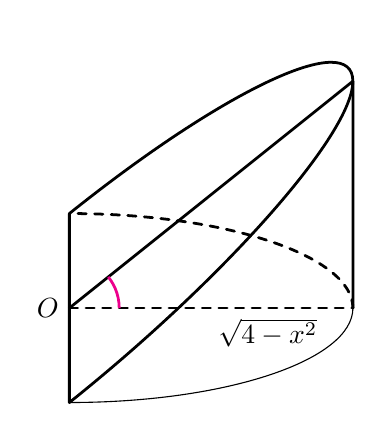
\begin{tikzpicture}[line join=round, line cap=round,scale=1.2, >=stealth]
			\tikzset{label style/.style={font=\footnotesize}}
			\def\a{3}
			\def\b{1}
			\def\h{5}
			\coordinate (O) at (0,0);
			\coordinate (A) at (\a,0);
			\coordinate (B) at (0,\b);
			\draw[dashed,line width=1pt] (A) arc(0:90:{\a} and {\b});
			\draw (A) arc(0:-90:{\a} and {\b});
			\draw[line width=1pt,yslant=.8] (B) arc(90:0:{\a} and {\b}) coordinate (C);
			\draw[line width=1pt,yslant=.8] (0,-\b) arc (-90:0:{\a} and {\b});
			\draw [line width=1pt] (B)--(0,-\b) (O)--(C)--(A) ;
			\draw[dashed, line width=1pt] (O)node [left]{$O$}--(A)node [below,pos=.7]{$\sqrt{4-x^2}$};
			\clip (C)--(O)--(A);
			\draw[magenta,line width=1pt] (0,0) circle(15pt);
		\end{tikzpicture}
	\end{center}
	Biết thể tích của vật thể có dạng $V=\dfrac{a}{b}$ (dm$^3$) (với $a$, $b$ là các số nguyên dương và $\dfrac{a}{b}$ tối giản. Tính giá trị của biểu thức $T=a^b$.
	\loigiai{
		Thiết diện là một tam giác vuông cân có diện tích là $S(x)=\dfrac{1}{2}{{\left(\sqrt{4-x^2} \right)}^2}=\dfrac{1}{2}\left(4-x^2 \right)$.\\
		Thể tích cần tìm là $V=\displaystyle\int\limits_{-2}^2{S(x)\mathrm{\,d}x}=\displaystyle\int\limits_{-2}^2{\dfrac{1}{2}\left(4-x^2 \right)x}=\dfrac{16}{3}\,\,\left(\mathrm{dm}^3 \right)$.\\
		Theo đề ta có $V=\dfrac{a}{b}$\, (dm$^3 $) $\Rightarrow a=16$; $b=3$.\\
		Suy ra $T=a^b={16}^3=4\,096$.
	}
\end{bt}

\begin{bt}%[2D4V3-3]
% nguon: Archive/SP-4Phan-Dot3/Data/CTST_2-OTHK2-De02.tex #4581

    \immini
    {Một vật trang trí có dạng một khối tròn xoay được tạo thành khi quay miền $(R)$ (phần gạch chéo trong hình vẽ) quanh trục $MN$. Biết rằng $ABCD$ là hình chữ nhật với $AB=6$ cm, $AD=10$ cm. $M$, $N$ lần lượt là trung điểm của $AB$, $CD$, hai đường cong là đường elip có hình chữ nhật cơ sở là $ABCD$ và đường tròn tiếp xúc với hai cạnh $AD$ và $BC$ (tham khảo hình vẽ). Tính thể tích của vật trang trí đó (kết quả làm tròn đến hàng phần chục).}
    {\begin{tikzpicture}[scale=0.5]
            \def\r{5}
            \def\a{3}
            \draw[]
            (180:\r) arc (180:0:{\r} and {0.6*\r})
            (180:\r) arc (180:360:{\r} and {0.6*\r});
            \draw[pattern=north east lines]
            (0:\r) arc (0:360:{\r} and {0.6*\r});
            \draw[fill=white]
            (0:0) circle(0.6*\r);
            \path 	(180:5) coordinate (M)
            (0:5) coordinate (N)
            ($(M)+(90:\a)$) coordinate (A)
            ($(N)+(90:\a)$) coordinate (D)
            ($(M)+(-90:\a)$) coordinate (B)
            ($(N)+(-90:\a)$) coordinate (C);
            %\draw[dashed,thick] 	(B)--(D);
            \draw[thick] 			(B)--(A)--(D) (B)--(C)--(D);
            \foreach \x/\g in {A/90,B/180,C/-45,D/0,M/180,N/0}
            \fill[black] 	(\x) circle (1.5pt)
            ($(\g:4mm)+(\x)$) node {$\x$};
    \end{tikzpicture}}
    \loigiai{
    \immini
    {Chọn hệ trục tọa độ $Oxy$ với $O$ là trung điểm của $MN$, trục $Ox$ trùng với $MN$ như hình vẽ.\\
    Khi đó đường elip có hình chữ nhật cơ sở là $ABCD$ có phương trình là $\dfrac{x^2}{25}+\dfrac{y^2}{9}=1$ và đường tròn có phương trình $x^2+y^2=9$.\\
    Một nửa elip phía trên trục $Ox$ có phương trình $y=f(x)=\dfrac{3}{5}\sqrt{25-x^2}$. Do đó thể tích khối tròn xoay sinh bởi elip đó khi quay quanh trục $Ox$ bằng
    }
    {\begin{tikzpicture}[scale=0.5]
            \def\r{5}
            \def\a{3}
            \draw[]
            (180:\r) arc (180:0:{\r} and {0.6*\r})
            (180:\r) arc (180:360:{\r} and {0.6*\r});
            \draw[pattern=north east lines]
            (0:\r) arc (0:360:{\r} and {0.6*\r});
            \draw[fill=white]
            (0:0) circle(0.6*\r);
            \path 	(180:5) coordinate (M)
            (0:5) coordinate (N)
            ($(M)+(90:\a)$) coordinate (A)
            ($(N)+(90:\a)$) coordinate (D)
            ($(M)+(-90:\a)$) coordinate (B)
            ($(N)+(-90:\a)$) coordinate (C);
            %\draw[dashed,thick] 	(B)--(D);
            \draw[thick] 			(B)--(A)--(D) (B)--(C)--(D);
            \foreach \x/\g in {A/90,B/180,C/-45,D/0,M/150,N/40}
            \fill[black] 	(\x) circle (1.5pt)
            ($(\g:4mm)+(\x)$) node {$\x$};
            \draw[->] (-6,0)--(7,0)node[below]{$x$};
            \draw[->] (0,-3.5)--(0,4)node[right]{$y$};
            \draw (0,0)node[below right]{$O$};
    \end{tikzpicture}}
         $$V_1=\pi\displaystyle\int\limits_{-5}^{5}f^2(x)\mathrm{d}x=\pi\left(9x-\dfrac{3x^3}{25}\right)\bigg|_{-5}^5=60\pi.$$
        Phần hình tròn bên trong khi quay quanh trục $Ox$ tạo thành khối cầu có bán kính bằng $R=3$ nên có thể tích là $$V_2=\dfrac{4}{3}\pi R^3=36\pi.$$
        Do vậy thể tích của vật trang trí đó khi quay quanh trục $Ox$ bằng $$V_1-V2=24\pi\approx 75{,}4\,\textrm{cm}^3.$$
    }
\end{bt}

\begin{bt}%[2D4V3-2]
% nguon: Archive/SP-4Phan-Dot3/Data/CTST_2-OTHK2-De01.tex #4593

	\immini{
		Một cái cổng hình parabol như hình bên. Chiều cao $GH=4$ m, chiều rộng $AB=4$ m, $AC=BD=0{,}9$ m. Người ta làm hai cánh cổng khi đóng lại là hình chữ nhật $CDEF$ tô đậm với giá $1\,200\,000$ đồng/m$^2$, phần còn lại làm khung hoa sắt với giá $900\,000$ đồng/m$^2$. Hỏi chi phí để làm hai phần nói trên bằng bao nhiêu?
	}
	{
		\begin{tikzpicture}[scale=0.8,>=stealth, font=\footnotesize, line join=round, line cap=round]  
			\path
			(-2,0) coordinate (A)
			(2,0) coordinate (B)
			(-1.1,0) coordinate (C)
			(1.1,0) coordinate (D)
			(-1.1,2.79) coordinate (F)
			(1.1,2.79) coordinate (E)
			(0,0) coordinate (H)
			(0,4) coordinate (G)
			;
			\draw[fill,gray!50] (C)--(D)--(E)--(F)--cycle;
			\draw (A)--(B) (C)--(D)--(E)--(F)--cycle;
			\draw[dashed] (G)--(H);
			\draw [black, red, thick, domain=-2:2, samples=100] %
			plot (\x, {-(\x)^2+4});
			\foreach \i/\g in {A/-90,B/-90,C/-90,D/-90,E/30,F/150,H/-90,G/90}{\draw[fill=black](\i) circle (1.5pt) ($(\i)+(\g:4mm)$) node[scale=1]{$\i$};}
			\node[] at (0,-1.5) {\textit{Hình 4.31}};
		\end{tikzpicture}
	}
	\loigiai{
		\immini{
			Chọn hệ trục $Oxy$ với gốc tọa độ $H$ là trung điểm của $AB$.\\
			Khi đó $A(-2;0)$, $B(2;0)$ và $G(0;4)$.\\
			Gọi phương trình parabol có dạng $(P)\colon y=ax^2+c$.\\
			Do $(P)$ đi qua $A$ và $G$ nên ta có hệ $\heva{&4a+c=0\\&c=4}\Leftrightarrow \heva{&a=-1\\&c=4.}$\\
			Suy ra parabol $(P)\colon y=-x^2+4$.\\
			Diện tích hình phẳng giới hạn bởi parabol $(P)$ và trục hoành là
			$$S=\displaystyle \int\limits_{-2}^2\left(-x^2+4 \right) \mathrm{\,d}x=\dfrac{32}{3}.$$
		}
		{
			\begin{tikzpicture}[scale=0.8,thick,>=stealth, font=\footnotesize, line join=round, line cap=round]  
				\path
				(-2,0) coordinate (A)
				(2,0) coordinate (B)
				(-1.1,0) coordinate (C)
				(1.1,0) coordinate (D)
				(-1.1,2.79) coordinate (F)
				(1.1,2.79) coordinate (E)
				(0,0) coordinate (H)
				(0,4) coordinate (G)
				;
				\draw[fill,gray!50] (C)--(D)--(E)--(F)--cycle;
				\draw (A)--(B) (C)--(D)--(E)--(F)--cycle;
				\draw [black, red, thick, domain=-2:2, samples=100] %
				plot (\x, {-(\x)^2+4});
				%Vẽ hệ trục
				\draw[->] (-2.7,0)--(2.7,0) node[below]{$x$};
				\draw[->] (0,-1)--(0,5) node[left]{$y$};
				\draw[thin] (2,2pt)--(2,-2pt) + (60:4mm) node {\scriptsize $2$};
				\draw[thin] (-2,2pt)--(-2,-2pt) + (145:5mm) node {\scriptsize $-2$};
				\draw[thin] (2pt,4)--(-2pt,4) + (120:3mm) node {\scriptsize $4$};
				\foreach \i/\g in {A/-90,B/-90,C/-90,D/-90,E/30,F/150,H/-45,G/45}{\draw[fill=black](\i) circle (1.5pt) ($(\i)+(\g:4mm)$) node[scale=1]{$\i$};}
				
			\end{tikzpicture}
		}
		\noindent
		Ta có $AB=4$, $AC=BD=0{,}9 \Rightarrow CH=AH-AC=2-0{,}9=1{,}1$.\\
		Suy ra $C(-1{,}1;0)$, $D(1{,}1;0)$.\\
		$E(1{,}1;y_E) \in (P) \Leftrightarrow y_E=-(1{,}1)^2+4=2{,}79$.
		Suy ra $ED=2{,}79$.\\
		Diện tích hình chữ nhật $CDEF$ là $S_1=CD\cdot ED=2{,}2\cdot 2{,}79=6{,}138$.\\
		Diện tích khung hoa sắt là $S_2=S-S_1\approx 4{,}53 $.\\
		Chi phí để làm hai phần nói trên là $S_1\cdot 1\,200\,000+ S_2\cdot 900\,000\approx 11\,441\,400 $ đồng.
	}
\end{bt}
